\chapter{Foundations: Fields, Particles, and Locality}

\section{What is Quantum Field Theory?}

\[
\text{Q: What is QFT?}
\qquad
\text{A: QM + locality}
\]

\begin{center}
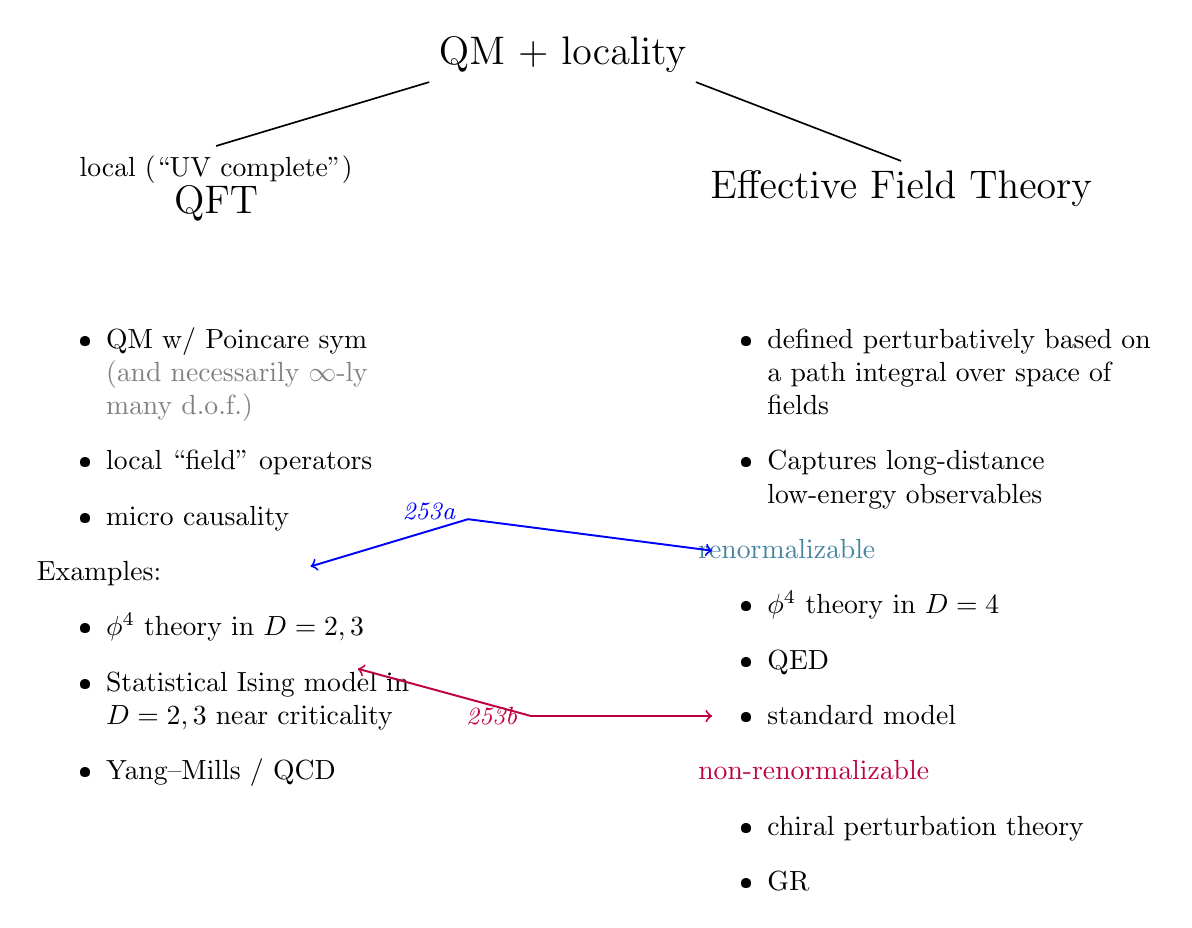
\begin{tikzpicture}[
  every node/.style={align=left},
  branch/.style={line width=0.6pt},
  note/.style={font=\small\itshape}
]
\node (root) at (0,0) {\Large QM + locality};
\node[align=center] (local) at (-4.4,-1.7) {local (``UV complete'')\\ \Large QFT};
\node[align=center] (eft) at (4.3,-1.7) {\Large Effective Field Theory};
\draw[branch] (root.south west) -- (local.north);
\draw[branch] (root.south east) -- (eft.north);

\node[text width=5.0cm,anchor=north west] at (-6.8,-2.9) {
\begin{itemize}
  \item QM w/ Poincare sym\\
  {\color{gray}(and necessarily $\infty$-ly many d.o.f.)}
  \item local ``field'' operators
  \item micro causality
\end{itemize}
Examples:
\begin{itemize}
  \item $\phi^4$ theory in $D=2,3$
  \item Statistical Ising model in $D=2,3$ near criticality
  \item Yang--Mills / QCD
\end{itemize}
};

\node[text width=5.8cm,anchor=north west] at (1.6,-2.9) {
\begin{itemize}
  \item defined perturbatively based on a path integral over space of fields
  \item Captures long-distance low-energy observables
\end{itemize}
\textcolor{cyan!60!black}{renormalizable}
\begin{itemize}
  \item $\phi^4$ theory in $D=4$
  \item QED
  \item standard model
\end{itemize}
\textcolor{purple}{non-renormalizable}
\begin{itemize}
  \item chiral perturbation theory
  \item GR
\end{itemize}
};

\node[note,blue] at (-1.7,-5.8) {253a};
\draw[->,blue,line width=0.7pt] (-1.2,-5.9) -- (-3.2,-6.5);
\draw[->,blue,line width=0.7pt] (-1.2,-5.9) -- (1.9,-6.3);
\node[note,purple] at (-0.9,-8.4) {253b};
\draw[->,purple,line width=0.7pt] (-0.4,-8.4) -- (-2.6,-7.8);
\draw[->,purple,line width=0.7pt] (-0.4,-8.4) -- (1.9,-8.4);
\end{tikzpicture}
\end{center}

\section{Plan of the Course}

\begin{enumerate}
\item Lagrangian formulation of QM
\begin{itemize}
  \item path integral, regularization
  \item perturbation theory, Feynman diagrams
  \item renormalization and counter terms
\end{itemize}

\item Relativistic particles and fields
\begin{itemize}
  \item $\phi^4$ theory
  \item Green functions
  \item asymptotic states
  \item S-matrix, LSZ reduction
\end{itemize}

\item Particles and fields with spin
\begin{itemize}
  \item classification of relativistic particles
  \item fermions and gauge bosons
  \item QED
  \item Applications: electron $g$-factor, Lamb shift.
\end{itemize}
\end{enumerate}

\section{Relativistic Particles}

Prelude: why do we need ``field theory'' to describe QM of particles with
relativistic symmetry?

\begin{itemize}
  \item Hilbert space $\mathcal H$
  \begin{itemize}
    \item vacuum $\ket{\Omega}$,
    \[
      H\ket{\Omega}=0.
    \]
    \item single particle $\ket{\vec p}$,
    \[
      p^\mu=(p^0,\vec p)
      \qquad
      \text{$D$-dimensional}
    \]
    \[
      H\ket{\vec p}=\sqrt{\vec p^{\,2}+m^2}\ket{\vec p}.
    \]
    \item multi-particle
    \[
      \ket{\vec p_1,\ldots,\vec p_n}
      \qquad
      \text{(non-interacting)}
    \]
    \[
      H=\sum_i \sqrt{\vec p_i^{\,2}+m^2}.
    \]
  \end{itemize}
\end{itemize}

Equivalently, we can introduce creation and annihilation operators:
\[
  \ket{\vec p}=a^\dagger_{\vec p}\ket{\Omega}.
\]

\[
  \ket{\vec p_1,\vec p_2}
  =
  a^\dagger_{\vec p_1}a^\dagger_{\vec p_2}\ket{\Omega},
  \qquad \text{etc.}
\]

\[
  [a,a]=[a^\dagger,a^\dagger]=0,
  \qquad
  [a_{\vec p},a^\dagger_{\vec p'}]
  =
  \delta^{(D-1)}(\vec p-\vec p'),
\]
so that
\[
  \braket{\vec p}{\vec p'}
  =
  \delta^{(D-1)}(\vec p-\vec p').
\]

We can then express the Hamiltonian as
\[
  H
  =
  \int \dd^{D-1}\vec p\,
  \sqrt{\vec p^{\,2}+m^2}\,
  a^\dagger_{\vec p}a_{\vec p}.
\]

This is a QM system of free relativistic particles.

What about interacting particles?
\[
  H=H_0+H_{\mathrm{int}},
\]
with possible terms such as
\[
  a^\dagger a^\dagger a,\qquad
  a a a^\dagger,\qquad \ldots
\]

It is not easy to find $H_{\mathrm{int}}$ that respects relativistic symmetry!

\section{Causality and Local Field Operators}

Issue: causality.

\begin{center}
\begin{tikzpicture}[scale=0.95,>=Stealth]
\draw[->,line width=0.7pt] (-0.1,-2.6) -- (-0.1,2.6)
  node[above] {time $x^0$};
\draw[->,line width=0.7pt] (-2.5,0) -- (3.6,0)
  node[right] {space $\vec x$};
\draw[green!45!black,line width=1.1pt] (0,0) -- (-1.55,2.05)
  node[pos=0.78,left] {lightcone};
\draw[green!45!black,line width=1.1pt] (0,0) -- (1.55,2.05);
\draw[green!45!black,line width=1.1pt] (0,0) -- (-1.55,-2.05);
\draw[green!45!black,line width=1.1pt] (0,0) -- (1.55,-2.05);
\fill[blue] (0,0) circle (2pt);
\draw[purple,dashed,line width=0.9pt,->] (0,0) .. controls (0.35,0.75) and (0.45,1.25) .. (0.55,1.95);
\fill[purple] (0.55,1.95) circle (3pt);
\draw[red,dashed,line width=0.9pt,->] (0,0) -- (2.2,1.05);
\fill[red] (2.2,1.05) circle (3pt);
\node[red!75!black,align=left] at (3.6,1.05)
  {super-luminal\\ propagation forbidden!};
\end{tikzpicture}
\end{center}

In a generic QM system, signal propagation can be instantaneous.

In a relativistic system, expect local disturbance to be represented by
``field operator''
\[
  \hat\phi(x),
  \qquad
  x^\mu=(x^0,\vec x).
\]
The $x^\mu$ are merely parameters, not themselves operators.

\[
  \hat\phi(x)\ \text{and}\ \hat\phi(x')
\]
are related by Poincare symmetry.

\subsection{Poincare covariance}

\[
  x^\mu \longmapsto x'^\mu
  =
  \Lambda^\mu{}_\nu x^\nu+a^\mu,
\]
where
\[
  \eta_{\alpha\beta}\Lambda^\alpha{}_\mu\Lambda^\beta{}_\nu
  =
  \eta_{\mu\nu},
  \qquad
  \eta_{\mu\nu}=(-1,1,\ldots,1).
\]

In QM, represented by a unitary operator $U(\Lambda,a)$, such that
\[
  \hat\phi(\Lambda x+a)
  =
  U(\Lambda,a)\hat\phi(x)\bigl(U(\Lambda,a)\bigr)^{-1}.
\]

It suffices to study the infinitesimal version
\[
  \Lambda^\mu{}_\nu=\delta^\mu{}_\nu+\omega^\mu{}_\nu,
  \qquad
  a^\mu=\epsilon^\mu,
\]
small, keeping only first order,
\[
  U(\Lambda,a)
  =
  1-\ii\epsilon^\mu P_\mu+\frac{\ii}{2}\omega_{\mu\nu}J^{\mu\nu}.
\]
Here $P_\mu$ is energy-momentum, and $J^{\mu\nu}$ contains boosts and angular
momentum.

\[
  U(\Lambda',a')U(\Lambda,a)
  =
  U(\Lambda'\Lambda,\Lambda'a+a').
\]

\[
  [P^\mu,P^\nu]=0,
\]
\[
  [P^\mu,J^{\rho\sigma}]
  =
  -\ii\left(\eta^{\mu\rho}P^\sigma-\eta^{\mu\sigma}P^\rho\right),
\]
\[
  [J^{\mu\nu},J^{\rho\sigma}]
  =
  -\ii\left(
    \eta^{\mu\rho}J^{\nu\sigma}
    -\eta^{\nu\rho}J^{\mu\sigma}
    -(\rho\leftrightarrow\sigma)
  \right).
\]

\subsection{Microcausality}

Microcausality:
\[
  [\hat\phi(x),\hat\phi(y)]=0
\]
whenever $x,y$ are spacelike-separated, i.e.
\[
  (x-y)^2
  \equiv
  -(x^0-y^0)^2+(\vec x-\vec y)^2
  >0.
\]

What about our model of free relativistic particles?
\[
  H=\int \dd^{D-1}\vec p\,\sqrt{\vec p^{\,2}+m^2}\,
  a^\dagger_{\vec p}a_{\vec p},
\]
\[
  \vec P=\int \dd^{D-1}\vec p\,\vec p\,
  a^\dagger_{\vec p}a_{\vec p},
  \qquad
  P^\mu=(H,\vec P).
\]

Does $\hat\phi(x)$ exist? Yes!
\[
  \hat\phi(x)
  =
  \int
  \frac{\dd^{D-1}\vec p}
       {\sqrt{(2\pi)^{D-1}2\omega_{\vec p}}}
  \left(
    a_{\vec p}\ee^{\ii p\cdot x}
    +
    a^\dagger_{\vec p}\ee^{-\ii p\cdot x}
  \right).
\]

\[
  p\cdot x \equiv \vec p\cdot \vec x-\omega_{\vec p}x^0,
  \qquad
  \omega_{\vec p}\equiv\sqrt{\vec p^{\,2}+m^2}.
\]

Check microcausality:
\[
\begin{aligned}
[\hat\phi(x),\hat\phi(y)]
&=
\int
\frac{\dd^{D-1}\vec p}{(2\pi)^{D-1}2\omega_{\vec p}}
\left[
  \ee^{\ii p\cdot(x-y)}
  -
  \ee^{-\ii p\cdot(x-y)}
\right]
\\
&=
\int
\frac{\dd^D p}{(2\pi)^{D-1}}\,
\theta(p^0)\delta(p^2+m^2)
\left[
  \ee^{\ii p\cdot(x-y)}
  -
  \ee^{-\ii p\cdot(x-y)}
\right].
\end{aligned}
\]

The measure and mass-shell factor are invariant under
\[
  p^\mu\longmapsto \Lambda^\mu{}_\nu p^\nu,
\]
and the result is a function of $(x-y)^2$ only.

If $(x-y)^2>0$, WLOG can take
\[
  x^0-y^0=0,
  \qquad
  \vec x-\vec y\neq 0.
\]
The integrand is odd under $\vec p\mapsto-\vec p$, thus
\[
  \int \cdots =0,
\]
i.e.
\[
  [\hat\phi(x),\hat\phi(y)]=0
  \qquad
  \text{for }(x-y)^2>0.
\]

\subsection{Interacting theories}

Can also verify that
\[
  U(\Lambda,a)\hat\phi(x)\bigl(U(\Lambda,a)\bigr)^{-1}
  =
  \hat\phi(\Lambda x+a).
\]

Postulate that the properties
\begin{itemize}
  \item Hilbert space $\mathcal H$,
  \item Poincare sym $U(\Lambda,a)$,
  \item Poincare-invariant vacuum $\ket{\Omega}$,
  \item local ``field'' operators $\hat\phi(x)$ that obey Poincare covariance and
  microcausality,
\end{itemize}
hold for systems of interacting relativistic particles as well!

How to construct such theories?

It is useful to work with a formalism in which Poincare sym is manifest.

\section{Lagrangian Formalism}

Recall in classical mechanics:

\begin{center}
\begin{tikzpicture}[>=Stealth,node distance=2.6cm]
\node[align=center] (state) {``State''\\ $q,\dot q$};
\node[align=center,right=of state] (lag) {Lagrangian\\ $S=\displaystyle\int \dd t\,L(q,\dot q)$};
\node[align=center,right=of lag] (eom) {EOM};
\node[align=center,below=1.4cm of lag] (ham) {Hamiltonian\\ $q,p$};
\draw[->] (state) -- (lag);
\draw[->] (lag) -- node[above]{extremize} (eom);
\draw[<->] (lag) -- node[right] {related by} (ham);
\node[align=left,right=1.2cm of ham] {
e.g. $\dot q=\dfrac{\partial H}{\partial p}$,\\[0.4em]
$\dot p=-\dfrac{\partial H}{\partial q}$};
\node[align=center,below=0.4cm of ham] {
$H(q,p)=p\dot q-L(q,\dot q)$};
\end{tikzpicture}
\end{center}

QM:

\begin{center}
\begin{tikzpicture}[>=Stealth,node distance=2.8cm]
\node[align=center] (state) {State\\ $\ket{\psi}\in\mathcal H$};
\node[align=center,right=of state] (ham) {Hamiltonian\\ $H(p,q)$};
\node[align=center,right=of ham] (lag) {Lagrangian\\ $S=\displaystyle\int \dd t\,L(q,\dot q)$};
\draw[->] (state) -- (ham);
\draw[<->] (ham) -- (lag);
\end{tikzpicture}
\end{center}

\subsection{Time Evolution and the Path Integral Measure}

Schrodinger:
\[
  \ket{\psi}\longmapsto U(t)\ket{\psi},
  \qquad
  U(t)=\ee^{-\frac{\ii}{\hbar}\hat Ht}.
\]

Heisenberg:
\[
  \hat O\longmapsto \bigl(U(t)\bigr)^{-1}\hat O\,U(t)
  \equiv
  \hat O(t),
  \qquad
  \dot{\hat O}(t)=\frac{\ii}{\hbar}\,[\hat H,\hat O(t)].
\]

The Lagrangian transition amplitude is written
\[
  \bra{q_f}U(T)\ket{q_i}
  =
  \int
  \left[\mathcal D q\right]_{\substack{q(T)=q_f\\ q(0)=q_i}}
  \ee^{\frac{\ii}{\hbar}S}.
\]
The subtle object here is the path-integral measure $[\mathcal Dq]$.

To revisit its derivation, consider time evolution by $T$ in $N$ steps:
\begin{center}
\begin{tikzpicture}[>=Stealth]
\draw[line width=0.6pt] (0,0) -- (9,0);
\foreach \x/\lab in {
  0/{q_i},
  1/{q_1},
  2/{q_2},
  3/{q_3},
  6.8/{q_{N-1}},
  8.6/{q_f}
}{
  \draw (\x,0.12) -- (\x,-0.12);
  \node[above] at (\x,0.12) {$\lab$};
}
\node[below] at (0,-0.12) {$0$};
\draw[decorate,decoration={brace,amplitude=4pt,mirror}]
  (0,-0.42) -- node[below=3pt] {$T/N$} (1,-0.42);
\node[below] at (8.6,-0.12) {$T$};
\node at (5,0.18) {$\cdots$};
\end{tikzpicture}
\end{center}

\[
\begin{aligned}
  \bra{q_f}U(T)\ket{q_i}
  &=
  \int \dd q_1\cdots \dd q_{N-1}\,
  \bra{q_f}\ee^{-\frac{\ii}{\hbar}\hat H\frac{T}{N}}\ket{q_{N-1}}
  \cdots
  \bra{q_1}\ee^{-\frac{\ii}{\hbar}\hat H\frac{T}{N}}\ket{q_i}
  \\
  &=
  \int \dd q_1\cdots \dd q_{N-1}\,
  \prod_{n=0}^{N-1}
  \bra{q_{n+1}}\ee^{-\frac{\ii}{\hbar}\hat H\frac{T}{N}}\ket{q_n},
  \qquad
  q_f\equiv q_N,\quad q_i\equiv q_0.
\end{aligned}
\]

Insert a complete set of momentum eigenstates:
\[
\begin{aligned}
  \bra{q_f}U(T)\ket{q_i}
  &=
  \int
  \prod_{n=1}^{N-1}\dd q_n
  \prod_{n=0}^{N-1}\frac{\dd^D p_n}{(2\pi\hbar)^D}\,
  \bra{q_{n+1}}p_n\rangle
  \bra{p_n}\ee^{-\frac{\ii}{\hbar}\hat H\frac{T}{N}}\ket{q_n}
  \\
  &=
  \int
  \prod_{n=1}^{N-1}\dd q_n
  \prod_{n=0}^{N-1}\frac{\dd^D p_n}{(2\pi\hbar)^D}
  \exp\left\{
    \frac{\ii}{\hbar}
    \sum_{n=0}^{N-1}
    \left[
      p_n\cdot(q_{n+1}-q_n)
      -H(q_n,p_n)\frac{T}{N}
      +O\!\left(\hbar,\left(\frac{T}{N}\right)^2\right)
    \right]
  \right\}.
\end{aligned}
\]
Here $H(q,p)$ denotes the classical Hamiltonian.

Formally, in the $N\to\infty$ limit,
\[
  \bra{q_f}U(T)\ket{q_i}
  =
  \int \mathcal Dq\,\mathcal Dp\,
  \exp\left\{
    \frac{\ii}{\hbar}
    \int_0^T \dd t\,
    \bigl(p\cdot\dot q-H(q,p)\bigr)
  \right\}.
\]
The measure is defined via regularization, for example by discretizing time.
The action contains $O(\hbar)$ ambiguities, or counterterms; these ambiguities
are tied to the scheme of regularization.

For example, one may replace
\[
  \int_0^T \dd t\,p\,\dot q
\]
by either
\[
  \sum_{n=0}^{N-1}p_n(q_{n+1}-q_n)
  \qquad\text{or}\qquad
  \sum_{n=0}^{N-1}p_{n+1}(q_{n+1}-q_n).
\]
The exact representation of the time evolution is schematically
\[
  \cdots
  \bra{q_{n+1}}p_n\rangle
  \bra{p_n}\ee^{-\frac{\ii}{\hbar}\hat H\frac{T}{N}}\ket{q_n}
  \cdots
\]
in the former case, with
\[
  \bra{p_n}\hat H\ket{q_n}
  =
  H(p_n,q_n)\bra{p_n}q_n\rangle,
\]
and
\[
  \cdots
  \bra{p_{n+1}}q_{n+1}\rangle
  \bra{q_{n+1}}\ee^{-\frac{\ii}{\hbar}\hat H\frac{T}{N}}\ket{p_n}
  \cdots
\]
in the latter case, with
\[
  \bra{q_n}\hat H\ket{p_n}
  =
  H'(p_n,q_n)\bra{q_n}p_n\rangle.
\]
The functions $H(p_n,q_n)$ and $H'(p_n,q_n)$ can differ at order $O(\hbar)$.

If $H(q,p)$ is quadratic in $p$, for example
\[
  H(q,p)=\frac{p^2}{2m}+V(q),
\]
then $p(t)$ can be integrated out as a Gaussian, leaving
\[
  \int [\mathcal Dq]\,
  \ee^{\frac{\ii}{\hbar}\int_0^T \dd t\,L(q,\dot q)}.
\]
For this example
\[
  L(q,\dot q)=\frac12 m\dot q^2-V(q),
\]
and the Gaussian determinant of $p(t)$ is absorbed into the measure.

More generally, a Lagrangian in generalized coordinates typically takes the
form
\[
  L=\frac12 G_{\alpha\beta}(q)\dot q^\alpha\dot q^\beta-V(q)
  \qquad
  \text{(e.g. rotating 3D rigid body),}
\]
so that
\[
  H=\frac12\bigl(G^{-1}(q)\bigr)^{\alpha\beta}p_\alpha p_\beta+V(q)+O(\hbar).
\]
The phase-space path integral
\[
  \int \mathcal Dp\,\mathcal Dq\,
  \ee^{\frac{\ii}{\hbar}\int \dd t\,(p_\alpha\dot q^\alpha-H(p,q))}
\]
becomes
\[
  \int [\mathcal Dq]\,
  \ee^{\frac{\ii}{\hbar}\int \dd t\,L(q,\dot q)},
\]
with the regularized measure of the form
\[
  [\mathcal Dq]
  \sim
  \prod_n
  \frac{\dd q_n^\alpha}{\sqrt{2\pi\ii\hbar\,T/N}}\,
  \sqrt{\det G_{\alpha\beta}(q_n)}.
\]

\subsection{Correlation Functions and Wick Rotation}

Consider a correlation function in the ground state $\ket{0}$, for example
\[
  G(t)=\bra{0}\hat q(t)\hat q(0)\ket{0}.
\]
Insert a basis of $\hat H$-eigenstates, $\hat H\ket{n}=E_n\ket{n}$:
\[
\begin{aligned}
  G(t)
  &=
  \sum_n
  \bra{0}\hat q(t)\ket{n}\bra{n}\hat q(0)\ket{0}
  \\
  &=
  \sum_n
  \bra{0}
  \ee^{\frac{\ii}{\hbar}\hat Ht}
  \hat q(0)
  \ee^{-\frac{\ii}{\hbar}\hat Ht}
  \ket{n}
  \bra{n}\hat q(0)\ket{0}
  \\
  &=
  \sum_n
  \bra{0}\hat q(0)\ket{n}
  \bra{n}\hat q(0)\ket{0}\,
  \ee^{-\frac{\ii}{\hbar}(E_n-E_0)t}.
\end{aligned}
\]
Since $E_n-E_0\ge 0$, $G(t)$ can be analytically continued as a function of
complex $t$, provided $\operatorname{Im}t<0$, so that the sum converges
(Paley--Wiener theorem).

For example, set
\[
  t=-\ii\tau,
  \qquad
  \tau\in\mathbb R_+,
\]
the Wick rotation. Then
\[
  \bra{0}\hat q(t)\hat q(0)\ket{0}
  =
  \sum_n
  \bra{0}\hat q(0)\ket{n}
  \bra{n}\hat q(0)\ket{0}\,
  \ee^{-\frac{1}{\hbar}(E_n-E_0)\tau}.
\]

Assuming a gap $E_1-E_0>0$, one can replace $\ket{0}$ by
\[
  \lim_{T\to\infty}
  \ee^{-\frac{1}{\hbar}(\hat H-E_0)T}\ket{\psi},
\]
up to overall normalization, for any generic state $\ket{\psi}$ with nonzero
overlap with $\ket{0}$. Thus
\[
  \bra{0}\hat q(t)\hat q(0)\ket{0}
  =
  \lim_{T\to\infty}
  \frac{
  \bra{\psi}
  \ee^{-\frac{1}{\hbar}\hat H T}
  \hat q(t)\hat q(0)
  \ee^{-\frac{1}{\hbar}\hat H T}
  \ket{\psi}
  }{
  \bra{\psi}\ee^{-\frac{2}{\hbar}\hat H T}\ket{\psi}
  }.
\]

\begin{center}
\begin{tikzpicture}[>=Stealth,scale=0.95]
\draw[->] (-3.2,0) -- (3.4,0) node[right] {$\operatorname{Re}t$};
\draw[->] (0,-2.0) -- (0,2.3) node[above] {$-\operatorname{Im}t$};
\draw[green!45!black,line width=1.1pt,->] (0,0) -- (2.1,0);
\draw[blue,line width=1.1pt,->] (0,-1.6) -- (0,-0.15);
\draw[purple,line width=1.1pt,->] (0,0.05) -- (0,1.7);
\fill[orange] (0,0) circle (2pt);
\fill[red] (2.1,0) circle (2pt);
\end{tikzpicture}
\end{center}

Alternatively,
\[
  G(t=-\ii\tau)
  =
  \bra{0}
  \ee^{\frac{1}{\hbar}\hat H\tau}
  \hat q(0)
  \ee^{-\frac{1}{\hbar}\hat H\tau}
  \hat q(0)
  \ket{0},
\]
and
\[
  G(t=-\ii\tau)
  =
  \lim_{T\to\infty}
  \frac{
  \bra{\psi}
  \ee^{-\frac{1}{\hbar}\hat H(T-\tau)}
  \hat q(0)
  \ee^{-\frac{1}{\hbar}\hat H\tau}
  \hat q(0)
  \ee^{-\frac{1}{\hbar}\hat H T}
  \ket{\psi}
  }{
  \bra{\psi}\ee^{-\frac{2}{\hbar}\hat H T}\ket{\psi}
  }.
\]

\begin{center}
\begin{tikzpicture}[>=Stealth,scale=0.95]
\draw[->] (-3.2,0) -- (3.4,0) node[right] {$-\operatorname{Im}t$};
\draw[blue,line width=1.1pt] (-2.8,0) -- (2.8,0);
\fill[orange] (0,0) circle (2pt) node[above=2pt] {$0$};
\fill[red] (1.0,0) circle (2pt) node[above=2pt] {$\tau$};
\node[below] at (-2.8,0) {$-T$};
\node[below] at (2.8,0) {$T$};
\end{tikzpicture}
\end{center}

From the path integral,
\[
  \bra{0}\hat q(t)\hat q(0)\ket{0}
  =
  \lim_{\substack{\operatorname{Im}t_f\to-\infty\\
                  \operatorname{Im}t_i\to+\infty}}
  \frac{
  \int [\mathcal Dq]\,
  \ee^{\frac{\ii}{\hbar}\int_{t_i}^{t_f}L[q,\dot q]\dd t}\,
  q(t)q(0)
  }{
  \int [\mathcal Dq]\,
  \ee^{\frac{\ii}{\hbar}\int_{t_i}^{t_f}L[q,\dot q]\dd t}
  }.
\]

Under Wick rotation, $t=-\ii\tau$, still using the same notation,
\[
  \dd t\,\dot q=+\ii\,\dd\tau\,q',
  \qquad
  q'=\frac{\dd q}{\dd\tau}.
\]
Define
\[
  L^E[q,q']\equiv -L[q,\ii q']
\]
so that
\[
  \ee^{\frac{\ii}{\hbar}\int L[q,\dot q]\dd t}
  =
  \ee^{-\frac{1}{\hbar}\int L^E[q,q']\dd\tau}.
\]
For example, if
\[
  L[q,\dot q]=\frac12\dot q^2-V(q),
\]
then
\[
  L^E[q,q']=\frac12(q')^2+V(q).
\]

How do we evaluate the path integral? The key is to find a convenient
regularized expression of the measure $[\mathcal Dq]$. For instance, write
\[
  q(\tau)=\sum_n q_n f_n(\tau),
\]
where $f_n$ is a suitable basis of functions, and ask whether
\[
  [\mathcal Dq]\stackrel{?}{=}\prod_n\dd q_n.
\]

\subsection{Harmonic Oscillator Example}

Consider
\[
  H=\frac{p^2+\omega^2q^2}{2}
  \qquad\Longleftrightarrow\qquad
  L=\frac12\dot q^2-\frac12\omega^2q^2.
\]
After the Wick rotation $t=-\ii\tau$, evaluate
\[
  \int[\mathcal Dq]\,\ee^{-\frac{1}{\hbar}S^E}\cdots.
\]
Choose boundary conditions in imaginary time, for example
\[
  q(-T)=q(T)=0.
\]

\begin{center}
\begin{tikzpicture}[>=Stealth,scale=0.95]
\draw[->] (-3.2,0) -- (3.5,0) node[right] {$\tau$};
\draw[->] (0,-1.0) -- (0,1.6) node[above] {$q(\tau)$};
\draw[purple,line width=1pt]
  (-2.6,0)
  .. controls (-2.0,0.8) and (-1.4,0.95) .. (-0.9,0.0)
  .. controls (-0.45,-0.9) and (-0.15,-0.7) .. (0.15,0.2)
  .. controls (0.55,1.2) and (1.6,1.0) .. (2.6,0);
\fill[blue] (-2.6,0) circle (2pt) node[below] {$-T$};
\fill[blue] (2.6,0) circle (2pt) node[below] {$T$};
\end{tikzpicture}
\end{center}

Expand $q(\tau)$ on a Fourier basis:
\[
  q(\tau)=\sum_{n=1}^\infty q_n f_n(\tau),
  \qquad
  f_n(\tau)=\frac{1}{\sqrt{T}}\,
  \sin\frac{n\pi(\tau+T)}{2T}.
\]
The functions $f_n(\tau)$ obey the prescribed boundary condition and are
orthonormal with respect to a suitable inner product:
\[
  (f_n,f_m)
  :=
  \int_{-T}^{T}f_n^*(\tau)f_m(\tau)\dd\tau
  =
  \delta_{nm}.
\]
For convenience, they also diagonalize the kinetic term in the action:
\[
\begin{aligned}
  S^E
  &=
  \int_{-T}^{T}
  \left[
    \frac12(q')^2+\frac12\omega^2q^2
  \right]\dd\tau
  \\
  &=
  \sum_{n=1}^{\infty}
  \left[
    \frac12\left(\frac{n\pi}{2T}\right)^2
    +
    \frac12\omega^2
  \right]q_n^2.
\end{aligned}
\]
Therefore
\[
  \int[\mathcal Dq]\,\ee^{-\frac{1}{\hbar}S^E}\cdots
  \sim
  \int \prod_{n=1}^{\infty}\dd q_n\,
  \exp\left\{
    -\frac{1}{\hbar}
    \sum_{n=1}^{\infty}
    \frac12
    \left[
      \left(\frac{n\pi}{2T}\right)^2+\omega^2
    \right]q_n^2
  \right\}
  \cdots,
\]
a Gaussian.

Write the normalized expectation value as
\[
  \langle \cdots\rangle
  =
  \frac{\int[\mathcal Dq]\,\ee^{-\frac{1}{\hbar}S^E}\cdots}
       {\int[\mathcal Dq]\,\ee^{-\frac{1}{\hbar}S^E}}.
\]
It is easy to evaluate using the Gaussian integral:
\[
  \langle q_n q_m\rangle
  =
  \delta_{nm}
  \frac{\hbar}{\left(\frac{n\pi}{2T}\right)^2+\omega^2}.
\]
Therefore
\[
\begin{aligned}
  \langle q(\tau_1)q(\tau_2)\rangle
  &=
  \sum_{n,m=1}^{\infty}
  \langle q_nq_m\rangle f_n(\tau_1)f_m(\tau_2)
  \\
  &=
  \sum_{n=1}^{\infty}
  \frac{\hbar}{\left(\frac{n\pi}{2T}\right)^2+\omega^2}
  \frac{1}{T}
  \sin\frac{n\pi(\tau_1+T)}{2T}\,
  \sin\frac{n\pi(\tau_2+T)}{2T}.
\end{aligned}
\]
Take the limit $T\to\infty$. With
\[
  \frac{n\pi}{2T}\equiv k,
  \qquad
  \sum_n\frac{\pi}{2T}\cdots\longrightarrow\int\dd k\,\cdots,
\]
we get
\[
  \langle q(\tau_1)q(\tau_2)\rangle
  =
  \frac{2\hbar}{\pi}
  \int_0^\infty\dd k\,
  \frac{
    \sin k(\tau_1+T)\,\sin k(\tau_2+T)
  }{k^2+\omega^2}.
\]
Equivalently,
\[
\begin{aligned}
  \langle q(\tau_1)q(\tau_2)\rangle
  &=
  \frac{\hbar}{\pi}
  \int_{-\infty}^{\infty}
  \frac{\dd k}{k^2+\omega^2}
  \biggl[
    \frac14\ee^{\ii k(\tau_1-\tau_2)}
    +\frac14\ee^{-\ii k(\tau_1-\tau_2)}
    \\
    &\hspace{4.1cm}
    -\frac14\ee^{\ii k(\tau_1+\tau_2+2T)}
    -\frac14\ee^{-\ii k(\tau_1+\tau_2+2T)}
  \biggr].
\end{aligned}
\]

Consider
\[
  \int_{-\infty}^{\infty}
  \dd k\,\frac{\ee^{\ii k\tau}}{k^2+\omega^2}.
\]
The integrand, as an analytic function in the complex $k$-plane, has poles at
$k=\pm\ii\omega$.

\begin{center}
\begin{tikzpicture}[>=Stealth,scale=1.0]
\draw[line width=0.6pt] (-2.6,-1.75) rectangle (2.6,1.75);
\draw[->,green!45!black,line width=0.8pt] (-2.35,0) -- (2.35,0)
  node[right] {$\operatorname{Re}k$};
\draw[->,line width=0.6pt] (0,-1.45) -- (0,1.45)
  node[above] {$\operatorname{Im}k$};
\draw[purple,line width=1.0pt,->]
  (-2.0,0) arc[start angle=180,end angle=0,radius=2.0];
\node[red] at (0,0.95) {$\times$};
\node[red,right=2pt] at (0,0.95) {$\ii\omega$};
\node[red] at (0,-0.95) {$\times$};
\node[red,right=2pt] at (0,-0.95) {$-\ii\omega$};
\node[blue,align=left,text width=4.7cm,anchor=west] at (3.0,0.7)
  {if $\tau>0$,\\
   $\left|\ee^{\ii k\tau}\right|=\ee^{-\operatorname{Im}k\,\tau}$,\\
   exponentially suppressed at large $\operatorname{Im}k$;\\
   close the contour in the UHP.};
\end{tikzpicture}
\end{center}

For $\tau>0$,
\[
\begin{aligned}
  \int_{-\infty}^{\infty}
  \dd k\,\frac{\ee^{\ii k\tau}}{k^2+\omega^2}
  &=
  2\pi\ii\,
  \operatorname*{Res}_{k=\ii\omega}
  \frac{\ee^{\ii k\tau}}{k^2+\omega^2}
  \\
  &=
  \frac{\pi}{\omega}\ee^{-\omega\tau}.
\end{aligned}
\]
Similarly, for $\tau<0$, the result is
\[
  \frac{\pi}{\omega}\ee^{\omega\tau}.
\]
Returning to the two-point function, the terms involving
$\tau_1+\tau_2+2T$ vanish as $T\to\infty$, and
\[
  \langle q(\tau_1)q(\tau_2)\rangle
  =
  \frac{\hbar}{\omega}
  \left(
    \frac12\ee^{-\omega|\tau_1-\tau_2|}
    -
    \frac12\ee^{-\omega(\tau_1+\tau_2+2T)}
  \right)
  \longrightarrow
  \frac{\hbar}{2\omega}\ee^{-\omega|\tau_1-\tau_2|}.
\]

\subsection{Gaussian Integrals and Wick Contractions}

Consider a general Gaussian integral
\[
  Z[\vec J]
  =
  \int\dd^N\vec q\,
  \exp\left\{
    -\frac12\vec q^{\,T}A\vec q+\vec J\cdot\vec q
  \right\},
  \qquad
  A=A^T,
\]
where $A$ is a symmetric matrix. Then
\[
  Z[\vec J]
  =
  (2\pi)^{N/2}(\det A)^{-1/2}
  \exp\left\{\frac12\vec J^{\,T}A^{-1}\vec J\right\}.
\]
For any function $F(\vec q)$, define
\[
\begin{aligned}
  \langle F(\vec q)\rangle
  &:=
  \frac{1}{Z[0]}
  \int\dd^N\vec q\,
  \ee^{-\frac12\vec q^{\,T}A\vec q}F(\vec q)
  \\
  &=
  \left.
  \frac{1}{Z[0]}
  F\left(\frac{\partial}{\partial\vec J}\right)Z[\vec J]
  \right|_{\vec J=0}.
\end{aligned}
\]
For example,
\[
  \langle q_n\rangle=0,
\]
and
\[
\begin{aligned}
  \langle q_nq_m\rangle
  &=
  \left.
  \frac{\partial}{\partial J_n}\frac{\partial}{\partial J_m}
  \exp\left\{\frac12 J_p(A^{-1})_{pq}J_q\right\}
  \right|_{\vec J=0}
  \\
  &=
  (A^{-1})_{nm}.
\end{aligned}
\]
For four variables,
\[
\begin{aligned}
  \langle q_nq_mq_rq_s\rangle
  &=
  \left.
  \frac{\partial}{\partial J_n}
  \frac{\partial}{\partial J_m}
  \frac{\partial}{\partial J_r}
  \frac{\partial}{\partial J_s}
  \exp\left\{\frac12 J_p(A^{-1})_{pq}J_q\right\}
  \right|_{\vec J=0}
  \\
  &=
  \left.
  \frac{\partial}{\partial J_n}
  \frac{\partial}{\partial J_m}
  \frac{\partial}{\partial J_r}
  \frac{\partial}{\partial J_s}
  \frac12\left(\frac12 J_p(A^{-1})_{pq}J_q\right)^2
  \right|_{\vec J=0}.
\end{aligned}
\]
The derivatives pick all possible ways of connecting the four labels.

\begin{center}
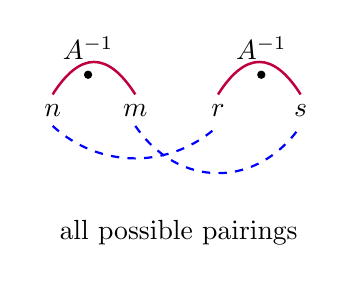
\begin{tikzpicture}[scale=1.0,baseline=(current bounding box.center)]
\node (n) at (0,0) {$n$};
\node (m) at (1.05,0) {$m$};
\node (r) at (2.1,0) {$r$};
\node (s) at (3.15,0) {$s$};
\fill (0.45,0.45) circle (1.5pt) node[above=2pt] {$A^{-1}$};
\fill (2.65,0.45) circle (1.5pt) node[above=2pt] {$A^{-1}$};
\draw[purple,line width=0.9pt] (n.north) .. controls (0.35,0.75) and (0.7,0.75) .. (m.north);
\draw[purple,line width=0.9pt] (r.north) .. controls (2.45,0.75) and (2.8,0.75) .. (s.north);
\draw[blue,dashed,line width=0.8pt] (n.south) .. controls (0.6,-0.75) and (1.5,-0.75) .. (r.south);
\draw[blue,dashed,line width=0.8pt] (m.south) .. controls (1.6,-1.0) and (2.6,-1.0) .. (s.south);
\node[text width=3.6cm,align=center] at (1.6,-1.55)
  {all possible pairings};
\end{tikzpicture}
\end{center}

There are $4!=24$ such terms before grouping, and the result is
\[
  \langle q_nq_mq_rq_s\rangle
  =
  (A^{-1})_{nm}(A^{-1})_{rs}
  +(A^{-1})_{nr}(A^{-1})_{ms}
  +(A^{-1})_{ns}(A^{-1})_{mr}.
\]
This is the Wick contraction rule:
\[
  \langle q_nq_mq_r\cdots\rangle
  =
  \sum_{\text{all inequivalent Wick contractions}}
  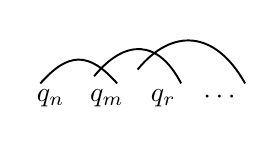
\begin{tikzpicture}[baseline=-0.55ex,scale=0.65]
    \node at (0,0) {$q_n$};
    \node at (1.1,0) {$q_m$};
    \node at (2.2,0) {$q_r$};
    \node at (3.3,0) {$\cdots$};
    \draw[line width=0.7pt] (-0.2,0.28) .. controls (0.35,0.9) and (0.75,0.9) .. (1.3,0.28);
    \draw[line width=0.7pt] (0.85,0.42) .. controls (1.45,1.15) and (2.1,1.15) .. (2.55,0.28);
    \draw[line width=0.7pt] (1.7,0.55) .. controls (2.35,1.35) and (3.2,1.35) .. (3.8,0.28);
  \end{tikzpicture},
\]
with
\[
  q_nq_m\ \hbox{contracted}\ :=\ (A^{-1})_{nm}.
\]

\subsection{Gaussian Functional Integrals}

Now generalize the Gaussian integral to a functional integral. In the following
formulas we set $\hbar=1$:
\[
  \vec q\longrightarrow q(\tau)
  \in
  \text{a linear space of real functions}
\]
with a suitable measure, and
\[
  \vec q\cdot\vec J
  \longrightarrow
  \int\dd\tau\,q(\tau)J(\tau).
\]
Consider the linear operator $A$,
\[
  A\cdot q(\tau):=\left(-\partial_\tau^2+\omega^2\right)q(\tau),
\]
and write its inverse as
\[
  A^{-1}\cdot g(\tau)
  =
  \int\dd\tau'\,G(\tau,\tau')g(\tau').
\]
The Green function obeys
\[
  \left(-\partial_\tau^2+\omega^2\right)G(\tau,\tau')
  =
  \delta(\tau-\tau').
\]
The Euclidean action is
\[
  S^E
  =
  \frac12(q,Aq)
  =
  \frac12\int\dd\tau\,q(\tau)\,A\cdot q(\tau),
\]
so
\[
  \langle q(\tau_1)q(\tau_2)\rangle
  =
  \frac{
    \int[\mathcal Dq]\,
    \ee^{-\frac12(q,Aq)}
    q(\tau_1)q(\tau_2)
  }{
    \int[\mathcal Dq]\,
    \ee^{-\frac12(q,Aq)}
  }.
\]

To avoid confusion with normalization in discretizing the integral in $\tau$,
we can obtain the answer using an integration-by-parts trick. Since
\[
  q(\tau_1)\ee^{-\frac12(q,Aq)}
  =
  -\left(A^{-1}\cdot\frac{\delta}{\delta q}\right)(\tau_1)
  \ee^{-\frac12(q,Aq)},
\]
we have
\[
\begin{aligned}
  &\int[\mathcal Dq]\,
  \ee^{-\frac12(q,Aq)}q(\tau_1)q(\tau_2)
  \\
  &\qquad =
  \int[\mathcal Dq]\,
  q(\tau_2)
  \left[
    -\left(A^{-1}\cdot\frac{\delta}{\delta q}\right)(\tau_1)
  \right]
  \ee^{-\frac12(q,Aq)}
  \\
  &\qquad =
  \int[\mathcal Dq]\,
  \ee^{-\frac12(q,Aq)}
  \left(A^{-1}\cdot\frac{\delta}{\delta q}\right)(\tau_1)
  q(\tau_2)
  \\
  &\qquad =
  \int[\mathcal Dq]\,
  \ee^{-\frac12(q,Aq)}
  \int\dd\tau'\,G(\tau_1,\tau')\delta(\tau'-\tau_2).
\end{aligned}
\]
Thus
\[
  \langle q(\tau_1)q(\tau_2)\rangle
  =
  G(\tau_1,\tau_2).
\]

Alternatively, work with the Fourier transformed variable
\[
  q(\tau)
  =
  \int_{-\infty}^{\infty}
  \frac{\dd k}{2\pi}\,\tilde q(k)\ee^{\ii k\tau},
  \qquad
  \tilde q^{\,*}(k)=\tilde q(-k).
\]
Then
\[
  A\cdot\tilde q(k)=(k^2+\omega^2)\tilde q(k),
  \qquad
  A^{-1}\cdot\tilde q(k)=\frac{1}{k^2+\omega^2}\tilde q(k).
\]
Therefore
\[
  G(\tau,\tau')
  =
  \int_{-\infty}^{\infty}
  \frac{\dd k}{2\pi}\,
  \frac{\ee^{\ii k(\tau-\tau')}}{k^2+\omega^2}
  =
  \frac{\ee^{-\omega|\tau-\tau'|}}{2\omega},
\]
in agreement with the earlier direct evaluation, having set $\hbar=1$.

Since $A$ is diagonal in the $\tilde q(k)$ basis,
\[
\begin{aligned}
  S^E
  &=
  \frac12(q,Aq)
  =
  \frac12\int_{-\infty}^{\infty}\dd\tau\,q(\tau)A\cdot q(\tau)
  \\
  &=
  \frac12
  \int_{-\infty}^{\infty}
  \frac{\dd k}{2\pi}\,
  \tilde q(-k)(k^2+\omega^2)\tilde q(k).
\end{aligned}
\]
Using the same integration-by-parts trick,
\[
  \langle \tilde q(k_1)\tilde q(k_2)\rangle
  =
  \frac{2\pi\delta(k_1+k_2)}{k_1^2+\omega^2}.
\]

\subsection{Anharmonic Oscillator}

Example 2 is the anharmonic oscillator,
\[
  H=\frac{p^2}{2}+\frac{q^2}{2}+\frac{g}{4!}q^4,
\]
or equivalently
\[
  L=\frac12\dot q^{\,2}-\frac{q^2}{2}-\frac{g}{4!}q^4.
\]
Study its spectrum using
\[
  \bra{0}\hat q(\tau)\hat q(0)\ket{0},
  \qquad
  \tau>0.
\]
By inserting a complete set of energy eigenstates,
\[
  \bra{0}\hat q(\tau)\hat q(0)\ket{0}
  =
  \sum_n
  \left|\bra{n}\hat q(0)\ket{0}\right|^2
  \ee^{-E_n\tau}.
\]
The same correlation function is represented by the Euclidean path integral
\[
  \bra{0}\hat q(\tau)\hat q(0)\ket{0}
  =
  \frac{1}{Z}
  \int[\mathcal Dq]\,
  \ee^{-\int\dd\tau\,L^E}
  q(\tau)q(0),
\]
where
\[
  Z=\int[\mathcal Dq]\,\ee^{-\int\dd\tau\,L^E},
  \qquad
  L^E=\frac12(\partial_\tau q)^2+\frac{q^2}{2}+\frac{g}{4!}q^4.
\]
Expand in powers of $g$:
\[
  Z
  =
  \int[\mathcal Dq]\,
  \ee^{-\int\dd\tau\left(\frac12(\partial_\tau q)^2+\frac12q^2\right)}
  \sum_{n=0}^{\infty}
  \frac{1}{n!}
  \left(
    -\frac{g}{4!}\int\dd\tau'\,q^4(\tau')
  \right)^n.
\]
At this stage one assumes that exchanging the order of the functional integral
and the expansion in $g$ is allowed; this point will be revisited later.

Let $Z_0$ denote the free Gaussian partition function. Then
\[
  \frac{Z_g}{Z_0}
  =
  \sum_{n=0}^{\infty}
  \frac{1}{n!}\left(-\frac{g}{4!}\right)^n
  \int \dd\tau_1\cdots \dd\tau_n\,
  \left\langle
    \bigl(q(\tau_1)\bigr)^4\cdots
    \bigl(q(\tau_n)\bigr)^4
  \right\rangle_0,
\]
where the expectation value is computed using the ``free'' Wick
contractions. For example, at order $g$,
\[
  -\frac{g}{4!}\int \dd\tau\,\left\langle q(\tau)^4\right\rangle_0
  =
  -\frac{g}{8}\int \dd\tau\,\bigl(G_0(\tau,\tau)\bigr)^2.
\]
Here $G_0(\tau,\tau)$ is a constant, so this expression diverges as the
range of $\tau$ is taken to infinity. We shall interpret this divergence
below.

At order $g^2$ one has
\[
  \frac{1}{2}\left(-\frac{g}{4!}\right)^2
  \int \dd\tau_1\,\dd\tau_2\,
  \left\langle \bigl(q(\tau_1)\bigr)^4\bigl(q(\tau_2)\bigr)^4
  \right\rangle_0.
\]
There are two types of Wick contractions:
\begin{center}
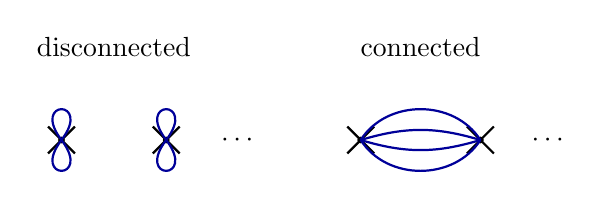
\begin{tikzpicture}[baseline=(current bounding box.center),scale=0.95]
  \node at (-1.0,1.25) {disconnected};
  \foreach \x in {-1.7,-0.3} {
    \draw[thick] (\x-0.18,-0.18) -- (\x+0.18,0.18);
    \draw[thick] (\x-0.18,0.18) -- (\x+0.18,-0.18);
    \fill (\x,0) circle (1.3pt);
    \draw[thick,blue!60!black]
      (\x,0) .. controls (\x-0.42,0.55) and (\x+0.42,0.55) .. (\x,0);
    \draw[thick,blue!60!black]
      (\x,0) .. controls (\x-0.42,-0.55) and (\x+0.42,-0.55) .. (\x,0);
  }
  \node at (0.65,0) {$\cdots$};

  \node at (3.1,1.25) {connected};
  \foreach \x in {2.3,3.9} {
    \draw[thick] (\x-0.18,-0.18) -- (\x+0.18,0.18);
    \draw[thick] (\x-0.18,0.18) -- (\x+0.18,-0.18);
    \fill (\x,0) circle (1.3pt);
  }
  \draw[thick,blue!60!black]
    (2.3,0) .. controls (2.65,0.55) and (3.55,0.55) .. (3.9,0);
  \draw[thick,blue!60!black]
    (2.3,0) .. controls (2.65,-0.55) and (3.55,-0.55) .. (3.9,0);
  \draw[thick,blue!60!black]
    (2.3,0) .. controls (2.9,0.18) and (3.3,0.18) .. (3.9,0);
  \draw[thick,blue!60!black]
    (2.3,0) .. controls (2.9,-0.18) and (3.3,-0.18) .. (3.9,0);
  \node at (4.8,0) {$\cdots$};
\end{tikzpicture}
\end{center}

More generally, at order $g^n$, each set of Wick contractions can be
represented by a graph. Suppose that the graph has $K$ connected components,
and that among them there are $m_\ell$ connected graphs containing
$\ell$ vertices each, for $\ell=1,2,3,\ldots$. Thus
\[
  \sum_{\ell\geq 1} m_\ell = K,
  \qquad
  \sum_{\ell\geq 1} \ell\,m_\ell = n.
\]
For a given partition of $n$, specified by the integers $m_\ell$, the
number of ways of grouping the $n$ vertices in this pattern is
\[
  \frac{n!}{\prod_{\ell\geq 1}(\ell!)^{m_\ell}m_\ell!}.
\]
If $G^{(\ell)}$ denotes the contribution from connected Wick contractions
of $\ell$ vertices, the total contribution of this partition is
\[
  \frac{1}{n!}\,
  \frac{n!}{\prod_{\ell\geq 1}(\ell!)^{m_\ell}m_\ell!}
  \prod_{\ell\geq 1}\bigl(G^{(\ell)}\bigr)^{m_\ell}
  =
  \prod_{\ell\geq 1}
  \frac{1}{m_\ell!}\left(\frac{1}{\ell!}G^{(\ell)}\right)^{m_\ell}.
\]
Summing over all $m_\ell$'s gives
\[
  \frac{Z_g}{Z_0}
  =
  \sum_{\{m_\ell\}}
  \prod_{\ell\geq 1}
  \frac{1}{m_\ell!}\left(\frac{1}{\ell!}G^{(\ell)}\right)^{m_\ell}
  =
  \prod_{\ell\geq 1}\exp\left(\frac{1}{\ell!}G^{(\ell)}\right)
  =
  \exp\left(\sum_{\ell\geq 1}\frac{1}{\ell!}G^{(\ell)}\right).
\]
Thus the logarithm of the partition function is the contribution from all
connected graphs.

As an example, one connected graph with three vertices contributes
\[
\begin{tikzpicture}[baseline=-0.45ex,scale=0.85]
  \coordinate (a) at (0,0);
  \coordinate (b) at (1.5,0);
  \coordinate (c) at (0.75,1.1);
  \foreach \p in {a,b,c} {
    \draw[thick] ($(\p)+(-0.15,-0.15)$) -- ($(\p)+(0.15,0.15)$);
    \draw[thick] ($(\p)+(-0.15,0.15)$) -- ($(\p)+(0.15,-0.15)$);
    \fill (\p) circle (1.2pt);
  }
  \draw[thick,blue!60!black] (a) .. controls (0.55,0.24) and (0.95,0.24) .. (b);
  \draw[thick,blue!60!black] (a) .. controls (0.55,-0.24) and (0.95,-0.24) .. (b);
  \draw[thick,blue!60!black] (b) .. controls (1.25,0.55) and (1.1,0.9) .. (c);
  \draw[thick,blue!60!black] (b) .. controls (1.55,0.65) and (1.25,1.15) .. (c);
  \draw[thick,blue!60!black] (c) .. controls (0.5,0.9) and (0.25,0.55) .. (a);
  \draw[thick,blue!60!black] (c) .. controls (-0.05,1.15) and (-0.15,0.65) .. (a);
\end{tikzpicture}
\quad
=
\frac{1}{3!}\left(-\frac{g}{4!}\right)^3
\int \dd\tau_1\,\dd\tau_2\,\dd\tau_3\,
\bigl(G_0(\tau_1,\tau_2)\bigr)^2
\bigl(G_0(\tau_2,\tau_3)\bigr)^2
\bigl(G_0(\tau_3,\tau_1)\bigr)^2.
\]
This still diverges like $\int\dd\tau$ times a constant.

\subsection{Ground State Energy from Vacuum Diagrams}

The interpretation of
\[
  Z=\int [\mathcal Dq]\,e^{-\int\dd\tau\,L^E}
\]
is
\[
  Z=\bra{q_f}e^{-HT}\ket{q_i},
\]
with boundary conditions at the initial and final imaginary times
$\tau=0,T$. Since these boundary conditions become unimportant as
$T\to\infty$,
\[
  \log Z=-E_0T+O(1),
\]
where $E_0$ is the ground-state energy. Indeed, perturbation theory gave
\[
  \log\left(\frac{Z_g}{Z_0}\right)
  =
  \sum_{\ell=1}^{\infty}\frac{1}{\ell!}G^{(\ell)},
\]
the sum of all connected Wick contractions of $\ell$ vertices.

One often absorbs the combinatorical factor $1/\ell!$ into the symmetry
factor of the graph itself. Each $G^{(\ell)}$ is of the form
$\int\dd\tau\,(\text{const.})$, and therefore is proportional to $T$.
Thus
\[
  E_0=-\lim_{T\to\infty}\frac{1}{T}\log Z
\]
is well-defined.

As already seen, at order $g$, $\ell=1$. The connected vacuum graph is
\[
  G^{(1)}
  =
  3\,
  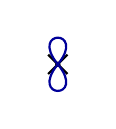
\begin{tikzpicture}[baseline=-0.5ex,scale=0.82]
    \draw[thick] (-0.15,-0.15) -- (0.15,0.15);
    \draw[thick] (-0.15,0.15) -- (0.15,-0.15);
    \fill (0,0) circle (1.2pt);
    \draw[thick,blue!60!black]
      (0,0) .. controls (-0.45,0.55) and (0.45,0.55) .. (0,0);
    \draw[thick,blue!60!black]
      (0,0) .. controls (-0.45,-0.55) and (0.45,-0.55) .. (0,0);
  \end{tikzpicture}
  =
  -\frac{g}{8}\int\dd\tau\,\bigl(G_0(\tau,\tau)\bigr)^2.
\]
Recall that
\[
  G_0(\tau_1,\tau_2)=\frac{1}{2\omega}e^{-\omega|\tau_{12}|},
  \qquad
  G_0(\tau,\tau)=\frac{1}{2\omega}.
\]
Thus, setting $\omega=1$ when desired,
\[
  \Delta E_0
  =
  \frac{g}{8}\left(\frac{1}{2\omega}\right)^2+O(g^2).
\]

This agrees with Hamiltonian perturbation theory. Writing
\[
  H=
  \underbrace{\frac{\hat p^2}{2}+\frac{\hat q^2}{2}}_{H_0}
  +
  \underbrace{\frac{g}{4!}\hat q^4}_{H_1},
\]
and letting $\ket{\psi_0}$ be the ground state of $H_0$, to leading order
in $g$,
\[
  \Delta E_0\simeq
  \bra{\psi_0}H_1\ket{\psi_0}
  =
  \frac{g}{4!}\left\langle q^4\right\rangle_0
  =
  \frac{g}{4!}\cdot\frac{3}{4}
  =
  \frac{g}{32}.
\]

\subsection{The Two-Point Function and One-Particle-Irreducible Graphs}

\newcommand{\qftFreeProp}{%
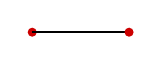
\begin{tikzpicture}[baseline=-0.55ex,scale=0.82]
  \fill[red!80!black] (0,0) circle (2pt);
  \draw[thick] (0,0) -- (1.5,0);
  \fill[red!80!black] (1.5,0) circle (2pt);
\end{tikzpicture}}
\newcommand{\qftTadpoleProp}{%
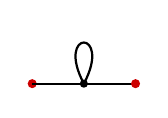
\begin{tikzpicture}[baseline=-0.55ex,scale=0.82]
  \fill[red!80!black] (0,0) circle (2pt);
  \draw[thick] (0,0) -- (1.6,0);
  \fill[red!80!black] (1.6,0) circle (2pt);
  \fill (0.8,0) circle (1.8pt);
  \draw[thick] (0.8,0) .. controls (0.35,0.85) and (1.25,0.85) .. (0.8,0);
\end{tikzpicture}}
\newcommand{\qftDoubleTadpoleProp}{%
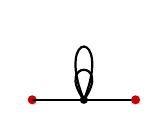
\begin{tikzpicture}[baseline=-0.55ex,scale=0.82]
  \fill[red!80!black] (0,0) circle (2pt);
  \draw[thick] (0,0) -- (1.6,0);
  \fill[red!80!black] (1.6,0) circle (2pt);
  \fill (0.8,0) circle (1.8pt);
  \draw[thick] (0.8,0) .. controls (0.35,0.62) and (1.25,0.62) .. (0.8,0);
  \draw[thick] (0.8,0) .. controls (0.35,1.1) and (1.25,1.1) .. (0.8,0);
\end{tikzpicture}}
\newcommand{\qftTwoVertexTadpoles}{%
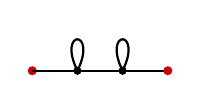
\begin{tikzpicture}[baseline=-0.55ex,scale=0.82]
  \fill[red!80!black] (0,0) circle (2pt);
  \draw[thick] (0,0) -- (2.1,0);
  \fill[red!80!black] (2.1,0) circle (2pt);
  \foreach \x in {0.7,1.4} {
    \fill (\x,0) circle (1.8pt);
    \draw[thick] (\x,0) .. controls (\x-0.32,0.65) and (\x+0.32,0.65) .. (\x,0);
  }
\end{tikzpicture}}
\newcommand{\qftBubbleProp}{%
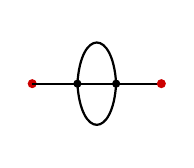
\begin{tikzpicture}[baseline=-0.55ex,scale=0.82]
  \fill[red!80!black] (0,0) circle (2pt);
  \draw[thick] (0,0) -- (2.0,0);
  \fill[red!80!black] (2.0,0) circle (2pt);
  \fill (0.7,0) circle (1.8pt);
  \fill (1.3,0) circle (1.8pt);
  \draw[thick] (0.7,0) .. controls (0.75,0.85) and (1.25,0.85) .. (1.3,0);
  \draw[thick] (0.7,0) .. controls (0.75,-0.85) and (1.25,-0.85) .. (1.3,0);
\end{tikzpicture}}
\newcommand{\qftBlobProp}{%
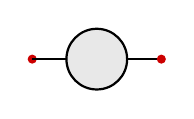
\begin{tikzpicture}[baseline=-0.55ex,scale=0.82]
  \fill[red!80!black] (0,0) circle (2pt);
  \draw[thick] (0,0) -- (0.55,0);
  \draw[fill=gray!18,thick] (1.0,0) circle (0.47);
  \draw[thick] (1.45,0) -- (2.0,0);
  \fill[red!80!black] (2.0,0) circle (2pt);
\end{tikzpicture}}
\newcommand{\qftOnePI}{%
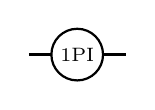
\begin{tikzpicture}[baseline=-0.55ex,scale=0.82]
  \draw[thick] (0,0) -- (0.35,0);
  \draw[thick] (1.15,0) -- (1.5,0);
  \draw[thick] (0.75,0) circle (0.4);
  \node at (0.75,0) {\scriptsize 1PI};
\end{tikzpicture}}
\newcommand{\qftOnePIChain}{%
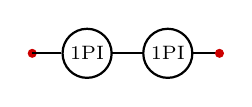
\begin{tikzpicture}[baseline=-0.55ex,scale=0.82]
  \fill[red!80!black] (0,0) circle (2pt);
  \draw[thick] (0,0) -- (0.45,0);
  \draw[thick] (0.85,0) circle (0.38);
  \node at (0.85,0) {\scriptsize 1PI};
  \draw[thick] (1.23,0) -- (1.72,0);
  \draw[thick] (2.1,0) circle (0.38);
  \node at (2.1,0) {\scriptsize 1PI};
  \draw[thick] (2.48,0) -- (2.9,0);
  \fill[red!80!black] (2.9,0) circle (2pt);
\end{tikzpicture}}

Next we turn to
\[
  \bra{0}\hat q(\tau)\hat q(0)\ket{0},
  \qquad \tau>0,
\]
which is
\[
  \frac{1}{Z}\int[\mathcal Dq]\,
  e^{-\int\dd\tau\,L^E}\,q(\tau)q(0).
\]
Expanding in \(g\),
\[
  \bra{0}\hat q(\tau)\hat q(0)\ket{0}
  =
  \frac{1}{Z}
  \left\langle
    q(\tau)q(0)
    \sum_{n=0}^{\infty}
    \frac{1}{n!}
    \left(
      -\frac{g}{4!}\int\dd\tau'\,q^4(\tau')
    \right)^n
  \right\rangle_0.
\]
This is computed by summing all possible Wick contractions. A typical term
has one connected component containing the external insertions, together
with other disconnected components:
\begin{center}
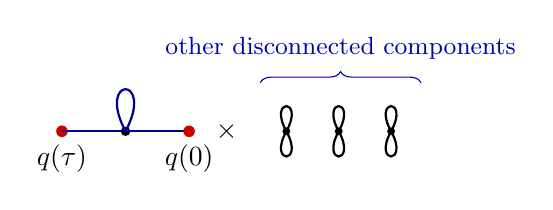
\begin{tikzpicture}[scale=0.95]
  \fill[red!80!black] (0,0) circle (2.2pt);
  \node[below] at (0,-0.05) {$q(\tau)$};
  \draw[thick,blue!60!black] (0,0) -- (0.85,0);
  \fill (0.85,0) circle (1.8pt);
  \draw[thick,blue!60!black] (0.85,0) .. controls (0.45,0.75) and (1.25,0.75) .. (0.85,0);
  \draw[thick,blue!60!black] (0.85,0) -- (1.7,0);
  \fill[red!80!black] (1.7,0) circle (2.2pt);
  \node[below] at (1.7,-0.05) {$q(0)$};
  \node at (2.2,0) {$\times$};
  \draw[decorate,decoration={brace,amplitude=4pt},blue!70!black]
    (2.65,0.65) -- (4.8,0.65)
    node[midway,above=5pt] {\small other disconnected components};
  \foreach \x in {3.0,3.7,4.4} {
    \draw[thick] (\x,0) .. controls (\x-0.25,0.45) and (\x+0.25,0.45) .. (\x,0);
    \draw[thick] (\x,0) .. controls (\x-0.25,-0.45) and (\x+0.25,-0.45) .. (\x,0);
    \fill (\x,0) circle (1.5pt);
  }
\end{tikzpicture}
\end{center}
The sum factorizes into a connected graph joining \(q(\tau)\) to \(q(0)\)
times disconnected vacuum graphs. The disconnected vacuum graphs cancel
against the factor \(1/Z\), leaving
\[
  \bra{0}\hat q(\tau)\hat q(0)\ket{0}
  =
  \qftFreeProp
  \;+\;
  \qftTadpoleProp
  \;+\;
  \qftTwoVertexTadpoles
  \;+\;
  \qftDoubleTadpoleProp
  \;+\;
  \qftBubbleProp
  \;+\;\cdots .
\]

The same path integral expression computes
\(\bra{0}\hat q(0)\hat q(\tau)\ket{0}\) for \(\tau<0\). We can write the
Euclidean Green function as
\[
  G_E(\tau)=\langle q(\tau)q(0)\rangle
  =
  \begin{cases}
    \bra{0}\hat q(\tau)\hat q(0)\ket{0}, & \tau>0,\\
    \bra{0}\hat q(0)\hat q(\tau)\ket{0}, & \tau<0.
  \end{cases}
\]
At zeroth order,
\[
  \qftFreeProp
  =
  G_0(\tau)
  =
  \frac{1}{2}e^{-|\tau|}
  =
  \int\frac{\dd k}{2\pi}\,\widetilde G_0(k)e^{ik\tau},
  \qquad
  \widetilde G_0(k)=\frac{1}{k^2+1}.
\]
At order \(g\), the connected correction is
\[
  \qftTadpoleProp
  =
  -\frac{g}{2}
  \int\dd\tau'\,
  G_0(\tau-\tau')G_0(\tau')G_0(0).
\]
It is convenient to evaluate this using the Fourier transform:
\[
\begin{aligned}
  \qftTadpoleProp
  &=
  -\frac{g}{2}
  \int\dd\tau'
  \int\frac{\dd k}{2\pi}\frac{\dd k'}{2\pi}\frac{\dd k''}{2\pi}\,
  \widetilde G_0(k)\widetilde G_0(k')\widetilde G_0(k'')\,
  e^{ik(\tau-\tau')+ik'\tau'}                                      \\
  &=
  -\frac{g}{2}\cdot\frac{1}{2}
  \int\frac{\dd k}{2\pi}\,
  \frac{e^{ik\tau}}{(k^2+1)^2}.
\end{aligned}
\]
At order \(g^2\), the diagrams
\[
  \qftTwoVertexTadpoles
  \qquad
  \qftDoubleTadpoleProp
  \qquad
  \qftBubbleProp
\]
are left as a Problem Set 2 calculation.

The full perturbative two-point function has the structure
\[
  \qftBlobProp
  =
  \qftFreeProp
  \;+\;
  \qftOnePI
  \;+\;
  \qftOnePIChain
  \;+\;\cdots .
\]
Here ``1PI'' means one-particle-irreducible: the graph remains connected
after cutting any one propagator. In momentum space this gives
\[
  G(\tau)
  =
  \int\frac{\dd k}{2\pi}\,e^{ik\tau}\,
  \widetilde G_0(k)
  \sum_{n=0}^{\infty}\bigl(\widetilde G_0(k)\Sigma(k)\bigr)^n
  =
  \int\frac{\dd k}{2\pi}\,e^{ik\tau}\,
  \frac{1}{k^2+1-\Sigma(k)}.
\]
The self-energy \(\Sigma(k)\) is the sum of amputated 1PI graphs, not
including the external propagators. To second order,
\[
  \Sigma(k)
  =
  -\frac{g}{4}
  +
  \frac{g^2}{8}
  \left(
    \frac{1}{4}+\frac{1}{k^2+9}
  \right)
  +O(g^3).
\]
Therefore
\[
  \langle q(\tau)q(0)\rangle
  \equiv G(\tau)
  =
  \int\frac{\dd k}{2\pi}\,\widetilde G(k)e^{ik\tau},
\]
with
\[
  \widetilde G(k)
  =
  \frac{1}{
    k^2+1+\frac{g}{4}
    -\frac{g^2}{8}\left(\frac{1}{4}+\frac{1}{k^2+9}\right)
    +O(g^3)
  }.
\]

On the other hand, for \(\tau>0\) we know that
\[
  \bra{0}\hat q(\tau)\hat q(0)\ket{0}
  =
  \sum_n
  \left|\bra{n}\hat q(0)\ket{0}\right|^2
  e^{-(E_n-E_0)\tau}.
\]
Consider the analytic continuation of \(\widetilde G(k)\) to the complex
\(k\)-plane:
\begin{center}
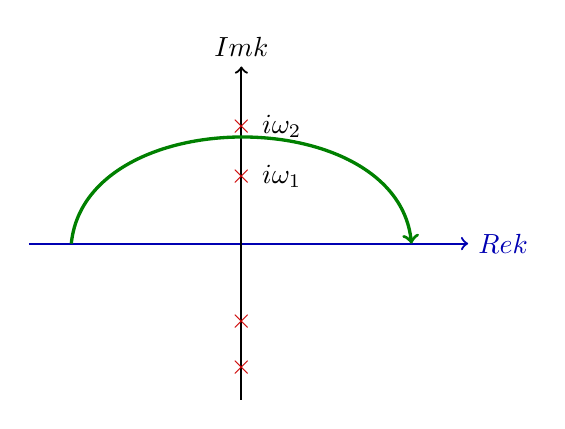
\begin{tikzpicture}[scale=0.9]
  \draw[->,thick,blue!70!black] (-3.0,0) -- (3.2,0) node[right] {$\operatorname{Re}k$};
  \draw[->,thick] (0,-2.2) -- (0,2.5) node[above] {$\operatorname{Im}k$};
  \draw[very thick,green!50!black,->]
    (-2.4,0) .. controls (-2.2,2.0) and (2.2,2.0) .. (2.4,0);
  \foreach \y/\lab in {0.95/{i\omega_1},1.65/{i\omega_2}} {
    \node[red!80!black] at (0,\y) {$\times$};
    \node[right=4pt] at (0,\y) {$\lab$};
  }
  \node[red!80!black] at (0,-1.1) {$\times$};
  \node[red!80!black] at (0,-1.75) {$\times$};
\end{tikzpicture}
\end{center}
Closing the contour at infinity in the upper half-plane,
\[
  \int\frac{\dd k}{2\pi}\,\widetilde G(k)e^{ik\tau}
  =
  i\sum_n e^{-\omega_n\tau}
  \operatorname*{Res}_{k\to i\omega_n}\widetilde G(k),
  \qquad
  \omega_n=E_n-E_0.
\]
For example, from the expression above for \(\widetilde G(k)\), the first
pole is expected near \(k\simeq i\), and one finds
\[
  \omega_1
  =
  1+\frac{g}{8}-\frac{g^2}{32}+O(g^3),
\]
which agrees with Hamiltonian perturbation theory at second order.

\subsection{Derivative Interactions and the Measure}

Here is a closely related example which is more subtle. Take
\[
  L=\frac12\dot q^2-\frac12 q^2-\frac{g}{8}q^2\dot q^2 .
\]
The canonical momentum is
\[
  p=\frac{\partial L}{\partial \dot q}
    =\dot q\left(1-\frac{g}{4}q^2\right),
\]
and therefore
\[
  H=\dot q p-L
   =\frac12\left(1-\frac{g}{4}q^2\right)^{-1}p^2+\frac12q^2 .
\]
This expression already suggests a possible operator-ordering ambiguity in
quantization.

One can also consider a change of variable
\[
  \dot y=\left(1-\frac{g}{4}q^2\right)^{1/2}\dot q,
  \qquad
  y=q-\frac{g}{24}q^3+\cdots .
\]
In terms of the new variable the Lagrangian takes the form
\[
  L=\frac12\dot y^2-V(y),
  \qquad
  V(y)=\frac12 y^2+\frac{g}{24}y^4+\cdots ,
\]
which is the anharmonic oscillator up to corrections of order \(g^2\) in the
potential. We will instead insist on working with the \(q\)-variable in the
path integral and see what happens.

The Euclidean Lagrangian is
\[
  L^E
  =\frac12(\partial_\tau q)^2+\frac12q^2
    -\frac{g}{8}q^2(\partial_\tau q)^2 .
\]
It is useful to write the interaction term as
\[
  q^2(\partial_\tau q)^2
  =\frac13\,\partial_\tau\!\left(q^3\partial_\tau q\right)
    -\frac13\,q^3\partial_\tau^2q,
\]
so that, up to a total derivative,
\[
  L^E
  =\frac12(\partial_\tau q)^2+\frac12q^2
    +\frac{g}{24}q^3\partial_\tau^2q .
\]

To first order in \(g\), the two-point function is
\[
\begin{aligned}
  \langle q(\tau)q(0)\rangle
  &=G_0(\tau)
    +\frac{g}{8}\int \dd \tau'\,
      \big\langle q(\tau)q(0)\,q(\tau')^2
      \big(\partial_{\tau'}q(\tau')\big)^2\big\rangle_0+\cdots .
\end{aligned}
\]
The possible Wick contractions are represented schematically by
\[
\begin{tikzpicture}[baseline=(current bounding box.center), x=1cm, y=1cm]
  \coordinate (a) at (0,0);
  \coordinate (b) at (1.2,0);
  \coordinate (c) at (2.4,0);
  \draw (a) node[below] {\(\tau\)};
  \draw (c) node[below] {\(0\)};
  \draw (a) -- (b) -- (c);
  \draw (b) circle[radius=.28];
  \draw[blue, thick] ($(b)+(-.08,.28)$) -- ($(b)+(-.08,.48)$);
  \draw[blue, thick] ($(b)+(.08,.28)$) -- ($(b)+(.08,.48)$);
  \node at (b) [below=.38cm] {\(\tau'\)};

  \node at (3.1,0) {\(+\)};

  \coordinate (d) at (3.8,0);
  \coordinate (e) at (5.0,0);
  \coordinate (f) at (6.2,0);
  \draw (d) -- (e) -- (f);
  \draw (e) circle[radius=.28];
  \draw[blue, thick] ($(e)+(-.22,.15)$) -- ($(e)+(-.35,.32)$);
  \draw[blue, thick] ($(e)+(.22,.15)$) -- ($(e)+(.35,.32)$);
  \node at (e) [below=.38cm] {\(\tau'\)};

  \node at (6.9,0) {\(+\)};

  \coordinate (g) at (7.6,0);
  \coordinate (h) at (8.8,0);
  \coordinate (i) at (10.0,0);
  \draw (g) -- (h) -- (i);
  \draw (h) .. controls +(70:.55) and +(110:.55) .. (h);
  \draw[blue, thick] ($(h)+(-.18,.2)$) -- ($(h)+(-.35,.38)$);
  \draw[blue, thick] ($(h)+(.18,.2)$) -- ($(h)+(.35,.38)$);
  \node at (h) [below=.38cm] {\(\tau'\)};

  \node at (10.7,0) {\(+\cdots\)};
\end{tikzpicture}
\]
where the blue marks indicate derivatives acting on the corresponding
propagators.

One of these terms gives
\[
  2\cdot\frac{g}{8}\int\dd\tau'\,
  G_0(\tau-\tau')G_0(\tau')\,\bigl(-\partial^2G_0(0)\bigr)
  =
  \frac{g}{4}\int\dd\tau'\,
  G_0(\tau-\tau')G_0(\tau')\,\bigl(-\partial^2G_0(0)\bigr).
\]
Since
\[
  G_0(\tau)=\frac12e^{-|\tau|},
\]
the factor \(-\partial^2G_0(0)\) is divergent. The other contributions are
finite. For example,
\[
  \frac{g}{4}
  \int\frac{\dd k}{2\pi}\,
    \frac{e^{ik\tau}}{(k^2+1)^2}\,k^2
  \int\frac{\dd k'}{2\pi}\,\frac{1}{k'^2+1},
\]
and
\[
  -\frac{g}{2}
  \int\frac{\dd k}{2\pi}\,
    \frac{e^{ik\tau}}{(k^2+1)^2}\,ik
  \int\frac{\dd k'}{2\pi}\,\frac{ik'}{k'^2+1}=0
\]
by symmetry. The remaining diagrams are similar.

The divergence comes from the integral at large momentum. Its origin lies in
the definition of the path integral measure. Writing
\[
  q(\tau)=\int\frac{\dd k}{2\pi}\,\widetilde q(k)e^{ik\tau},
\]
the formal measure is
\[
  [Dq]=\prod_k \dd \widetilde q_k .
\]
To define it, introduce a cutoff
\[
  [Dq]_\Lambda=\prod_{|k|<\Lambda}\dd \widetilde q_k .
\]
This cuts off the loop integral by \(|k'|<\Lambda\); only after computing do
we ask whether \(\Lambda\to\infty\) can be taken.

With this regularization,
\[
  \widetilde G(k)
  =\frac{1}{k^2+1-\Sigma(k)} ,
\]
and, to first order in \(g\),
\[
\begin{aligned}
  \Sigma_\Lambda(k)
  &=
  \frac{g}{4}\int_{|k'|<\Lambda}
       \frac{\dd k'}{2\pi}\,\frac{k'^2}{k'^2+1}
  +\frac{g}{4}k^2
       \int_{|k'|<\Lambda}
       \frac{\dd k'}{2\pi}\,\frac{1}{k'^2+1}
  +O(g^2)\\
  &=
  \frac{g}{4}\left(
    \frac{\Lambda}{\pi}+\frac{k^2}{2}-\frac12+O(\Lambda^{-1})
  \right)+O(g^2).
\end{aligned}
\]

What is the interpretation of the \(\Lambda\to\infty\) limit? There is
nothing wrong with the quantum-mechanical Hamiltonian
\[
  H=\frac12\left(1-\frac{g}{4}q^2\right)^{-1}p^2+\frac12q^2
\]
at least for \(g<0\), aside from the operator-ordering ambiguity mentioned
above. To understand what is going on, restore the \(\hbar\)-dependence:
\[
  Z=\int[Dq]\,
  \exp\left[-\frac{1}{\hbar}\int\dd\tau\,L^E\right].
\]
Then
\[
  \widetilde G(k)=\frac{\hbar}{k^2+1-\Sigma(k)}
\]
and
\[
  \Sigma_\Lambda(k)
  =\frac{\hbar g}{4}\left(
    \frac{\Lambda}{\pi}+\frac{k^2}{2}-\frac12+O(\Lambda^{-1})
  \right)+O(\hbar^2g^2).
\]

Indeed, if we include a counterterm
\[
  \Delta L^E=C\,g\,\hbar\,\frac{q^2}{2},
\]
the one-particle-irreducible two-point function receives an extra
contribution \(-C g\hbar\). Thus
\[
  \Sigma_\Lambda(k)
  =
  \hbar g\left(
    \frac{k^2}{8}+\frac{\Lambda}{4\pi}
    -\frac18-C+O(\Lambda^{-1})
  \right)+O(g^2).
\]
The path integral is only defined once a regularization has been specified.
Choosing
\[
  C=\frac{\Lambda}{4\pi}+\text{finite}
\]
and taking \(\Lambda\to\infty\) at the end gives a finite answer for
\(\Sigma(k)\). The finite part of \(C\) represents an ambiguity in
quantization, namely the possibility of adjusting the quantum Hamiltonian by a
term of order \(\hbar\).

The pole of
\[
  \widetilde G(k)=\frac{\hbar}{k^2+1-\Sigma(k)}
\]
at \(k=i\omega_1\) gives
\[
  \omega_1
  =
  1+\hbar g\left(
    -\frac{\Lambda}{8\pi}+\frac{C}{2}+\frac18
  \right)+O(g^2)
  =E_1-E_0 .
\]
This energy gap is an unambiguous physical observable, regardless of the
interpretation of \(q(\tau)\). The counterterms, together with the
regularization scheme, should be viewed as part of the definition of the path
integral. Fixing the finite part of the counterterms requires additional
physical input, for example symmetries of the quantum Hamiltonian. In general
quantum mechanics anything can appear in \(H\); in quantum field theory,
Poincare symmetry and causality are highly restrictive.

\section{A Manifestly Relativistic Theory of Fields}

In classical mechanics the dynamical variables are \(q^i(t)\). In a field
theory they are replaced by fields
\[
  q^i(t)\quad\leadsto\quad \phi(t,\vec x),
\]
where \(\vec x\in \mathbb R^{D-1}\) is viewed as a continuous label for the
variables. We will write
\[
  x^\mu=(x^0,\vec x),\qquad x^0=t,
\]
interchangeably.

The action is
\[
  S=\int \dd t\,\dd^{D-1}\vec x\,
  \mathcal L\bigl[\phi(x),\partial_\mu\phi(x),\ldots\bigr]
  =
  \int \dd^D x\,
  \mathcal L\bigl[\phi(x),\partial_\mu\phi(x),\ldots\bigr],
\]
where \(\mathcal L\) is the Lagrangian density. The equation of motion is
\[
  \frac{\delta S}{\delta\phi(x)}=0.
\]
Assume for now that \(\mathcal L\) depends on \(\phi(x)\) only through
\(\phi(x)\) and its first-order derivatives \(\partial_\mu\phi(x)\). Then
\[
\begin{aligned}
  \delta S
  &=
  \int\dd^D x\left[
    \delta\phi(x)\frac{\partial\mathcal L}{\partial\phi(x)}
    +\delta\partial_\mu\phi(x)
      \frac{\partial\mathcal L}{\partial(\partial_\mu\phi(x))}
  \right]\\
  &=
  \int\dd^D x\,\delta\phi(x)\left[
    \frac{\partial\mathcal L}{\partial\phi(x)}
    -\partial_\mu
      \frac{\partial\mathcal L}{\partial(\partial_\mu\phi(x))}
  \right],
\end{aligned}
\]
where the second line follows by integration by parts. The Euler-Lagrange
equation is therefore
\[
  \frac{\partial\mathcal L}{\partial\phi(x)}
  -\partial_\mu
   \frac{\partial\mathcal L}{\partial(\partial_\mu\phi(x))}
  =0 .
\]

\subsection{The Free Massive Scalar Field}

For a free massive scalar field,
\[
  \mathcal L
  =
  \frac12(\partial_t\phi)^2
  -\frac12\sum_{i=1}^{D-1}(\partial_{x^i}\phi)^2
  -\frac12m^2\phi^2 .
\]
With the convention
\[
  \eta^{\mu\nu}=\operatorname{diag}(-1,1,\ldots,1),
\]
this can be written as
\[
  \mathcal L
  =
  -\frac12(\partial_\mu\phi)^2-\frac12m^2\phi^2 .
\]
The Euler-Lagrange equation gives the Klein-Gordon equation
\[
  \partial^\mu\partial_\mu\phi-m^2\phi=0 .
\]

The general solution can be written as a Fourier transform
\[
  \phi(x)=\int \dd^D k\, f(k)e^{ik\cdot x}.
\]
Using
\[
  k\cdot x=\vec k\cdot\vec x-k^0x^0,
\]
the equation of motion requires
\[
  (k^2+m^2)f(k)=0.
\]
Thus \(f(k)\) is a distribution supported on the mass shell
\[
  k^2+m^2=0,
  \qquad
  k^0=\pm\sqrt{\vec k^2+m^2}.
\]
Equivalently,
\[
  \phi(x)
  =
  \int \dd^{D-1}\vec k\,
  \left[
    \widetilde f(\vec k)\,
      e^{i\vec k\cdot\vec x-i\omega_{\vec k}x^0}
    +
    \widetilde f^*(\vec k)\,
      e^{-i\vec k\cdot\vec x+i\omega_{\vec k}x^0}
  \right],
\]
where
\[
  \omega_{\vec k}=\sqrt{\vec k^2+m^2}.
\]

The initial-value problem is: given
\(\phi(t=0,\vec x)\) and \(\partial_t\phi(t=0,\vec x)\), determine
\(\phi(t>0,\vec x)\). At \(t=0\),
\[
  \phi(t=0,\vec x)
  =
  \int\dd^{D-1}\vec k\,e^{i\vec k\cdot\vec x}
  \left[
    \widetilde f(\vec k)+\widetilde f^*(-\vec k)
  \right],
\]
and
\[
  \partial_t\phi(t=0,\vec x)
  =
  \int\dd^{D-1}\vec k\,e^{i\vec k\cdot\vec x}
  (-i\omega_{\vec k})
  \left[
    \widetilde f(\vec k)-\widetilde f^*(-\vec k)
  \right].
\]
Together these determine \(\widetilde f(\vec k)\) and
\(\widetilde f^*(-\vec k)\), and hence \(\phi(x)\) at any time
\(t\equiv x^0\).

A relativistic quantum theory may be constructed by quantizing the classical
field theory. There are two approaches.

\begin{enumerate}[label=(\arabic*)]
\item Canonical quantization: construct a Hilbert space using wave functions
  in the variables \(\phi(\vec x,t=0)\), together with the Hamiltonian \(H\).
\item Path integral:
  \[
    Z=\int[D\phi]\,
    e^{\frac{i}{\hbar}S[\phi]} .
  \]
  To make sense of the functional measure typically requires regularization.
\end{enumerate}

\subsection{Canonical Formalism}

The Lagrangian is
\[
  L=\int\dd^{D-1}\vec x\,
  \mathcal L[\phi,\partial_\mu\phi].
\]
For the free scalar field,
\[
  L=\int\dd^{D-1}\vec x\,
  \left[
    -\frac12(\partial_\mu\phi)^2-\frac12m^2\phi^2
  \right].
\]
The dynamical variable is \(\phi(t,\vec x)\). The time \(t\) is the evolution
parameter, while \(\vec x\) is just a continuous label. Thus the canonical
coordinates are the values of \(\phi(t,\vec x)\).

The conjugate canonical momentum density is
\[
  \Pi(t,\vec x)
  =
  \frac{\partial\mathcal L}{\partial\dot\phi(t,\vec x)}
  =
  \dot\phi(t,\vec x)
\]
in the present example. The classical Hamiltonian is
\[
  H=\int\dd^{D-1}\vec x\,\mathcal H,
\]
with Hamiltonian density
\[
  \mathcal H
  =
  \Pi(t,\vec x)\dot\phi(t,\vec x)-\mathcal L.
\]
For the free scalar field,
\[
  \mathcal H
  =
  \frac12\dot\phi^2+\frac12(\partial_{\vec x}\phi)^2+\frac12m^2\phi^2
  =
  \frac12\Pi^2+\frac12(\partial_{\vec x}\phi)^2+\frac12m^2\phi^2.
\]
In terms of \((\phi,\Pi)\), the \(\Pi^2\) term is kinetic and the remaining
terms are potential.

Omitting the time argument, the Poisson brackets are
\[
  \{\phi(\vec x),\phi(\vec x')\}=0=\{\Pi(\vec x),\Pi(\vec x')\},
\]
and
\[
  \{\Pi(\vec x),\phi(\vec x')\}
  =\delta^{D-1}(\vec x-\vec x').
\]
For two functionals,
\[
  \{F,G\}
  =
  \int\dd^{D-1}\vec x\left[
    \frac{\delta F}{\delta\Pi(\vec x)}
    \frac{\delta G}{\delta\phi(\vec x)}
    -
    \frac{\delta F}{\delta\phi(\vec x)}
    \frac{\delta G}{\delta\Pi(\vec x)}
  \right].
\]
The equations of motion are
\[
  \dot F=\{H,F\}
\]
as usual.

Quantization promotes \(\phi(t,\vec x)\) and \(\Pi(t,\vec x)\) to operators
\[
  \hat\phi(t,\vec x),\qquad \hat\Pi(t,\vec x),
\]
which obey equal-time commutators
\[
  [\hat\phi(t,\vec x),\hat\phi(t,\vec x')]
  =0=
  [\hat\Pi(t,\vec x),\hat\Pi(t,\vec x')],
\]
and
\[
  [\hat\phi(t,\vec x),\hat\Pi(t,\vec x')]
  =
  i\hbar\,\delta^{D-1}(\vec x-\vec x').
\]

It is convenient to perform a spatial Fourier transform, say at \(t=0\):
\[
  \hat\phi(t=0,\vec x)
  =
  \int
  \frac{\dd^{D-1}\vec k}
  {\sqrt{(2\pi)^{D-1}2\nu(\vec k)}}\,
  \bigl(a_{\vec k}+a^\dagger_{-\vec k}\bigr)
  e^{i\vec k\cdot\vec x}.
\]
For now the denominator is just a normalization convention, and the
combination \(a_{\vec k}+a^\dagger_{-\vec k}\) can be viewed as a definition
of the \(a\)'s. Similarly,
\[
  \hat\Pi(t=0,\vec x)
  =
  \int
  \frac{\dd^{D-1}\vec k}
  {\sqrt{(2\pi)^{D-1}2\nu(\vec k)}}\,
  \bigl(-i\nu(\vec k)\bigr)
  \bigl(a_{\vec k}-a^\dagger_{-\vec k}\bigr)
  e^{i\vec k\cdot\vec x}.
\]

It follows from the canonical commutation relation that
\[
  [a_{\vec k}+a^\dagger_{-\vec k},
   a_{\vec k'}+a^\dagger_{-\vec k'}]=0,
\]
\[
  [a_{\vec k}-a^\dagger_{-\vec k},
   a_{\vec k'}-a^\dagger_{-\vec k'}]=0,
\]
and
\[
  [a_{\vec k}+a^\dagger_{-\vec k},
   a_{\vec k'}-a^\dagger_{-\vec k'}]
  =
  -2\,\delta^{D-1}(\vec k+\vec k').
\]
Also,
\[
  [a_{\vec k}-a^\dagger_{-\vec k},
   a_{\vec k'}+a^\dagger_{-\vec k'}]
  =
  2\,\delta^{D-1}(\vec k+\vec k').
\]
The fact that \(a^\dagger_{\vec k}\) is the Hermitian conjugate of
\(a_{\vec k}\) ensures that \(\hat\phi\) and \(\hat\Pi\) are Hermitian.

These commutation relations are equivalent to
\[
  [a_{\vec k},a_{\vec k'}]=0=[a^\dagger_{\vec k},a^\dagger_{\vec k'}],
  \qquad
  [a_{\vec k},a^\dagger_{\vec k'}]
  =
  \delta^{D-1}(\vec k-\vec k').
\]
These are precisely the commutation relations obeyed by particle annihilation
and creation operators. However, this does not mean that \(a_{\vec k}\) and
\(a^\dagger_{\vec k}\) are actually annihilation and creation operators: we
have not used the Hamiltonian, nor specified \(\nu(\vec k)\).

Indeed, had we defined \(b_{\vec k}\) and \(b^\dagger_{\vec k}\) by
\[
  b_{\vec k}+b^\dagger_{-\vec k}
  =
  \lambda(\vec k)\bigl(a_{\vec k}+a^\dagger_{-\vec k}\bigr),
  \qquad
  b_{\vec k}-b^\dagger_{-\vec k}
  =
  \lambda(\vec k)^{-1}
  \bigl(a_{\vec k}-a^\dagger_{-\vec k}\bigr),
\]
then \(b_{\vec k}\) and \(b^\dagger_{\vec k}\) would also obey the
commutation relations of annihilation and creation operators. Explicitly,
\[
  b_{\vec k}
  =
  \frac{\lambda+\lambda^{-1}}{2}a_{\vec k}
  +
  \frac{\lambda-\lambda^{-1}}{2}a^\dagger_{-\vec k},
\]
which is a Bogoliubov transformation. Is the vacuum state \(\ket{\Omega}\)
annihilated by \(a_{\vec k}\)? If so,
\[
  b_{\vec k}\ket{\Omega}\ne 0
  \qquad
  (\lambda\ne 1).
\]

Now consider the Hamiltonian of the free scalar field. Substituting the
Fourier expansions into \(\hat H_0\) gives
\[
\begin{aligned}
  \hat H_0
  =
  \int\dd^{D-1}\vec k\,
  \Bigg[
  &\frac12\frac{\nu(\vec k)}{2}
  \bigl(a_{\vec k}-a^\dagger_{-\vec k}\bigr)
  \bigl(a_{-\vec k}-a^\dagger_{\vec k}\bigr)\\
  &+
  \frac12\frac{1}{2\nu(\vec k)}
  (\vec k^2+m^2)
  \bigl(a_{\vec k}+a^\dagger_{-\vec k}\bigr)
  \bigl(a_{-\vec k}+a^\dagger_{\vec k}\bigr)
  \Bigg].
\end{aligned}
\]
Setting
\[
  \nu(\vec k)=\omega_{\vec k},
  \qquad
  \omega_{\vec k}\equiv\sqrt{\vec k^2+m^2},
\]
diagonalizes the Hamiltonian:
\[
  \hat H_0
  =
  \int\dd^{D-1}\vec k\,
  \omega_{\vec k}
  \left(
    a^\dagger_{\vec k}a_{\vec k}
    +\frac12\delta^{D-1}(0)
  \right).
\]
The term proportional to \(\delta^{D-1}(0)\) is the normal-ordering constant,
and it reflects an ordering ambiguity. The true quantum Hamiltonian must be a
well-defined self-adjoint operator. We will remove the normal-ordering
constant by a constant shift of \(\hat H\). This will be justified as a
consequence of assuming Poincare invariance of the vacuum \(\ket{\Omega}\).

Using
\[
  \dot F=\frac{i}{\hbar}[\hat H,F],
\]
we can determine the time-dependence of \(\hat\phi(t,\vec x)\) and
\(\hat\Pi(t,\vec x)\). For example,
\[
  \hat\phi(t,\vec x)
  =
  \int
  \frac{\dd^{D-1}\vec k}
  {\sqrt{(2\pi)^{D-1}2\omega_{\vec k}}}
  \left(
    a_{\vec k}e^{ik\cdot x}
    +a^\dagger_{\vec k}e^{-ik\cdot x}
  \right),
\]
where
\[
  k\cdot x=\vec k\cdot\vec x-\omega_{\vec k}t .
\]

As we have seen previously, \(\hat\phi(x)\) is a Poincare-covariant local
operator:
\[
  \hat\phi(\Lambda x+a)
  =
  U(\Lambda,a)\hat\phi(x)U(\Lambda,a)^{-1}.
\]
The vacuum obeys
\[
  a_{\vec k}\ket{\Omega}=0
  \qquad \forall\,\vec k,
\]
and
\[
  H\ket{\Omega}=0.
\]

\section{Symmetries and Noether's Theorem}

A symmetry of a classical field theory is a transformation under which the
action is invariant. We write the infinitesimal transformation of the field as
\[
  \phi(x)\sim \phi'(x)=\phi(x)+\epsilon\,\delta\phi(x),
\]
where \(\epsilon\) is an infinitesimal parameter and \(\delta\phi(x)\) is
determined by \(\phi(x),\partial_\mu\phi(x),\ldots\).

For example, Poincare symmetry acts on a scalar field \(\phi(x)\) by
\[
  \phi(x)\sim \phi'(x),
\]
where \(\phi'(x)\) is such that
\[
  \phi'(\Lambda\cdot x+a)=\phi(x).
\]
In infinitesimal form,
\[
  \Lambda^\mu{}_\nu=\delta^\mu{}_\nu+\omega^\mu{}_\nu,
\]
where
\[
  \omega_{\mu\nu}\equiv \eta_{\mu\rho}\omega^\rho{}_\nu
\]
is antisymmetric in \(\mu,\nu\). The parameters \(\omega^\mu{}_\nu\) and
\(a^\mu\) are infinitesimal. Then
\[
  \phi'(\Lambda\cdot x+a)
  =
  \phi'(x)+\bigl(\omega^\mu{}_\nu x^\nu+a^\mu\bigr)\partial_\mu\phi'(x),
\]
and therefore
\[
  \delta\phi(x)
  =
  -\bigl(\omega^\mu{}_\nu x^\nu+a^\mu\bigr)\partial_\mu\phi(x).
\]

The action is
\[
  S[\phi]
  =
  \int\dd^Dx\,
  \mathcal L[\phi(x),\partial_\mu\phi(x),\ldots].
\]
Renaming variables by \(x'=\Lambda\cdot x+a\) gives
\[
\begin{aligned}
  S[\phi]
  &=
  \int\dd^Dx'\,
  \mathcal L\left[
    \phi'(x'),
    \frac{\partial\phi'(x')}{\partial x'^\mu},
    \ldots
  \right] \\
  &=S[\phi'],
\end{aligned}
\]
provided that the measure is invariant under Poincare transformations and that
\(\mathcal L\) is covariant. For instance,
\[
  \mathcal L
  =
  -\frac12(\partial_\mu\phi)^2 - V(\phi)
\]
has this form.

Noether's theorem says that a continuous symmetry implies a conserved current
\(j^\mu(x)\). The conservation equation
\[
  \partial_\mu j^\mu(x)=0
\]
will be a consequence of the equations of motion, and
\[
  Q=\int\dd^{D-1}\vec x\,j^0(x)
\]
is the corresponding conserved charge.

The idea is to consider a transformation which is no longer a symmetry by
making the parameter coordinate-dependent:
\[
  \widetilde{\delta}\phi(x)=\epsilon(x)\delta\phi(x).
\]
Here \(\delta\phi(x)\) is the same variation as in the symmetry
transformation, but the parameter \(\epsilon(x)\) now depends on position. The
variation
\[
  \widetilde{\delta}S[\phi]
  =
  S[\phi+\widetilde{\delta}\phi]-S[\phi]
\]
is not expected to vanish, but it should take the form
\[
  \widetilde{\delta}S
  =
  \int\dd^Dx\,\partial_\mu\epsilon(x)j^\mu(x),
\]
so that it vanishes when \(\epsilon(x)\) is constant.

Now assume that \(\epsilon(x)\) has compact support. For example,
\(\epsilon(x)=0\) for \(x\notin\mathcal D\), where
\(\mathcal D\subset\mathbb R^{D-1,1}\) is a compact domain. Integrating by
parts gives
\[
  \widetilde{\delta}S
  =
  -\int\dd^Dx\,\epsilon(x)\partial_\mu j^\mu(x).
\]
By construction, \(j^\mu(x)\) is built out of
\[
  \phi(x),\partial_\mu\phi(x),\ldots .
\]
If we restrict to \(\phi(x)\) obeying the equations of motion, then
\(\delta S=0\) for any variation \(\delta'\phi\). Hence
\(\widetilde{\delta}S=0\) for any \(\epsilon(x)\), and therefore
\[
  \partial_\mu j^\mu(x)=0.
\]
This is the conservation law.

The charge
\[
  Q=\int\dd^{D-1}\vec x\,j^0(x)
\]
is conserved:
\[
\begin{aligned}
  \partial_t Q
  &=
  \int\dd^{D-1}\vec x\,\partial_0 j^0  \\
  &=
  -\sum_{i=1}^{D-1}
  \int\dd^{D-1}\vec x\,\partial_i j^i
  =
  0,
\end{aligned}
\]
assuming the required boundary conditions.

There is more: if we express \(Q\) in terms of the canonical variables, namely
coordinates \(\phi(\vec x)\) and conjugate momenta \(\Pi(\vec x)\), then \(Q\)
is also the generator of the symmetry. It generates the transformation in the
sense that
\[
  \delta\phi(x)=\{Q,\phi(x)\},
\]
where the bracket is the Poisson bracket.

To see this, compute
\[
\begin{aligned}
  \widetilde{\delta}S
  =
  \int\dd^Dx\,\Bigg[
  &\frac{\partial\mathcal L}{\partial\phi}\,
    \epsilon(x)\delta\phi
  +
  \frac{\partial\mathcal L}{\partial(\partial_\mu\phi)}
  \partial_\mu\bigl(\epsilon(x)\delta\phi\bigr)
  \Bigg].
\end{aligned}
\]
The current is
\[
  j^\mu
  =
  \delta\phi\,
  \frac{\partial\mathcal L}{\partial(\partial_\mu\phi)}
  -\delta U^\mu,
\]
where \(\delta U^\mu\) is the possible boundary term in the variation of the
Lagrangian. Thus
\[
  Q
  =
  \int\dd^{D-1}\vec x\,
  \left[
    \delta\phi\cdot\Pi-\delta U^0
  \right].
\]
If \(\delta\phi\) is independent of \(\dot\phi\), and hence of \(\Pi\), then
\(\delta U^0\) must also vanish, and
\[
  \{Q,\phi(\vec x)\}
  =
  \frac{\delta Q}{\delta\Pi(\vec x)}
  =
  \delta\phi(\vec x).
\]
If \(\delta\phi\) depends on \(\dot\phi\), say
\(\delta\phi\propto\dot\phi\) in the case of time-translation symmetry, then
for
\[
  \mathcal L
  =
  \frac12G_{\alpha\beta}(\phi)\dot\phi^\alpha\dot\phi^\beta
  -V(\phi)
\]
we have
\[
  \delta U^0
  =
  \frac12\delta\phi^\alpha\Pi_\alpha
  +(\text{terms independent of }\dot\phi\text{ or }\Pi),
\]
and \(\{Q,\phi\}=\delta\phi\) still holds.

\subsection{Translation Symmetry and the Stress-Energy Tensor}

The Noether current associated with translation symmetry,
\[
  \delta\phi(x)=-a^\mu\partial_\mu\phi(x),
\]
is
\[
  j^\mu(x)=a^\nu T^\mu{}_\nu(x),
\]
where \(T^\mu{}_\nu(x)\) is the stress-energy tensor.

As an example, consider scalar field theory with action
\[
  S[\phi]
  =
  \int\dd^Dx
  \left[
    -\frac12(\partial_\mu\phi)^2-V(\phi)
  \right].
\]
Under the coordinate-dependent translation
\[
  \widetilde{\delta}\phi(x)=-\epsilon^\mu(x)\partial_\mu\phi(x),
\]
we find
\[
\begin{aligned}
  \widetilde{\delta}S
  &=
  \int\dd^Dx\,
  \left[
    \partial^\mu\phi\,\partial_\mu
      \bigl(\epsilon^\nu(x)\partial_\nu\phi\bigr)
    +
    \epsilon^\mu(x)\partial_\mu V(\phi)
  \right]  \\
  &=
  \int\dd^Dx\,\partial_\mu\epsilon^\nu(x)T^\mu{}_\nu(x),
\end{aligned}
\]
where
\[
  T^\mu{}_\nu(x)
  =
  \partial^\mu\phi\,\partial_\nu\phi
  -
  \delta^\mu{}_\nu
  \left[
    \frac12\partial^\rho\phi\,\partial_\rho\phi+V(\phi)
  \right].
\]
In particular,
\[
\begin{aligned}
  T^{00}
  &=
  (\partial_0\phi)^2
  +\frac12\partial^\rho\phi\,\partial_\rho\phi
  +V(\phi) \\
  &=
  \frac12(\partial_0\phi)^2
  +
  \frac12\sum_{i=1}^{D-1}(\partial_i\phi)^2
  +V(\phi)
  =
  \mathcal H .
\end{aligned}
\]
The Hamiltonian
\[
  H=\int\dd^{D-1}\vec x\,T^{00}
\]
is the Noether charge associated with time translation. Similarly,
\[
  P^i=\int\dd^{D-1}\vec x\,T^{0i},
  \qquad i=1,\ldots,D-1,
\]
are the conserved spatial momenta.

For Lorentz symmetry of a scalar field,
\[
  \delta\phi(x)
  =
  -\omega^\mu{}_\nu x^\nu\partial_\mu\phi(x).
\]
The corresponding Noether current is
\[
  j^\mu(x)
  =
  \omega^\nu{}_\rho x^\rho T^\mu{}_\nu(x).
\]
Its conservation follows from
\[
  \partial_\mu j^\mu
  =
  \omega_{\mu\nu}T^{\mu\nu}
  =
  0,
\]
provided that
\[
  T^{\mu\nu}=T^{\nu\mu}.
\]

Upon quantization, the Noether current \(j^\mu(x)\) becomes a local field
operator, just like \(\phi(x)\). The charge
\[
  Q=\int\dd^{D-1}\vec x\,j^0(x)
\]
is now a Hermitian operator that generates the symmetry by
\[
  \delta\hat\phi(x)
  =
  -\frac{i}{\hbar}[Q,\hat\phi(x)].
\]

The stress-energy tensor \(T^{\mu\nu}(x)\) is always a well-defined local
operator in a QFT. The operator
\[
  \hat P^\mu
  =
  \int\dd^{D-1}\vec x\,\hat T^{0\mu}(x)
\]
is the energy-momentum operator, and
\[
  \hat J^{\mu\nu}
  =
  \int\dd^{D-1}\vec x\,
  \left(
    x^\mu \hat T^{0\nu}(x)
    -
    x^\nu \hat T^{0\mu}(x)
  \right)
\]
is the boost-angular-momentum operator encountered in Lecture 1. Recall that
for infinitesimal transformations,
\[
  U(\Lambda,a)
  =
  1
  -\frac{i}{\hbar}\epsilon^\mu\hat P_\mu
  +\frac{i}{2\hbar}\omega_{\mu\nu}\hat J^{\mu\nu}.
\]

\section{Path Integral Quantization of Scalar Field Theory}

The formal partition function is
\[
  Z
  =
  \int [D\phi]\,
  \exp\left\{
    i\int \dd^D x\,\mathcal L(\phi,\partial_\mu\phi)
  \right\}.
\]
Formally, this is an extension of the path integral of quantum mechanics in
the case of finitely many degrees of freedom.

A state is an element \(\Psi\in\mathcal H\), where \(\mathcal H\) is the
Hilbert space. At a fixed time \(t_0\), it may be represented by a wave
functional
\[
  \Psi[\phi(\vec x,t_0)].
\]
The transition amplitude with fixed initial and final field configurations is
\[
  \int_{\phi(\vec x,t_i)=\phi_i(\vec x)}^{\phi(\vec x,t_f)=\phi_f(\vec x)}
  [D\phi]\,
  \exp\left\{
    i\int_{t_i}^{t_f}\dd x^0
    \int \dd^{D-1}\vec x\,
    \mathcal L(\phi,\partial_\mu\phi)
  \right\}
  =
  \langle \phi_f|U(t_f,t_i)|\phi_i\rangle,
\]
with \(U(t_f,t_i)=\exp[-iH(t_f-t_i)]\) for a time-independent Hamiltonian.

The state \(|\phi_i\rangle\) is an eigenstate with respect to the operator
\(\hat\phi(\vec x)\) defined via insertion of \(\phi(\vec x)\) in the path
integral:
\[
  \hat\phi(\vec x,0)\,\Psi[\phi(\vec x,0)]
  =
  \phi(\vec x,0)\,\Psi[\phi(\vec x,0)].
\]
Thus
\[
  |\phi_i\rangle
  \longleftrightarrow
  \Psi_i[\phi(\vec x,0)]
  \propto
  \delta[\phi(\vec x,0)-\phi_i(\vec x)],
\]
a functional \(\delta\)-distribution.

As always, to make all of this precise requires regularization, for example
discretizing space or cutting off the spatial wave number of
\(\phi(\vec x,t)\). We will mostly avoid directly working with the wave
functional \(\Psi[\phi(\vec x,0)]\), which is harder to regularize. It will
be more convenient to extract physical observables from vacuum expectation
values, for instance
\[
  \langle\Omega|
  \hat\phi(x_1)\cdots\hat\phi(x_n)
  |\Omega\rangle.
\]

To ensure convergence of the path integral, it is useful to analytically
continue \(x_1^0,x_2^0,\ldots,x_n^0\) to complex time, with the specific
ordering of imaginary time
\[
  \operatorname{Im}x_1^0
  <
  \operatorname{Im}x_2^0
  <
  \cdots
  <
  \operatorname{Im}x_n^0,
\]
so that analyticity is maintained. The real parts
\(\operatorname{Re}x_1^0,\ldots,\operatorname{Re}x_n^0\) are not subject to
any ordering a priori.

\begin{center}
\begin{tikzpicture}[>=Latex, scale=0.92]
  \draw[->, thick] (-3.6,0) -- (4.2,0)
    node[right] {$\operatorname{Re}x^0$};
  \draw[->, thick] (0,-2.6) -- (0,3.0)
    node[above] {$-\operatorname{Im}x^0$};
  \draw[green!55!black, very thick, smooth]
    plot coordinates {
      (-3.25,-2.15) (-2.55,-1.45) (-1.75,-0.75) (-0.65,-0.22)
      (0.35,0.04) (1.35,0.28) (2.45,0.55) (3.35,0.85)
    };
  \node[green!50!black] at (-2.85,-1.7) {$C$};
  \foreach \x/\y in {-2.35/-1.30,-0.85/-0.32,1.35/0.28,2.85/0.67}
    \fill[red] (\x,\y) circle (2.3pt);
  \foreach \y/\lab in {2.20/x_1^0,1.32/x_2^0,0.48/x_3^0,-1.35/x_4^0}{
    \fill[purple] (0,\y) circle (2.4pt);
    \node[purple, right=0.10cm] at (0,\y) {$\lab$};
  }
  \node[align=left] at (2.85,-1.35)
    {$S=\displaystyle\int_C\dd x^0
      \int\dd^{D-1}\vec x\,\mathcal L$\\
     in the path integral.};
\end{tikzpicture}
\end{center}

It is most convenient to start with the Euclidean correlator
\[
  \langle\Omega|
  \hat\phi(x_1)\cdots\hat\phi(x_n)
  |\Omega\rangle
  \equiv
  \langle
  \hat\phi_E(x_1^E)\cdots\hat\phi_E(x_n^E)
  \rangle,
\]
where
\[
  x_i^0=-i\tau_i,
  \qquad
  \vec x_i=\vec x_i^E,
  \qquad
  x_i^E=(\tau_i,\vec x_i^E)\in\mathbb R^D,
  \qquad
  \hat\phi(x)=\hat\phi_E(x_E).
\]
Later we will typically omit the subscript \(E\) and write simply
\(\hat\phi\) in the context of Euclidean correlators.

The Euclidean path integral gives
\[
  \langle \phi(x_1)\cdots\phi(x_n)\rangle
  =
  \frac{1}{Z}
  \int [D\phi]\,
  e^{-S^E[\phi]}\,
  \phi(x_1)\cdots\phi(x_n),
\]
where
\[
  S^E
  =
  \int \dd^D x_E\,
  \mathcal L^E(\phi,\partial_\mu\phi),
\]
and, as in quantum mechanics,
\[
  \mathcal L^E(q,\partial_\tau q)
  =
  -\mathcal L(q,i\partial_\tau q).
\]

\begin{center}
\begin{tikzpicture}[>=Latex, scale=0.92]
  \draw[->, thick] (-1.1,0) -- (5.0,0)
    node[right] {$\operatorname{Re}x^0$};
  \draw[->, thick] (0,-2.35) -- (0,2.75)
    node[above] {$-\operatorname{Im}x^0$};
  \draw[green!55!black, very thick]
    (-1.0,-0.65) .. controls (0.6,-0.15) and (2.4,0.45) .. (4.1,0.92);
  \foreach \y/\lab in {2.05/x_1^0,1.25/x_2^0,0.35/x_3^0,-1.25/x_4^0}{
    \fill[purple] (0,\y) circle (2.6pt);
    \node[purple, right=0.10cm] at (0,\y) {$\lab$};
  }
  \foreach \x/\y in {0.65/-0.08,1.75/0.25,2.85/0.55}{
    \fill[red] (\x,\y) circle (2.4pt);
  }
  \draw[->, orange!90!black, very thick]
    (0.18,2.00) .. controls (0.75,1.85) and (0.95,1.25) .. (1.15,0.52);
  \draw[->, orange!90!black, very thick]
    (0.18,1.25) .. controls (0.75,1.00) and (1.05,0.75) .. (1.55,0.36);
  \draw[->, orange!90!black, very thick]
    (0.15,-1.25) .. controls (-0.55,-0.90) and (-0.65,-0.40) .. (-0.35,-0.55);
  \node[blue, align=left] at (3.25,1.70)
    {$-i x_i^0=e^{-i\alpha}t_i,$\\[0.2em]
     $\alpha:\frac{\pi}{2}\longrightarrow 0^+$\\[0.2em]
     maintains order\\
     of \(\operatorname{Im}x_i^0\).};
\end{tikzpicture}
\end{center}

A uniform Wick rotation on all \(i=1,\ldots,n\) simultaneously leads to
\[
  \langle\Omega|
  \hat\phi(x_1)\cdots\hat\phi(x_n)
  |\Omega\rangle,
\]
and in the limit \(\alpha\to0^+\) we have a real-time correlator that is
time ordered, i.e.
\[
  x_1^0>x_2^0>\cdots>x_n^0.
\]
Conclusion: the time-ordered real-time correlator is obtained from the
Euclidean one by uniform Wick rotation on all \(x_i\)'s.

For example, in the free scalar field theory
\[
  \mathcal L
  =
  -\frac12\eta^{\mu\nu}\partial_\mu\phi\,\partial_\nu\phi
  -\frac12m^2\phi^2,
\]
the Euclidean Lagrangian is
\[
  \mathcal L^E
  =
  \frac12\sum_{\mu=1}^D(\partial_\mu\phi)^2
  +\frac12m^2\phi^2.
\]
The Euclidean two-point function is
\[
  \langle\phi(x)\phi(y)\rangle
  =
  \frac{1}{Z}
  \int [D\phi]\,
  e^{-S^E[\phi]}\,
  \phi(x)\phi(y)
  =
  G(x,y),
\]
where
\[
  (-\partial_x^2+m^2)G(x,y)=\delta^D(x-y)
\]
in Euclidean signature, and hence
\[
  G(x,y)
  =
  \int\frac{\dd^D k}{(2\pi)^D}
  \frac{e^{ik\cdot(x-y)}}{k^2+m^2}.
\]

For the continuation to real time, set
\[
  -i x^D=e^{-i\alpha}t,
  \qquad
  -i y^D=e^{-i\alpha}t',
  \qquad
  t>t',
  \qquad
  \alpha\to0^+.
\]
To maintain analyticity of \(G(x,y)\), also Wick rotate the
\(k^D\)-integration contour. Set
\[
  -ik^D=e^{+i\alpha}k^0.
\]
Then
\[
  G(x,y)
  =
  -i e^{i\alpha}
  \int
  \frac{\dd k^0\,\dd^{D-1}\vec k}{(2\pi)^D}
  \frac{
    e^{i\vec k\cdot(\vec x-\vec y)-ik^0(t-t')}
  }{
    -e^{2i\alpha}(k^0)^2+\vec k^2+m^2
  },
\]
where the overall sign comes from the orientation of the contour. The
denominator never vanishes as \(\alpha\) ranges from \(\pi/2\) to \(0^+\).

What about the \(\alpha\to0\) limit? If we set \(\alpha=0\) in the integrand,
the denominator would vanish when \(k^0\) hits
\(\pm\sqrt{\vec k^2+m^2}\), so the integral is ill-defined. To maintain
analyticity, we can add \(-i\epsilon\) to the denominator, so that its
imaginary part never vanishes, and take the \(\epsilon\to0^+\) limit after
evaluating the \(k\)-integrals.

This results in the time-ordered two-point function
\[
  \langle\Omega|
  T\hat\phi(x)\hat\phi(y)
  |\Omega\rangle
  =
  -i
  \int
  \frac{\dd k^0\,\dd^{D-1}\vec k}{(2\pi)^D}
  \frac{
    e^{i\vec k\cdot(\vec x-\vec y)-ik^0(x^0-y^0)}
  }{
    -(k^0)^2+\vec k^2+m^2-i\epsilon
  }.
\]
Equivalently,
\[
  \langle\Omega|
  T\hat\phi(x)\hat\phi(y)
  |\Omega\rangle
  =
  -i
  \int\frac{\dd^D k}{(2\pi)^D}
  \frac{e^{ik\cdot(x-y)}}{k^2+m^2-i\epsilon},
\]
where \(k^2=-(k^0)^2+\vec k^2\) is Lorentzian. The poles in the complex
\(k^0\)-plane are at
\[
  k^0
  =
  \pm\sqrt{\vec k^2+m^2-i\epsilon}.
\]

There are three useful types of Green functions in a general QFT.

The Wightman function, for
\[
  x_a=(t_a,\vec x_a)\in\mathbb R^{1,D-1},
\]
is
\[
  W(x_1,\ldots,x_n)
  =
  \langle\Omega|
  \hat\phi(x_1)\cdots\hat\phi(x_n)
  |\Omega\rangle.
\]
The time-ordered Green function is
\[
  G(x_1,\ldots,x_n)
  =
  \langle\Omega|
  T\hat\phi(x_1)\cdots\hat\phi(x_n)
  |\Omega\rangle.
\]
If \(x_{i_1}^0>x_{i_2}^0>\cdots>x_{i_n}^0\), then
\[
  G(x_1,\ldots,x_n)
  =
  \langle\Omega|
  \hat\phi(x_{i_1})\cdots\hat\phi(x_{i_n})
  |\Omega\rangle,
\]
where \((i_1,\ldots,i_n)\) is a permutation of \((1,\ldots,n)\).

The Euclidean Green function, or Schwinger function, has
\[
  x_a^E=(\tau_a,\vec x_a)\in\mathbb R^D,
\]
and is
\[
  G_E(x_1^E,\ldots,x_n^E)
  =
  W(x_{i_1},\ldots,x_{i_n})
  \Big|_{t_a\to -i\tau_a}.
\]
This is the analytic continuation for
\[
  \tau_{i_1}\ge \tau_{i_2}\ge\cdots\ge\tau_{i_n},
\]
with \((i_1,\ldots,i_n)\) a permutation of \((1,\ldots,n)\).

\section{Spectral Representations and Particle Content}

The Wightman functions are most directly related to the spectrum. For example,
\[
  \langle\Omega|\hat\phi(x)\hat\phi(y)|\Omega\rangle
  =
  \int \dd\alpha\,
  \langle\Omega|\hat\phi(x)|\alpha\rangle
  \langle\alpha|\hat\phi(y)|\Omega\rangle,
\]
where
\[
  \int \dd\alpha\,|\alpha\rangle\langle\alpha|=1,
  \qquad
  \hat P^\mu|\alpha\rangle=P_\alpha^\mu|\alpha\rangle.
\]
Using translation invariance,
\[
\begin{aligned}
  \langle\Omega|\hat\phi(x)\hat\phi(y)|\Omega\rangle
  &=
  \int \dd\alpha\,
  \langle\Omega|
  e^{i\hat P\cdot x}\hat\phi(0)e^{-i\hat P\cdot x}
  |\alpha\rangle
  \langle\alpha|
  e^{i\hat P\cdot y}\hat\phi(0)e^{-i\hat P\cdot y}
  |\Omega\rangle  \\
  &=
  \int \dd\alpha\,
  e^{iP_\alpha\cdot(x-y)}
  \left|\langle\Omega|\hat\phi(0)|\alpha\rangle\right|^2  \\
  &=
  \int \dd^D k\, e^{ik\cdot(x-y)}
  \int \dd\alpha\,\delta^D(k-P_\alpha)
  \left|\langle\Omega|\hat\phi(0)|\alpha\rangle\right|^2 .
\end{aligned}
\]
The final factor is invariant under the Lorentz transformation
\[
  k^\mu\mapsto \Lambda^\mu{}_\nu k^\nu .
\]
Indeed, Lorentz transformations act unitarily, and for a scalar field
\[
  U(\Lambda)\hat\phi(x)U(\Lambda)^{-1}
  =
  \hat\phi(\Lambda\cdot x),
\]
while
\[
  U(\Lambda)|\alpha\rangle=|\alpha'\rangle,
  \qquad
  P_{\alpha'}^\mu=\Lambda^\mu{}_\nu P_\alpha^\nu .
\]
Thus
\[
\begin{aligned}
  &\int \dd\alpha\,
  \delta^D(\Lambda k-P_\alpha)
  \left|\langle\Omega|\hat\phi(0)|\alpha\rangle\right|^2  \\
  &\qquad =
  \int \dd\alpha\,
  \delta^D(k-P_\alpha)
  \left|
    \langle\Omega|
    U(\Lambda)\hat\phi(0)U(\Lambda)^{-1}
    |\alpha\rangle
  \right|^2  \\
  &\qquad =
  \int \dd\alpha\,
  \delta^D(k-P_\alpha)
  \left|\langle\Omega|\hat\phi(0)|\alpha\rangle\right|^2 .
\end{aligned}
\]
We can therefore write
\[
  \int \dd\alpha\,
  \delta^D(k-P_\alpha)
  \left|\langle\Omega|\hat\phi(0)|\alpha\rangle\right|^2
  =
  \frac{\theta(k^0)}{(2\pi)^{D-1}}\rho(-k^2),
\]
where \(k^2=-(k^0)^2+\vec k^2\). The function
\(\rho(-k^2)\) is non-negative. The appearance of \(\theta(k^0)\),
where
\[
  \theta(k^0)=
  \begin{cases}
    1, & k^0\ge 0,\\
    0, & k^0<0,
  \end{cases}
\]
is due to the assumption that \(P^0\ge 0\) for all physical states.
It follows that
\[
  \langle\Omega|\hat\phi(x)\hat\phi(y)|\Omega\rangle
  =
  \int \dd^D k\,
  e^{ik\cdot(x-y)}
  \frac{\theta(k^0)}{(2\pi)^{D-1}}\rho(-k^2),
\]
or equivalently
\[
  \langle\Omega|\hat\phi(x)\hat\phi(y)|\Omega\rangle
  =
  \int_0^\infty \dd\mu^2\,
  \rho(\mu^2)\Delta_+(x-y;\mu^2),
\]
where
\[
\begin{aligned}
  \Delta_+(x;\mu^2)
  &=
  \int \frac{\dd^D k}{(2\pi)^{D-1}}\,
  \theta(k^0)\delta(k^2+\mu^2)e^{ik\cdot x}  \\
  &=
  \int \frac{\dd^{D-1}\vec k}{(2\pi)^{D-1}}\,
  \frac{
    e^{i\vec k\cdot\vec x-i\sqrt{\vec k^2+\mu^2}\,x^0}
  }{2\sqrt{\vec k^2+\mu^2}} .
\end{aligned}
\]
We have already seen that
\[
  \Delta_+(x;\mu^2)=\Delta_+(-x;\mu^2)
\]
for spacelike \(x^\mu\), namely for \(x^2>0\). This is not true in
general for timelike \(x^\mu\), where \(x^2<0\).

The time-ordered Green function will be closely related to the scattering
amplitude of particles through LSZ reduction. For now,
\[
  G(x,y):=
  \langle\Omega|T\hat\phi(x)\hat\phi(y)|\Omega\rangle
\]
is
\[
\begin{aligned}
  G(x,y)
  &=
  \theta(x^0-y^0)
  \langle\Omega|\hat\phi(x)\hat\phi(y)|\Omega\rangle
  +
  \theta(y^0-x^0)
  \langle\Omega|\hat\phi(y)\hat\phi(x)|\Omega\rangle  \\
  &=
  \int_0^\infty \dd\mu^2\,\rho(\mu^2)
  \Bigl[
    \theta(x^0-y^0)\Delta_+(x-y;\mu^2)
    +
    \theta(y^0-x^0)\Delta_+(y-x;\mu^2)
  \Bigr]  \\
  &=
  \int_0^\infty \dd\mu^2\,\rho(\mu^2)
  \Delta_F(x-y;\mu^2).
\end{aligned}
\]
Here the Feynman propagator is
\[
  \Delta_F(x;\mu^2)
  =
  \int \frac{\dd^D k}{(2\pi)^D}
  \frac{-i\,e^{ik\cdot x}}{k^2+\mu^2-i\epsilon},
\]
and equivalently
\[
\begin{aligned}
  \Delta_F(x;\mu^2)
  =
  \int \frac{\dd^{D-1}\vec k}{(2\pi)^{D-1}}\,
  \frac{1}{2\sqrt{\vec k^2+\mu^2}}
  \Bigl[
    &\theta(x^0)
    e^{i\vec k\cdot\vec x-i\sqrt{\vec k^2+\mu^2}\,x^0}  \\
    &+
    \theta(-x^0)
    e^{-i\vec k\cdot\vec x+i\sqrt{\vec k^2+\mu^2}\,x^0}
  \Bigr].
\end{aligned}
\]

To see the \(i\epsilon\) prescription explicitly, consider
\[
  \int \frac{\dd k^0}{2\pi i}\,
  \frac{e^{-ik^0x^0}}{-(k^0)^2+\vec k^2+\mu^2-i\epsilon}
\]
as a contour integral on the complex \(k^0\)-plane. The poles lie at
\[
  k^0=
  \pm\sqrt{\vec k^2+\mu^2-i\epsilon}
  \simeq
  \pm\sqrt{\vec k^2+\mu^2}
  \left(1-\frac{i\epsilon}{2(\vec k^2+\mu^2)}\right).
\]

\begin{center}
\begin{tikzpicture}[scale=0.95, >=Stealth]
  \draw[->] (-3.2,0) -- (3.2,0) node[right] {$\mathbb R$};
  \draw[->] (0,-2.1) -- (0,2.1) node[above] {$k^0$};
  \fill (0,0) circle (1.3pt) node[below left] {$0$};

  \draw[green!55!black, thick, ->]
    (-2.55,0) arc[start angle=180,end angle=0,x radius=2.55,y radius=1.45];
  \draw[orange!85!black, thick, ->]
    (2.55,0) arc[start angle=0,end angle=-180,x radius=2.55,y radius=1.45];

  \node[red, scale=1.35] at (1.35,-0.23) {$\times$};
  \node[red, scale=1.35] at (-1.35,0.23) {$\times$};
  \node[below right] at (1.35,-0.23)
    {$+\sqrt{\vec k^2+\mu^2-i\epsilon}$};
  \node[above left] at (-1.35,0.23)
    {$-\sqrt{\vec k^2+\mu^2-i\epsilon}$};

  \node[green!45!black, align=center] at (0,1.85)
    {close at \(k^0\to+i\infty\)\\if \(x^0<0\)};
  \node[orange!80!black, align=center] at (0,-1.85)
    {close at \(k^0\to-i\infty\)\\if \(x^0>0\)};
\end{tikzpicture}
\end{center}

The contour gives
\[
\begin{aligned}
  &\int \frac{\dd k^0}{2\pi i}\,
  \frac{e^{-ik^0x^0}}{-(k^0)^2+\vec k^2+\mu^2-i\epsilon}  \\
  &\quad =
  -\theta(x^0)
  \operatorname*{Res}_{k^0\to+\sqrt{\vec k^2+\mu^2-i\epsilon}}
  \frac{e^{-ik^0x^0}}{k^2+\mu^2-i\epsilon}
  +
  \theta(-x^0)
  \operatorname*{Res}_{k^0\to-\sqrt{\vec k^2+\mu^2-i\epsilon}}
  \frac{e^{-ik^0x^0}}{k^2+\mu^2-i\epsilon}  \\
  &\quad =
  -\theta(x^0)
  \left(
    \frac{e^{-i\sqrt{\vec k^2+\mu^2}\,x^0}}
         {-2\sqrt{\vec k^2+\mu^2}}
  \right)
  +
  \theta(-x^0)
  \left(
    \frac{e^{i\sqrt{\vec k^2+\mu^2}\,x^0}}
         {2\sqrt{\vec k^2+\mu^2}}
  \right).
\end{aligned}
\]
Comparing with the definition of \(\Delta_F\) above, we can write
equivalently
\[
  \Delta_F(x;\mu^2)
  =
  -i\int\frac{\dd^Dk}{(2\pi)^D}
  \frac{e^{ik\cdot x}}{k^2+\mu^2-i\epsilon}.
\]
This is the Feynman propagator.

Next consider the Euclidean Green function. The Wightman function may be
written
\[
\begin{aligned}
  W(x,y)
  &:=
  \langle\Omega|\hat\phi(x)\hat\phi(y)|\Omega\rangle  \\
  &=
  \int \dd\alpha\,
  e^{iP_\alpha\cdot(x-y)}
  \left|\langle\Omega|\hat\phi(0)|\alpha\rangle\right|^2  \\
  &\sim
  e^{i\vec P_\alpha\cdot(\vec x-\vec y)
    -iP_\alpha^0(x^0-y^0)} .
\end{aligned}
\]
Since \(P_\alpha^0\ge 0\), \(W(x,y)\) is an analytic function of complex
\(x^0\) and \(y^0\) provided
\[
  e^{-iP_\alpha^0(x^0-y^0)}
\]
is exponentially suppressed at large \(P_\alpha^0\), namely provided
\[
  \operatorname{Im}(x^0-y^0)<0.
\]
It is possible to maintain this condition while going from real
\(x^0,y^0\) to
\[
  x^0=-i\tau_1,
  \qquad
  y^0=-i\tau_2,
  \qquad
  \tau_1>\tau_2.
\]
Writing \(x_E=(\tau_1,\vec x)\) and \(y_E=(\tau_2,\vec y)\), define
\[
\begin{aligned}
  G_E(x_E,y_E)
  &:=
  \text{analytic continuation of }W(x,y)  \\
  &\qquad
  \text{to }x^0=-i\tau_1,\quad y^0=-i\tau_2
  \quad\text{for }\tau_1>\tau_2 .
\end{aligned}
\]
For \(\tau_1<\tau_2\), \(G_E(x_E,y_E)\) is instead the analytic continuation
of \(W(y,x)\). The result is
\[
  G_E(x_E,y_E)
  =
  \int_0^\infty \dd\mu^2\,\rho(\mu^2)
  \Delta_E(x_E-y_E;\mu^2),
\]
where
\[
  \Delta_E(x_E;\mu^2)
  =
  \int \frac{\dd^D k_E}{(2\pi)^D}
  \frac{e^{ik_E\cdot x_E}}{(k_E)^2+\mu^2},
  \qquad
  k_E\cdot x_E=\sum_j k_jx_j.
\]
The Euclidean Green function has the simplest analytic structure: it is
singular only when points collide, and is easiest to evaluate, for example
with numerical approximations.

\subsection*{More on the Structure of Green Functions}

The Wightman function is
\[
  \langle\Omega|\hat\phi(x)\hat\phi(y)|\Omega\rangle
  =
  \int_0^\infty \dd\mu^2\,\rho(\mu^2)\Delta_+(x-y;\mu^2),
\]
where
\[
  \rho(\mu^2)
  =
  (2\pi)^{D-1}
  \int\dd\alpha\,\delta^D(k-P_\alpha)
  \left|\langle\Omega|\hat\phi(0)|\alpha\rangle\right|^2,
  \qquad
  k^2=-\mu^2,\quad k^0>0.
\]
What is the content of \(\hat\phi(x)|\Omega\rangle\)?

\begin{center}
\begin{tikzpicture}[scale=0.95, >=Stealth]
  \draw[->] (-3,0) -- (3.2,0) node[right] {$x$};
  \draw[->] (0,-2.2) -- (0,2.6) node[above] {$t$};

  \fill[gray!20, draw=gray!60] (0,0) ellipse (0.9 and 0.45);
  \foreach \x/\bend in {-0.55/-18,-0.25/8,0.25/-6,0.55/18} {
    \draw[green!55!black, thick, ->]
      (\x,0.15) .. controls ({\x+\bend/45},0.9) and ({\x+\bend/32},1.55) ..
      ({\x+\bend/20},2.15);
  }
  \foreach \x/\bend in {-0.5/18,0.1/-10,0.55/-20} {
    \draw[orange!85!black, thick, ->]
      (\x,-0.15) .. controls ({\x+\bend/45},-0.8) and ({\x+\bend/32},-1.35) ..
      ({\x+\bend/20},-1.95);
  }
  \node[align=center] at (1.95,1.25)
    {stuff decays into\\particles that escape};
\end{tikzpicture}
\end{center}

At a given instance of time, a physical state may not admit any obvious
particle interpretation, but it is expected to evolve into a superposition of
states that consist of far-separated wave packets of individual particles as
\(t\to+\infty\) or \(t\to-\infty\). An underlying assumption is that
``particles'' are weakly interacting at long distance. The particles could be
strongly interacting at finite distances, but the invariant mass squared,
namely \(-P_\mu P^\mu\), of any state is identical to that of its decay
product.

Suppose there is only one species of particle, with mass \(m\). The possible
invariant masses of \(|\alpha\rangle\) are
\[
\begin{array}{rcl}
  |\Omega\rangle
  &:&
  -P^2=0, \\[2mm]
  \text{one-particle state}
  &:&
  -P^2=m^2, \\[2mm]
  \text{states that decay into two or more particles}
  &:&
  -P^2\ge (2m)^2,
\end{array}
\]
with a continuum of possible values in the multi-particle case.

Without loss of generality, we can shift \(\hat\phi(x)\) by a constant so that
\[
  \langle\Omega|\hat\phi(x)|\Omega\rangle=0.
\]
Then
\[
  \hat\phi(x)|\Omega\rangle
  =
  |\text{one-particle}\rangle
  +
  |\text{multi-particle stuff}\rangle,
\]
where the one-particle contribution has \(-P^2=m^2\), while the
multi-particle contribution has \(-P^2\ge(2m)^2\).

Assuming no internal, or spin, degree of freedom, a basis of one-particle
states is labeled by the spatial momentum \(|\vec k\rangle\), with
\[
  \hat P^i|\vec k\rangle=k^i|\vec k\rangle,
  \qquad
  i=1,\ldots,D-1,
\]
and
\[
  \hat P^0|\vec k\rangle
  =
  \sqrt{\vec k^2+m^2}\,|\vec k\rangle.
\]
Choose the normalization
\[
  \langle\vec k'|\vec k\rangle
  =
  \delta^{D-1}(\vec k'-\vec k).
\]
How does Lorentz symmetry \(U(\Lambda)\) act on \(|\vec k\rangle\)?
We expect
\[
  U(\Lambda)|\vec k\rangle
  =
  C(\Lambda,\vec k)|\Lambda\vec k\rangle,
\]
where \(\Lambda\vec k\) means the spatial component of
\((\Lambda k)^\mu=\Lambda^\mu{}_\nu k^\nu\).

Pick a reference momentum \(k_R^\mu\), with
\[
  k_R^2=k_R^\mu k_{R\mu}=-m^2.
\]
For every possible momentum \(k^\mu\), choose a standard boost
\(L^\mu{}_\nu(\vec k)\) such that
\[
  k^\mu=L^\mu{}_\nu(\vec k)k_R^\nu .
\]

\begin{center}
\begin{tikzpicture}[scale=0.95, >=Stealth]
  \draw[->] (0,0) -- (0,3.1) node[above] {$P^0$};
  \draw[->] (0,0) -- (3.2,-1.1) node[right] {$P^1$};
  \draw[->] (0,0) -- (-2.2,-1.25) node[left] {$P^2$};

  \draw[blue!65!black, thick]
    (-1.85,0.95) .. controls (-0.9,0.35) and (0.9,0.35) .. (1.85,0.95);
  \draw[blue!65!black, thick]
    (-1.85,0.95) .. controls (-1.35,2.05) and (-0.65,2.45) .. (0,2.6);
  \draw[blue!65!black, thick]
    (1.85,0.95) .. controls (1.35,2.05) and (0.65,2.45) .. (0,2.6);
  \node[blue!65!black] at (1.55,2.2) {$P^2=-m^2$};

  \draw[green!50!black, very thick, ->] (0,0) -- (0,1.55)
    node[midway,left] {$k_R$};
  \draw[purple!70!black, very thick, ->] (0,0) -- (1.35,1.75)
    node[midway,right] {$k$};
  \draw[orange!85!black, thick, ->]
    (0.2,1.45) .. controls (0.55,1.7) and (0.95,1.82) .. (1.25,1.78);
  \node[orange!85!black] at (0.9,1.3) {$L(\vec k)$};
\end{tikzpicture}
\end{center}

We can specify the phase of \(|\vec k\rangle\) by defining
\[
  |\vec k\rangle
  :=
  N(\vec k)U(L(\vec k))|\vec k_R\rangle,
\]
where \(N(\vec k)\) is a normalization factor to be determined. For any
Lorentz transformation \(\Lambda\),
\[
\begin{aligned}
  U(\Lambda)|\vec k\rangle
  &=
  N(\vec k)U(\Lambda)U(L(\vec k))|\vec k_R\rangle  \\
  &=
  N(\vec k)U(\Lambda L(\vec k))|\vec k_R\rangle  \\
  &=
  N(\vec k)
  U(L(\Lambda\vec k))
  U(L(\Lambda\vec k)^{-1}\Lambda L(\vec k))
  |\vec k_R\rangle .
\end{aligned}
\]
Let
\[
  W=L(\Lambda\vec k)^{-1}\Lambda L(\vec k).
\]
Then \(W\) fixes \(k_R\):
\[
  Wk_R
  =
  L(\Lambda\vec k)^{-1}\Lambda L(\vec k)k_R
  =
  L(\Lambda\vec k)^{-1}\Lambda k
  =
  k_R.
\]
Thus \(U(W)|\vec k_R\rangle\) is proportional to \(|\vec k_R\rangle\);
\(U(W)\) acts on \(|\vec k_R\rangle\) by multiplication by a phase
\(D(W)\). Therefore
\[
\begin{aligned}
  U(\Lambda)|\vec k\rangle
  &=
  N(\vec k)U(L(\Lambda\vec k))D(W)|\vec k_R\rangle  \\
  &=
  \frac{N(\vec k)}{N(\Lambda\vec k)}
  D(W)|\Lambda\vec k\rangle .
\end{aligned}
\]
This is \(C(\Lambda,\vec k)\).

For now assume \(m>0\). Without loss of generality, choose
\[
  k_R^\mu=(m,\vec 0).
\]
Then \(W\) is a Lorentz transformation that fixes \(k_R\), i.e. a spatial
rotation, \(W\in \operatorname{SO}(D-1)\). Moreover
\[
  D(W_1W_2)=D(W_1)D(W_2),
  \qquad
  |D(W)|=1.
\]
For \(D=4\), \(\operatorname{SO}(D-1)\) is non-abelian. Furthermore every
element of \(\operatorname{SO}(D-1)\) can be written as a commutator
\[
  W=XYX^{-1}Y^{-1},
  \qquad
  X,Y\in\operatorname{SO}(D-1).
\]
Therefore
\[
  D(W)=D(X)D(Y)D(X)^{-1}D(Y)^{-1}=1.
\]
Such particles are called scalar particles; this has no obvious relation to
the phrase scalar fields.

We conclude that
\[
  U(\Lambda)|\vec k\rangle
  =
  \frac{N(\vec k)}{N(\Lambda\vec k)}|\Lambda\vec k\rangle.
\]
Compare
\[
\begin{aligned}
  \langle\vec k'|U(\Lambda)^\dagger U(\Lambda)|\vec k\rangle
  &=
  \frac{N(\vec k)N(\vec k')}
       {N(\Lambda\vec k)N(\Lambda\vec k')}
  \langle\Lambda\vec k'|\Lambda\vec k\rangle  \\
  &=
  \left(\frac{N(\vec k)}{N(\Lambda\vec k)}\right)^2
  \delta^{D-1}(\Lambda\vec k'-\Lambda\vec k),
\end{aligned}
\]
with
\[
  \langle\vec k'|\vec k\rangle
  =
  \delta^{D-1}(\vec k'-\vec k).
\]
Using
\[
  \delta^D(k'-k)
  =
  2k^0\delta(k'^2-k^2)\delta^{D-1}(\vec k'-\vec k),
\]
under \(k\to\Lambda k\) and \(k'\to\Lambda k'\), we obtain
\[
  \delta^{D-1}(\vec k'-\vec k)
  =
  \frac{(\Lambda k)^0}{k^0}
  \delta^{D-1}(\Lambda\vec k'-\Lambda\vec k).
\]
Since \(N(\vec k_R)=1\), this gives
\[
  N(\vec k)=\sqrt{\frac{m}{k^0}}.
\]

Returning to
\[
  \hat\phi(x)|\Omega\rangle
  =
  |\text{one-particle}\rangle
  +
  |\text{multi-particle}\rangle,
\]
let us study the overlap with one-particle states:
\[
\begin{aligned}
  \langle\vec k|\hat\phi(x)|\Omega\rangle
  &=
  \langle\vec k|
  e^{-i\hat P\cdot x}\hat\phi(0)e^{i\hat P\cdot x}
  |\Omega\rangle  \\
  &=
  e^{ik\cdot x}
  \langle\vec k|\hat\phi(0)|\Omega\rangle .
\end{aligned}
\]
Lorentz invariance implies
\[
\begin{aligned}
  \langle\vec k|\hat\phi(0)|\Omega\rangle
  &=
  \langle\vec k|U(\Lambda)^{-1}\hat\phi(0)U(\Lambda)|\Omega\rangle  \\
  &=
  \frac{N(\Lambda\vec k)}{N(\vec k)}
  \langle\Lambda\vec k|\hat\phi(0)|\Omega\rangle,
\end{aligned}
\]
and hence
\[
  \langle\vec k|\hat\phi(0)|\Omega\rangle
  \propto
  N(\vec k)
  =
  \sqrt{\frac{m}{k^0}}.
\]
We can write
\[
  \langle\vec k|\hat\phi(0)|\Omega\rangle
  =
  \left[
    \frac{Z}{(2\pi)^{D-1}2\omega_{\vec k}}
  \right]^{1/2},
  \qquad
  \omega_{\vec k}=\sqrt{\vec k^2+m^2},
\]
where \(Z\ge 0\) is a constant. The constant \(Z\) is often called the
field renormalization constant. For a free scalar field, \(Z=1\). It is
sometimes asserted that \(Z\) is unphysical; this is false. The constant \(Z\)
is intrinsic to the field operator \(\hat\phi(x)\), and is unambiguously
defined if \(\hat\phi(x)\) is defined.

Recall the spectral function
\[
  \rho(\mu^2)
  =
  (2\pi)^{D-1}
  \int\dd\alpha\,
  \delta^D(p-P_\alpha)
  \left|\langle\alpha|\hat\phi(0)|\Omega\rangle\right|^2,
  \qquad
  p^2=-\mu^2,\quad p^0>0.
\]
The one-particle contribution gives
\[
\begin{aligned}
  \rho(\mu^2)
  &=
  \int\dd^{D-1}\vec k\,
  \delta^D(p-k)
  \frac{Z}{2\omega_{\vec k}}
  +
  \text{multi-particle }|\alpha\rangle\text{ contributions}  \\
  &=
  Z\delta(\mu^2-m^2)+\sigma(\mu^2).
\end{aligned}
\]

\begin{center}
\begin{tikzpicture}[scale=0.95, >=Stealth]
  \draw[->] (0,0) -- (6.2,0) node[right] {$\mu$};
  \draw[->] (0,0) -- (0,3.1) node[above] {$\rho(\mu^2)$};
  \draw (1.8,0.08) -- (1.8,-0.08) node[below] {$m$};
  \draw (3.6,0.08) -- (3.6,-0.08) node[below] {$2m$};

  \draw[red!75!black, very thick, ->] (1.8,0) -- (1.8,2.55)
    node[above] {$Z\delta(\mu^2-m^2)$};
  \draw[blue!65!black, thick]
    (3.6,0) .. controls (3.95,0.75) and (4.35,1.35) .. (4.95,1.25)
    .. controls (5.45,1.15) and (5.75,0.55) .. (6.0,0.35);
  \node[blue!65!black, align=center] at (4.75,2.25)
    {multi-particle contributions\\supported at \(\mu\ge 2m\)};
\end{tikzpicture}
\end{center}

Thus
\[
  \rho(\mu^2)
  =
  Z\delta(\mu^2-m^2)+\sigma(\mu^2),
\]
where the multi-particle contribution is supported at invariant mass
\(\mu\ge 2m\). It follows that
\[
  \langle\Omega|T\hat\phi(x)\hat\phi(y)|\Omega\rangle
  =
  Z\Delta_F(x-y;m^2)
  +
  \int_{4m^2}^{\infty}\dd\mu^2\,
  \sigma(\mu^2)\Delta_F(x-y;\mu^2).
\]
This is the Kallen-Lehmann spectral representation.

\section{Computation of Correlation Functions in Perturbation Theory}

We illustrate the computation of correlation functions in perturbation theory
with scalar \(\phi^4\) theory. In Lorentzian signature,
\[
  \mathcal L
  =
  -\frac12\eta^{\mu\nu}\partial_\mu\phi\,\partial_\nu\phi
  -\frac12m^2\phi^2
  -\frac{1}{4!}g\phi^4 .
\]
In Euclidean signature,
\[
  \mathcal L^E
  =
  \frac12(\partial_\mu\phi)^2
  +\frac12m^2\phi^2
  +\frac{1}{4!}g\phi^4 .
\]
The Euclidean correlation functions are
\[
\begin{aligned}
  \langle\phi(x_1^E)\cdots\phi(x_n^E)\rangle
  &=
  \frac{
    \int[D\phi]\,
    e^{-S^E[\phi]}\,
    \phi(x_1^E)\cdots\phi(x_n^E)
  }{
    \int[D\phi]\,e^{-S^E[\phi]}
  }  \\
  &=
  \sum
  \text{graphs whose connected components are connected to external }
  \phi\text{-lines}.
\end{aligned}
\]

\begin{center}
\begin{tikzpicture}[scale=0.95, >=Stealth]
  \fill[blue!12, draw=blue!70!black, very thick] (0,0) ellipse (1.15 and 0.8);
  \foreach \ang/\lab in {145/{\phi(x_1)},80/{\phi(x_2)},25/{\phi(x_3)},-55/{\phi(x_n)}} {
    \draw[purple!80!black, very thick]
      ({1.0*cos(\ang)},{0.7*sin(\ang)}) --
      ({2.05*cos(\ang)},{1.4*sin(\ang)});
    \fill[red] ({2.05*cos(\ang)},{1.4*sin(\ang)}) circle (2pt);
    \node at ({2.45*cos(\ang)},{1.65*sin(\ang)}) {$\lab$};
  }
  \node[purple!70!black, align=center] at (-3.3,-0.1)
    {connected components\\connected to external\\\(\phi\)-lines};
  \draw[purple!70!black, thick, ->] (-1.8,-0.1) -- (-1.05,-0.05);
  \node at (2.65,-1.25) {$\cdots$};
\end{tikzpicture}
\end{center}

For the two-point function,
\[
  \langle\phi(x)\phi(y)\rangle
\]
has a graph expansion of the form
\[
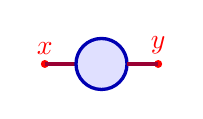
\begin{tikzpicture}[baseline=-0.45ex, scale=0.72]
  \fill[red] (-1,0) circle (2pt) node[above] {$x$};
  \fill[red] (1,0) circle (2pt) node[above] {$y$};
  \draw[purple!80!black, very thick] (-1,0)--(-0.45,0);
  \fill[blue!12, draw=blue!70!black, very thick] (0,0) circle (0.45);
  \draw[purple!80!black, very thick] (0.45,0)--(1,0);
\end{tikzpicture}
\quad=\quad
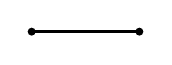
\begin{tikzpicture}[baseline=-0.45ex, scale=0.72]
  \fill ( -0.95,0) circle (2pt);
  \fill ( 0.95,0) circle (2pt);
  \draw[very thick] (-0.95,0)--(0.95,0);
\end{tikzpicture}
\quad+\quad
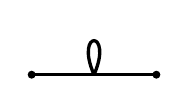
\begin{tikzpicture}[baseline=-0.45ex, scale=0.72]
  \fill (-1.1,0) circle (2pt);
  \fill (1.1,0) circle (2pt);
  \draw[very thick] (-1.1,0)--(1.1,0);
  \draw[very thick] (0,0) .. controls (-0.35,0.8) and (0.35,0.8) .. (0,0);
\end{tikzpicture}
\quad+\quad
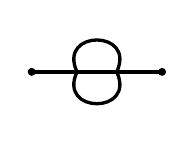
\begin{tikzpicture}[baseline=-0.45ex, scale=0.72]
  \fill (-1.15,0) circle (2pt);
  \fill (1.15,0) circle (2pt);
  \draw[very thick] (-1.15,0)--(1.15,0);
  \draw[very thick] (-0.35,0) .. controls (-0.7,0.75) and (0.7,0.75) .. (0.35,0);
  \draw[very thick] (-0.35,0) .. controls (-0.7,-0.75) and (0.7,-0.75) .. (0.35,0);
\end{tikzpicture}
\quad+\quad
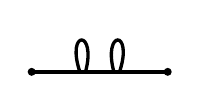
\begin{tikzpicture}[baseline=-0.45ex, scale=0.72]
  \fill (-1.2,0) circle (2pt);
  \fill (1.2,0) circle (2pt);
  \draw[very thick] (-1.2,0)--(1.2,0);
  \draw[very thick] (-0.35,0) .. controls (-0.6,0.75) and (-0.05,0.75) .. (-0.25,0);
  \draw[very thick] (0.35,0) .. controls (0.6,0.75) and (0.05,0.75) .. (0.25,0);
\end{tikzpicture}
\quad+\cdots .
\]
Writing
\[
  G_E(x,y)
  =
  \int\frac{\dd^D k}{(2\pi)^D}
  e^{ik\cdot(x-y)}\widetilde G_E(k),
\]
the Kallen-Lehmann representation says
\[
  G_E(x,y)
  =
  \int_0^\infty\dd\mu^2\,\rho(\mu^2)
  \int\frac{\dd^D k}{(2\pi)^D}
  \frac{e^{ik\cdot(x-y)}}{k^2+\mu^2}.
\]
The self-energy \(\Sigma(k)\) is obtained from one-particle-irreducible
graphs after amputating the external propagators:
\[
  \widetilde G_E(k)
  =
  \frac{1}{k^2+m^2-\Sigma(k)}.
\]
Diagrammatically,
\[
\Sigma(k)
=
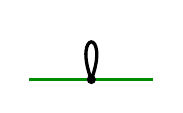
\begin{tikzpicture}[baseline=-0.45ex, scale=0.75]
  \draw[green!55!black, very thick] (-1.05,0)--(1.05,0);
  \fill (0,0) circle (2.2pt);
  \draw[very thick] (0,0) .. controls (-0.32,0.85) and (0.32,0.85) .. (0,0);
\end{tikzpicture}
\quad+\quad
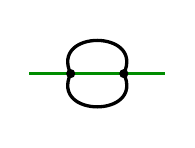
\begin{tikzpicture}[baseline=-0.45ex, scale=0.75]
  \draw[green!55!black, very thick] (-1.15,0)--(1.15,0);
  \fill (-0.45,0) circle (2.2pt);
  \fill (0.45,0) circle (2.2pt);
  \draw[very thick] (-0.45,0) .. controls (-0.8,0.75) and (0.8,0.75) .. (0.45,0);
  \draw[very thick] (-0.45,0) .. controls (-0.8,-0.75) and (0.8,-0.75) .. (0.45,0);
\end{tikzpicture}
\quad+\quad
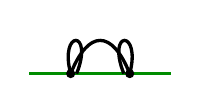
\begin{tikzpicture}[baseline=-0.45ex, scale=0.75]
  \draw[green!55!black, very thick] (-1.2,0)--(1.2,0);
  \fill (-0.5,0) circle (2.2pt);
  \fill (0.5,0) circle (2.2pt);
  \draw[very thick] (-0.5,0) .. controls (-0.7,0.75) and (-0.1,0.75) .. (-0.4,0);
  \draw[very thick] (-0.5,0) .. controls (-0.2,0.75) and (0.2,0.75) .. (0.5,0);
  \draw[very thick] (0.5,0) .. controls (0.7,0.75) and (0.1,0.75) .. (0.4,0);
\end{tikzpicture}
\quad+\cdots .
\]

The Euclidean Feynman rules are as follows. A propagator carrying momentum
\(k\) contributes
\[
\begin{tikzpicture}[baseline=-0.45ex, scale=0.85, >=Stealth]
  \draw[very thick, ->] (-1,0)--(1,0) node[midway, above] {$k$};
\end{tikzpicture}
\qquad =\qquad
\frac{1}{k^2+m^2}.
\]
A vertex contributes
\[
\begin{tikzpicture}[baseline=-0.45ex, scale=0.8, >=Stealth]
  \fill[blue] (0,0) circle (2.5pt);
  \draw[very thick, ->] (-0.85,0.75)--(0,0) node[midway, above left] {$k_1$};
  \draw[very thick, ->] (0.85,0.75)--(0,0) node[midway, above right] {$k_2$};
  \draw[very thick, ->] (0.85,-0.75)--(0,0) node[midway, below right] {$k_3$};
  \draw[very thick, ->] (-0.85,-0.75)--(0,0) node[midway, below left] {$k_4$};
\end{tikzpicture}
\qquad =\qquad
-\frac{g}{4!}\,(2\pi)^D
\delta^D(k_1+k_2+k_3+k_4).
\]
For example, the tadpole contribution is
\[
\begin{tikzpicture}[baseline=-0.45ex, scale=0.75, >=Stealth]
  \draw[green!55!black, very thick, ->] (-1.1,0)--(0,0) node[midway, below] {$k$};
  \draw[green!55!black, very thick, ->] (1.1,0)--(0,0) node[midway, below] {$k$};
  \fill (0,0) circle (2.2pt);
  \draw[very thick, ->] (0,0) .. controls (-0.35,0.9) and (0.35,0.9) .. (0,0)
    node[midway, above] {$k'$};
\end{tikzpicture}
\quad=\quad
4\cdot\frac{3!}{2}
\left(-\frac{g}{4!}\right)
\int\frac{\dd^D k'}{(2\pi)^D}\frac{1}{k'^2+m^2}
\quad=\quad
-\frac{g}{2}
\int\frac{\dd^D k'}{(2\pi)^D}\frac{1}{k'^2+m^2}.
\]
The sunset contribution is
\[
\begin{aligned}
\begin{tikzpicture}[baseline=-0.45ex, scale=0.72, >=Stealth]
  \draw[green!55!black, very thick, ->] (-1.35,0)--(-0.55,0) node[midway, below] {$k$};
  \draw[green!55!black, very thick, ->] (1.35,0)--(0.55,0) node[midway, below] {$k$};
  \fill (-0.55,0) circle (2.2pt);
  \fill (0.55,0) circle (2.2pt);
  \draw[very thick, ->] (-0.55,0) .. controls (-0.8,0.8) and (0.8,0.8) .. (0.55,0)
    node[midway, above] {$k_1$};
  \draw[very thick, ->] (-0.55,0)--(0.55,0) node[midway, above] {$k_2$};
  \draw[very thick, ->] (-0.55,0) .. controls (-0.8,-0.8) and (0.8,-0.8) .. (0.55,0)
    node[midway, below] {$k-k_1-k_2$};
\end{tikzpicture}
&=
4\cdot 4!
\left(-\frac{g}{4!}\right)^2
\int\frac{\dd^D k_1\,\dd^D k_2}{(2\pi)^{2D}}\,
\frac{1}{
  (k_1^2+m^2)(k_2^2+m^2)
  ((k-k_1-k_2)^2+m^2)
}  \\
&=
\frac{g^2}{6}
\int\frac{\dd^D k_1\,\dd^D k_2}{(2\pi)^{2D}}\,
\frac{1}{
  (k_1^2+m^2)(k_2^2+m^2)
  ((k-k_1-k_2)^2+m^2)
}.
\end{aligned}
\]

Let us interpret the order \(g\) contribution to \(\Sigma(k)\),
\[
\begin{tikzpicture}[baseline=-0.45ex, scale=0.75, >=Stealth]
  \draw[green!55!black, very thick, ->] (-1.1,0)--(0,0) node[midway, below] {$k$};
  \draw[green!55!black, very thick, ->] (1.1,0)--(0,0) node[midway, below] {$k$};
  \fill (0,0) circle (2.2pt);
  \draw[very thick, ->] (0,0) .. controls (-0.35,0.9) and (0.35,0.9) .. (0,0)
    node[midway, above] {$k'$};
\end{tikzpicture}
\quad=\quad
-\frac{g}{2}
\int\frac{\dd^D k'}{(2\pi)^D}\frac{1}{k'^2+m^2}.
\]
This is divergent for \(D\ge 2\), but independent of \(k\).
First, regularize the path integral:
\[
  \int[D\phi]
  \longrightarrow
  \int \prod_{|k|\le\Lambda}\dd\widetilde\phi(k).
\]
Then
\[
\begin{aligned}
  -\frac{g}{2}
  \int_{|k'|\le\Lambda}
  \frac{\dd^D k'}{(2\pi)^D}\frac{1}{k'^2+m^2}
  &=
  -\frac{g}{2}
  \frac{\operatorname{vol}(S^{D-1})}{(2\pi)^D}
  \int_0^\Lambda \dd k\,
  \frac{k^{D-1}}{k^2+m^2}  \\
  &\equiv
  -g C_1 .
\end{aligned}
\]
Here
\[
  \operatorname{vol}(S^{D-1})
  =
  \frac{2\pi^{D/2}}{\Gamma(D/2)}
\]
is the area of the unit \((D-1)\)-sphere, and
\[
  \int_0^\Lambda \dd k\,\frac{k^{D-1}}{k^2+m^2}
  =
  \begin{cases}
    \dfrac12\log\dfrac{\Lambda^2+m^2}{m^2}, & D=2,\\[3mm]
    \dfrac{\Lambda^{D-2}}{D-2}+\cdots, & D\ge 3.
  \end{cases}
\]

Recall the Kallen-Lehmann spectral representation:
\[
  \widetilde G_E(k)
  =
  \frac{1}{k^2+m^2-\Sigma(k)}
  =
  \frac{Z}{k^2+m_*^2}
  +
  \int_{\mu^2\ge 4m_*^2}\dd\mu^2\,
  \frac{\sigma(\mu^2)}{k^2+\mu^2}.
\]
The parameter \(m_*\) is the actual mass of the particle, corresponding to
the pole in \(k^2\), or just \(k^D\) at fixed
\(\vec k=(k^1,\ldots,k^{D-1})\), closest to the origin. A constant term at
order \(g\) in \(\Sigma(k)\) shifts the pole position:
\[
  m_*^2=m^2+gC_1+O(g^2),
\]
where
\[
  C_1\sim
  \begin{cases}
    \log\Lambda, & D=2,\\
    \Lambda^{D-2}, & D\ge 3.
  \end{cases}
\]

The interpretation is as follows.
\begin{enumerate}[label=\arabic*.]
  \item \(m_*\) is the mass of the particle.
  \item \(m\) is just some parameter in the Lagrangian; its relation to the
  physical mass is dependent on the regularization scheme.
  \item It is standard terminology to refer to \(m\) as the bare mass, and to
  the Lagrangian that enters the regularized path integral as the bare
  Lagrangian.
  \item One might be slightly disturbed by the fact that while the difference
  between \(m^2\) and \(m_*^2\) is formally suppressed by the coupling \(g\),
  the coefficient \(C_1\) diverges as \(\Lambda\to\infty\), and so \(gC_1\)
  is not exactly small.
\end{enumerate}

One way to handle this in a consistent manner in perturbation theory is to
write
\[
  m^2=m_R^2+\delta m^2,
\]
where \(m_R\) is a finite renormalized mass close to \(m_*\), and
\(\delta m^2\) is viewed as a counterterm, diverging as
\(\Lambda\to\infty\), but appearing at order \(g\). Generally,
\[
  \delta m^2=\sum_{n=1}^{\infty}(\delta m^2)^{(n)}g^n .
\]
The coefficient \((\delta m^2)^{(n)}\) is chosen to cancel the divergent
contribution to the pole position \(m_*^2\) at order \(g^n\) in perturbation
theory. For example,
\[
  m_*^2=m_R^2+\delta m^2+gC_1+O(g^2),
\]
so we choose
\[
  (\delta m^2)^{(1)}=-C_1+\text{finite}.
\]
Correspondingly, we split the bare Lagrangian as
\[
  \mathcal L^E
  =
  \mathcal L_R^E+\Delta\mathcal L^E,
  \qquad
  \Delta\mathcal L^E=\frac12\delta m^2\phi^2,
\]
where \(\mathcal L_R^E\) contains the term \(\frac12m_R^2\phi^2\). We then
treat \(\Delta\mathcal L^E\) as producing interaction vertices at order
\(g^n\):
\[

\begin{tikzpicture}[baseline=-0.45ex, scale=0.85]
  \draw[purple!80!black, very thick] (-1,0)--(1,0);
  \fill (0,0) circle (2.4pt);
\end{tikzpicture}
\qquad\longleftrightarrow\qquad
-(\delta m^2)^{(n)}g^n\phi^2 .
\]
The separation of \(m^2\) into \(m_R^2\) and \(\delta m^2\) is entirely ad hoc.
Its only purpose is to reorganize perturbation theory so that when we take
\(\Lambda\to\infty\), divergences cancel manifestly at each order in \(g\), as
opposed to cancelling divergences between different orders in \(g\), for
example between \(m^2\) at zeroth order and \(C_1g\) at first order.

To make meaningful physical predictions, we should pick a regularization
scheme, find the relation between \(m\) and \(m_*\), compute observables using
the Lagrangian that includes \(m^2=m_R^2+\delta m^2\), and express the result
in terms of \(m_*\), the physical mass.

For a four-point function,
\[
  \langle
    \phi(x_1^E)\phi(x_2^E)\phi(x_3^E)\phi(x_4^E)
  \rangle,
\]
the disconnected and connected pieces are
\[
\begin{aligned}
  &\langle
    \phi(x_1^E)\phi(x_2^E)\phi(x_3^E)\phi(x_4^E)
  \rangle  \\
  &\quad =
  \langle\phi(x_1^E)\phi(x_2^E)\rangle
  \langle\phi(x_3^E)\phi(x_4^E)\rangle
  +(2\leftrightarrow 4)
  +(2\leftrightarrow 3)  \\
  &\qquad
  +
  \langle
    \phi(x_1^E)\phi(x_2^E)\phi(x_3^E)\phi(x_4^E)
  \rangle_{\mathrm{conn}} .
\end{aligned}
\]

\begin{center}
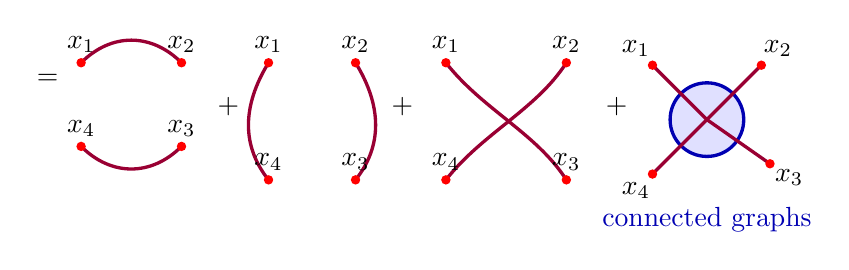
\begin{tikzpicture}[scale=0.85]
  \node at (-0.5,1.65) {$=$};
  \draw[purple!80!black, very thick] (0,1.9) .. controls (0.45,2.35) and (1.05,2.35) .. (1.5,1.9);
  \draw[purple!80!black, very thick] (0,0.65) .. controls (0.45,0.2) and (1.05,0.2) .. (1.5,0.65);
  \foreach \p/\lab in {(0,1.9)/x_1,(1.5,1.9)/x_2,(1.5,0.65)/x_3,(0,0.65)/x_4} {
    \fill[red] \p circle (2pt);
    \node[above] at \p {$\lab$};
  }

  \node at (2.2,1.25) {$+$};
  \draw[purple!80!black, very thick] (2.8,1.9) .. controls (2.4,1.25) and (2.4,0.65) .. (2.8,0.15);
  \draw[purple!80!black, very thick] (4.1,1.9) .. controls (4.5,1.25) and (4.5,0.65) .. (4.1,0.15);
  \foreach \p/\lab in {(2.8,1.9)/x_1,(4.1,1.9)/x_2,(4.1,0.15)/x_3,(2.8,0.15)/x_4} {
    \fill[red] \p circle (2pt);
    \node[above] at \p {$\lab$};
  }

  \node at (4.8,1.25) {$+$};
  \draw[purple!80!black, very thick] (5.45,1.9) .. controls (6.0,1.2) and (6.8,0.85) .. (7.25,0.15);
  \draw[purple!80!black, very thick] (7.25,1.9) .. controls (6.8,1.2) and (6.0,0.85) .. (5.45,0.15);
  \foreach \p/\lab in {(5.45,1.9)/x_1,(7.25,1.9)/x_2,(7.25,0.15)/x_3,(5.45,0.15)/x_4} {
    \fill[red] \p circle (2pt);
    \node[above] at \p {$\lab$};
  }

  \node at (8.0,1.25) {$+$};
  \fill[blue!12, draw=blue!70!black, very thick] (9.35,1.05) circle (0.55);
  \foreach \ang/\lab in {135/x_1,45/x_2,-35/x_3,-135/x_4} {
    \draw[purple!80!black, very thick]
      (9.35,1.05) -- ({9.35+1.15*cos(\ang)},{1.05+1.15*sin(\ang)});
    \fill[red] ({9.35+1.15*cos(\ang)},{1.05+1.15*sin(\ang)}) circle (2pt);
    \node at ({9.35+1.5*cos(\ang)},{1.05+1.5*sin(\ang)}) {$\lab$};
  }
  \node[blue!70!black] at (9.35,-0.45) {connected graphs};
\end{tikzpicture}
\end{center}

The final term is the connected correlator.

Define its Fourier transform by
\[
\begin{aligned}
  G_E^{\mathrm{conn}}(x_1^E,\ldots,x_4^E)
  &=
  \left\langle
    \phi(x_1^E)\cdots\phi(x_4^E)
  \right\rangle_{\mathrm{conn}}  \\
  &\equiv
  \int
  \frac{\dd^Dk_1^E}{(2\pi)^D}\cdots
  \frac{\dd^Dk_4^E}{(2\pi)^D}\,
  \ee^{\ii k_1^E\cdot x_1^E+\cdots+\ii k_4^E\cdot x_4^E}
  \widetilde G_E^{\mathrm{conn}}(k_1^E,\ldots,k_4^E).
\end{aligned}
\]
To leading order in \(g\),
\[
\begin{aligned}
  \widetilde G_E^{\mathrm{conn}}(k_1^E,\ldots,k_4^E)
  &=
  \begin{tikzpicture}[baseline=-0.6ex, scale=0.8, >=Stealth]
    \fill[blue!80!black] (0,0) circle (3pt);
    \foreach \ang/\lab in {140/k_1,40/k_2,-40/k_3,-140/k_4} {
      \draw[purple!80!black, very thick, ->]
        ({1.1*cos(\ang)},{1.1*sin(\ang)}) -- (0,0);
      \fill[red] ({1.1*cos(\ang)},{1.1*sin(\ang)}) circle (1.8pt);
      \node[blue!70!black] at ({1.45*cos(\ang)},{1.45*sin(\ang)}) {$\lab$};
    }
  \end{tikzpicture}
  +\cdots  \\
  &=
  (2\pi)^D
  \delta^D(k_1^E+k_2^E+k_3^E+k_4^E)
  \left[
    -g
    \prod_{j=1}^{4}
    \frac{1}{(k_j^E)^2+m^2}
    +O(g^2)
  \right].
\end{aligned}
\]
As above, one can write
\[
  m^2=m_R^2+\delta m^2
\]
and expand in \(\delta m^2\), regrouping the terms according to powers of
\(g\). A convenient choice is \(m_R=m_*\).

\subsection{Lorentzian Green Functions}

Everything said so far about the perturbative computation of
\[
  G_E(x_1^E,\ldots,x_n^E)
\]
can be equally applied to computing the time-ordered Green function
\[
  G(x_1,\ldots,x_n)
  =
  \langle\Omega|
  T\hat\phi(x_1)\cdots\hat\phi(x_n)
  |\Omega\rangle,
\]
with the modification of Feynman rules:
\[
\begin{array}{ccl}
\begin{tikzpicture}[baseline=-0.5ex, scale=0.85, >=Stealth]
  \draw[purple!80!black, very thick, ->] (-1,0)--(1,0);
  \node[blue!70!black, above] at (0,0.05) {$k$};
\end{tikzpicture}
&=&
\displaystyle
\frac{-\ii}{k^2+m^2-\ii\epsilon},
\\[2.0em]
\begin{tikzpicture}[baseline=-0.6ex, scale=0.72, >=Stealth]
  \fill[blue!80!black] (0,0) circle (3pt);
  \foreach \ang/\lab in {140/k_1,40/k_2,-40/k_3,-140/k_4} {
    \draw[purple!80!black, very thick, ->]
      ({1.0*cos(\ang)},{1.0*sin(\ang)}) -- (0,0);
    \node[blue!70!black] at ({1.3*cos(\ang)},{1.3*sin(\ang)}) {$\lab$};
  }
\end{tikzpicture}
&=&
\displaystyle
-\frac{\ii g}{4!}\,
(2\pi)^D\delta^D(k_1+k_2+k_3+k_4).
\end{array}
\]
All momenta \(k^\mu\) are now Lorentzian, for example
\[
  k^2\equiv \eta_{\mu\nu}k^\mu k^\nu.
\]
For instance, the one-loop tadpole is
\[
\begin{tikzpicture}[baseline=-0.5ex, scale=0.75, >=Stealth]
  \draw[purple!80!black, very thick, ->] (-1.3,0)--(-0.05,0);
  \draw[purple!80!black, very thick, ->] (0.05,0)--(1.3,0);
  \draw[purple!80!black, very thick]
    (0,0) .. controls (-0.42,0.88) and (0.42,0.88) .. (0,0);
  \fill (0,0) circle (2.2pt);
  \node[blue!70!black] at (-1.0,-0.33) {$k$};
  \node[blue!70!black] at (1.0,-0.33) {$k$};
  \node[blue!70!black] at (0,0.92) {$k'$};
\end{tikzpicture}
=
-\frac{\ii g}{2}
\int\frac{\dd^Dk'}{(2\pi)^D}
\frac{-\ii}{k'^2+m^2-\ii\epsilon}.
\]
In the complex \((k')^0\)-plane this may be Wick rotated:
\begin{center}
\begin{tikzpicture}[baseline=-0.5ex, scale=0.95, >=Stealth]
  \draw[line width=0.55pt] (-2.65,-1.7) rectangle (2.65,1.7);
  \draw[->,green!50!black, thick] (-2.35,0)--(2.35,0) node[right] {$\mathbb R$};
  \draw[->,purple!80!black, thick] (0,-1.45)--(0,1.45);
  \node[purple!80!black, above] at (0,1.45) {cplx \((k')^0\)};
  \node[red] at (-1.35,0.32) {\(\times\)};
  \node[red] at (1.35,-0.32) {\(\times\)};
  \draw[->,orange!85!black, very thick]
    (1.05,1.08) .. controls (0.5,0.92) and (0.32,0.45) .. (-0.16,0.42);
  \draw[->,orange!85!black, very thick]
    (-1.05,-1.05) .. controls (-0.55,-0.9) and (-0.35,-0.45) .. (0.18,-0.42);
  \node[orange!85!black] at (1.25,1.05) {Wick rotation};
  \node[purple!80!black, right] at (2.55,1.15) {\((k')^0=\ii k^D\)};
\end{tikzpicture}
\end{center}
The rotation gives
\[
\begin{aligned}
-\frac{\ii g}{2}
\int\frac{\dd^Dk'}{(2\pi)^D}
\frac{-\ii}{k'^2+m^2-\ii\epsilon}
=
\ii\left[
-\frac{g}{2}
\int\frac{\dd^Dk_E'}{(2\pi)^D}
\frac{1}{(k_E')^2+m^2}
\right].
\end{aligned}
\]
Thus this contribution is to \(\ii\Sigma(k)\), consistently with the
Euclidean computation.

The full time-ordered two-point function takes the form
\[
  G(x,y)
  =
  \int\frac{\dd^Dk}{(2\pi)^D}
  \ee^{\ii k\cdot(x-y)}
  \widetilde G(k),
\]
where
\[
  \widetilde G(k)
  =
  \frac{-\ii}{k^2+m^2-\ii\epsilon-\Sigma(k)}.
\]
The function \(\Sigma(k)\) is expected to have a pair of branch cuts in
\(k^0\), starting at the multi-particle threshold
\[
  -k^2=M^2,
\]
where \(M\) is the invariant mass of the lightest multi-particle state.
These branch cuts may be chosen to extend along the real \(k^0\)-axis:
\[
  k^0>\sqrt{\vec k^2+M^2},
  \qquad
  k^0<-\sqrt{\vec k^2+M^2}.
\]

\begin{center}
\begin{tikzpicture}[scale=0.95, >=Stealth]
  \draw[line width=0.55pt] (-3.0,-2.0) rectangle (3.0,2.0);
  \draw[->,blue!70!black, thick] (-2.65,0)--(2.65,0)
    node[right] {$\operatorname{Re} k^0$};
  \draw[->,green!50!black, thick] (0,-1.75)--(0,1.75)
    node[above] {$\operatorname{Im} k^0$};
  \draw[red!80!black, very thick, decorate,
    decoration={zigzag,segment length=4pt,amplitude=1.2pt}]
    (-2.65,0)--(-1.0,0);
  \draw[red!80!black, very thick, decorate,
    decoration={zigzag,segment length=4pt,amplitude=1.2pt}]
    (1.0,0)--(2.65,0);
  \node[below] at (-1.0,-0.05)
    {$-\sqrt{\vec k^2+M^2}$};
  \node[below] at (1.0,-0.05)
    {$\sqrt{\vec k^2+M^2}$};
  \draw[->,orange!85!black, very thick]
    (1.55,1.0) .. controls (2.1,0.8) and (2.1,0.3) .. (1.55,0.12);
  \draw[->,orange!85!black, very thick]
    (-1.45,-1.0) .. controls (-2.05,-0.8) and (-2.05,-0.3) .. (-1.45,-0.12);
  \node[blue!70!black, anchor=west] at (-2.75,1.65) {cplx \(k^0\)};
\end{tikzpicture}
\end{center}

The actual value of \(\Sigma(k)\) at real \(k^0\) is determined by our Wick
rotation procedure relating \(G_E\) to \(G\). For example, for real
\[
  k^0>\sqrt{\vec k^2+M^2},
\]
\(\Sigma(k)\) is given by analytic continuation from \(k^0\in\ii\mathbb R\)
(or, more generally, complex \(k^0\) on the ``first sheet'') to the positive
real \(k^0\)-axis from above.

\section{Scattering Theory}

We now introduce in- and out-basis states.

\begin{center}
\begin{tikzpicture}[scale=0.95, >=Stealth]
  \draw[->, thick] (-3.3,-2.4)--(-3.3,2.5) node[above] {$t$};
  \draw[->, thick] (-3.3,-2.4)--(-1.1,-2.4) node[right] {$\vec x$};
  \fill[pattern=north east lines, pattern color=black!55, draw=black,
    line width=0.9pt] (0,0) ellipse (1.2 and 0.55);
  \draw[blue!75!black, dashed, thick] (-1.9,1.45)--(2.2,1.45);
  \draw[green!50!black, dashed, thick] (-1.9,-1.45)--(2.2,-1.45);
  \foreach \x in {-0.55,0.15,0.85} {
    \draw[->, blue!75!black, very thick]
      (\x,0.45)--({\x+0.55},1.55);
  }
  \foreach \x in {-0.55,0.55} {
    \draw[->, green!50!black, very thick]
      ({\x-0.55},-1.55)--(\x,-0.45);
  }
  \node[blue!75!black, align=left, anchor=west] at (2.45,1.45)
    {out-basis: states that look like far-separated\\
     (wave packets of) particles in the far future};
  \node[green!50!black, align=left, anchor=west] at (2.45,-1.45)
    {in-basis: states that look like far-separated\\
     particles in the far past};
\end{tikzpicture}
\end{center}

One can label out- or in-basis states as if they consist of free particles:
\[
  |\vec k_1,\vec k_2,\ldots,\vec k_n\rangle^{\mathrm{out}},
  \qquad
  |\vec k_1,\vec k_2,\ldots,\vec k_n\rangle^{\mathrm{in}}.
\]
For now we assume one particle species. Otherwise one also adds labels of
particle type and helicity, and so on.

Either the out-basis states \(|\alpha\rangle^{\mathrm{out}}\) or the in-basis
states \(|\alpha\rangle^{\mathrm{in}}\) span the entire Hilbert space
\(\mathcal H\). In an interacting QFT, the in- and out-bases are different,
and are related by a linear change of basis:
\[
  {}^{\mathrm{out}}\langle\beta|\alpha\rangle^{\mathrm{in}}
  \equiv S_{\beta\alpha},
\]
the \(S\)-matrix. Equivalently,
\[
  |\alpha\rangle^{\mathrm{in}}
  =
  \int\dd\beta\,
  S_{\beta\alpha}|\beta\rangle^{\mathrm{out}},
\]
with normalization
\[
  \int\dd\beta\,
  S_{\gamma\beta}^{\dagger}S_{\beta\alpha}
  =
  \delta_{\gamma\alpha}.
\]
Next we will give an explicit construction of in- or out-basis states using
the local field operator \(\hat\phi(x)\), thereby relating the \(S\)-matrix to
correlators of \(\hat\phi\). This is the Haag-Ruelle construction.

\subsection{Smeared Operators and One-Particle States}

Recall that
\[
\begin{aligned}
  \hat\phi(x)|\Omega\rangle
  &=
  \int\dd^{D-1}\vec k\,
  \ee^{-\ii\vec k\cdot\vec x+\ii\omega_{\vec k}x^0}
  \left[
    \frac{Z}{(2\pi)^{D-1}2\omega_{\vec k}}
  \right]^{1/2}
  |\vec k\rangle  \\
  &\quad
  +
  \int\dd\alpha\,
  \ee^{-\ii P_\alpha\cdot x}
  \langle\alpha|\hat\phi(0)|\Omega\rangle
  |\alpha\rangle .
\end{aligned}
\]
The second term is the multi-particle part. The multi-particle states are
separated from the one-particle states by a gap in their invariant masses.

Consider a smearing function \(f(x)\), \(x\in\mathbb R^{1,D-1}\), with
\[
  f(x)
  =
  \int\frac{\dd^Dk}{(2\pi)^D}\,\widetilde f(k)\,
  \ee^{\ii k\cdot x},
\]
such that \(\widetilde f(k)\) is supported near the mass shell
\[
  k^0>0,\qquad k^2+m^2=0,
\]
and at the same time \(f(x)\) is concentrated in a finite domain in spacetime.
For example, take the Gaussian profile
\[
\begin{aligned}
  f(x)
  &=
  \frac{1}{(2\pi)^{D/2}L^D}
  \exp\biggl[
    -\frac{1}{2L^2}(x^0-t_*)^2
    -\frac{1}{2L^2}(\vec x-\vec x_*)^2  \\
  &\hspace{3.7cm}
    +\ii\vec P_*\cdot(\vec x-\vec x_*)
    -\ii E_*(x^0-t_*)
  \biggr],
\end{aligned}
\]
for some large constant distance \(L>0\). Then
\[
  \widetilde f(k)
  =
  \exp\left[
    -\frac{L^2}{2}(k^0-E_*)^2
    -\frac{L^2}{2}(\vec k-\vec P_*)^2
    -\ii\vec k\cdot\vec x_*
    +\ii k^0t_*
  \right],
\]
peaked near
\[
  (k^0,\vec k)\simeq(E_*,\vec P_*),
\]
but still remembering \((t_*,\vec x_*)\).

A more convenient choice is to make \(\widetilde f(k)\) compactly supported
within a momentum domain of size \(\sim 1/L\), but still smooth. In that case
\(f(x)\) spreads to a blob of size \(\sim L\) and diminishes outside the blob
faster than \(|x|^{-N}\) for any \(N>0\) as \(|x|\to\infty\).

We further choose \((E_*,\vec P_*)\) such that
\[
  E_*^2-\vec P_*^{\,2}=m^2.
\]
Now consider the smeared operator
\[
  \hat\phi_f
  \equiv
  \int\dd^Dx\, f(x)\hat\phi(x).
\]
Then
\[
\begin{aligned}
  \hat\phi_f|\Omega\rangle
  &=
  \int\dd^{D-1}\vec k\,
  \widetilde f(\omega_{\vec k},\vec k)
  \left[
    \frac{Z}{(2\pi)^{D-1}2\omega_{\vec k}}
  \right]^{1/2}
  |\vec k\rangle \\
  &\quad
  +
  \int_{\mathrm{m.p.}}\dd\alpha\,
  \widetilde f(P_\alpha)
  \langle\alpha|\hat\phi(0)|\Omega\rangle
  |\alpha\rangle .
\end{aligned}
\]
The multi-particle contribution is suppressed by our choice of
\(\widetilde f(k)\), so only the one-particle state is retained.

Define the transformation \(f(x)\mapsto f^{(T)}(x)\) by setting
\[
  \widetilde f^{(T)}(k)
  :=
  \ee^{\ii(k^0-\omega_{\vec k})T}\widetilde f(k),
  \qquad
  \omega_{\vec k}=\sqrt{\vec k^2+m^2}.
\]
In particular,
\[
  \widetilde f^{(T)}(\omega_{\vec k},\vec k)
  =
  \widetilde f(\omega_{\vec k},\vec k),
\]
independent of \(T\). Therefore the one-particle part of
\(\hat\phi_{f^{(T)}}|\Omega\rangle\) is independent of \(T\). With the above
prescribed \(f(x)\), the multi-particle component of
\(\hat\phi_{f^{(T)}}|\Omega\rangle\) is negligible, and therefore
\[
  \hat\phi_{f^{(T)}}|\Omega\rangle
  \simeq
  \hat\phi_f|\Omega\rangle.
\]
The approximation is uniformly valid for all \(T\), including arbitrarily
large \(T\).

What does \(f^{(T)}(x)\) look like? By definition,
\[
  f^{(T)}(x)
  =
  \int\frac{\dd^Dk}{(2\pi)^D}\,
  \ee^{\ii k\cdot x+\ii(k^0-\omega_{\vec k})T}
  \widetilde f(k).
\]
Equivalently,
\[
\begin{aligned}
  f^{(T)}(x)
  &=
  \int\dd^Dy\,
  \int\frac{\dd^Dk}{(2\pi)^D}\,
  \ee^{\ii k\cdot(x-y)+\ii(k^0-\omega_{\vec k})T}
  f(y) \\
  &=
  \int\dd^Dy\,
  \delta(x^0-y^0-T)
  \int\frac{\dd^{D-1}\vec k}{(2\pi)^{D-1}}\,
  \ee^{\ii\vec k\cdot(\vec x-\vec y)-\ii\omega_{\vec k}T}
  f(y) \\
  &=
  \int\dd^{D-1}\vec y\,
  K(\vec x-\vec y;T)\,
  f(x^0-T,\vec y),
\end{aligned}
\]
where
\[
  K(\vec x;T)
  =
  \int\frac{\dd^{D-1}\vec k}{(2\pi)^{D-1}}\,
  \ee^{\ii\vec k\cdot\vec x-\ii\omega_{\vec k}T}.
\]
The kernel \(K(\vec x;T)\) obeys the Klein-Gordon equation
\[
  \left(
    \frac{\partial^2}{\partial\vec x^{\,2}}
    -
    \frac{\partial^2}{\partial T^2}
    -
    m^2
  \right)
  K(\vec x;T)=0,
\]
with initial condition
\[
  K(\vec x;0)=\delta^{D-1}(\vec x).
\]
If \(\widetilde f(k)\) is peaked at
\[
  k_*\simeq(E_*,\vec P_*),
\]
then \(f^{(T)}(x^0,\vec x)\) looks like the wave packet
\[
  f(x^0-T,\vec x)
\]
having moved with group velocity
\[
  \vec v
  =
  \frac{\partial\omega_{\vec P_*}}{\partial\vec P_*}
  =
  \frac{\vec P_*}{E_*}
\]
for time \(T\).

\begin{center}
\begin{tikzpicture}[scale=0.95, >=Stealth]
  \draw[->, thick] (-2.7,-1.65)--(-2.7,2.6) node[above] {$x^0$};
  \draw[->, thick] (-2.7,-1.65)--(3.2,-1.65) node[right] {$\vec x$};
  \fill[blue!8, draw=blue!80!black, very thick]
    (-0.7,-0.75) ellipse (0.95 and 0.55);
  \foreach \s in {-0.35,0,0.35} {
    \draw[blue!80!black, thick] (-1.2+\s,-1.0)--(-0.55+\s,-0.45);
  }
  \fill[purple!8, draw=purple!80!black, very thick]
    (1.45,1.35) ellipse (0.95 and 0.55);
  \foreach \s in {-0.35,0,0.35} {
    \draw[purple!80!black, thick] (0.95+\s,1.1)--(1.6+\s,1.65);
  }
  \draw[->, green!60!black, very thick] (-0.1,-0.25)--(1.15,0.95);
  \node[blue!80!black] at (0.35,-0.7) {$\operatorname{supp}(f)$};
  \node[purple!80!black] at (2.65,1.7)
    {$\operatorname{supp}(f^{(T)})$};
  \node[green!60!black] at (0.95,0.22) {$\Delta\vec x=\vec vT$};
  \draw[dashed, gray] (-1.75,-0.75)--(2.45,-0.75);
  \draw[dashed, gray] (0.1,1.35)--(2.45,1.35);
\end{tikzpicture}
\end{center}

Evolving \(f\mapsto f^{(T)}\), the support of \(f(x)\), say a region in
spacetime of large size \(\sim L\) centered around \((t_*,\vec x_*)\), moves
to a region centered around
\[
  (t_*+T,\vec x_*+\vec vT),
\]
and yet
\[
  \hat\phi_{f^{(T)}}|\Omega\rangle
  \simeq
  \hat\phi_f|\Omega\rangle.
\]
It is the same one-particle state. This may seem counterintuitive, but there
is no contradiction: there are a lot more operators than states.

Now consider a pair of functions \(f_1(x)\), \(f_2(x)\) of the above prescribed
form, whose Fourier transforms \(\widetilde f_1(k)\), \(\widetilde f_2(k)\)
are supported near \(k\simeq k_1,k_2\) respectively,
\[
  k_1^2=k_2^2=-m^2.
\]
Also assume
\[
  \vec k_1\neq \vec k_2 .
\]

\begin{center}
\begin{tikzpicture}[>=Stealth,scale=0.95]
  \begin{scope}[shift={(-3.7,0)}]
    \draw[->, thick] (0,-2.1)--(0,2.1) node[above] {$p^0$};
    \draw[->, thick] (0,-2.1)--(2.6,-3.0) node[below] {$p^1$};
    \draw[->, thick] (0,-2.1)--(3.0,-1.75) node[right] {$p^2$};
    \draw[blue!75!black, very thick]
      (-2.1,0.35) .. controls (-1.45,1.9) and (1.45,1.9) .. (2.1,0.35);
    \draw[blue!75!black, very thick]
      (-2.1,0.35) .. controls (-1.15,-0.15) and (1.15,-0.15) .. (2.1,0.35);
    \fill[purple!25,draw=purple!80!black,very thick]
      (-0.85,0.35) ellipse (0.32 and 0.22);
    \foreach \s in {-0.12,0.08}
      \draw[purple!80!black,thick] (-1.05+\s,0.23)--(-0.72+\s,0.48);
    \fill[green!25,draw=green!55!black,very thick]
      (1.05,0.55) ellipse (0.32 and 0.22);
    \foreach \s in {-0.12,0.08}
      \draw[green!55!black,thick] (0.85+\s,0.43)--(1.18+\s,0.68);
    \node[purple!80!black] at (-1.25,-0.2) {$k_1$};
    \node[green!55!black] at (1.75,0.57) {$\sim k_2$};
  \end{scope}

  \begin{scope}[shift={(3.4,-0.4)}]
    \draw[->, thick] (-2.2,-1.5)--(-2.2,2.1) node[above] {$x^0$};
    \draw[->, thick] (-2.2,-1.5)--(2.9,-1.5) node[right] {$\vec x$};
    \fill[blue!12,draw=blue!75!black,very thick]
      (-0.25,-1.3) ellipse (0.62 and 0.38);
    \fill[green!12,draw=green!55!black,very thick]
      (0.35,-1.3) ellipse (0.62 and 0.38);
    \fill[blue!12,draw=blue!75!black,very thick]
      (-0.75,0.75) ellipse (0.55 and 0.35);
    \fill[green!12,draw=green!55!black,very thick]
      (1.4,0.55) ellipse (0.55 and 0.35);
    \foreach \x/\c in {-0.25/blue!75!black,0.35/green!55!black,
                       -0.75/blue!75!black,1.4/green!55!black} {
      \draw[\c,thick] (\x-0.22,-1.42)--(\x+0.12,-1.18);
    }
    \draw[->,blue!75!black,thick] (-0.35,-0.95)--(-0.68,0.38);
    \draw[->,green!55!black,thick] (0.48,-0.95)--(1.18,0.25);
    \node[blue!75!black] at (-1.55,0.95) {$f_1^{(T)}$};
    \node[green!55!black] at (2.15,0.82) {$f_2^{(T)}$};
  \end{scope}
\end{tikzpicture}
\end{center}

The regions of concentration of \(f_1^{(T)}\) and \(f_2^{(T)}\) move apart as
\[
  T\to\pm\infty,
\]
and become far space-like separated.

\subsection{Multi-Particle In/Out States}

Consider the state
\[
  |\Psi^{(T)}\rangle
  \equiv
  \hat\phi_{f_1^{(T)}}\hat\phi_{f_2^{(T)}}|\Omega\rangle .
\]
The overlap between \(|\Psi^{(T)}\rangle\) and \(|\Psi^{(T')}\rangle\) is
\[
\begin{aligned}
  \langle\Psi^{(T)}|\Psi^{(T')}\rangle
  &=
  \langle\Omega|
  \hat\phi_{f_2^{(T)}*}
  \hat\phi_{f_1^{(T)}*}
  \hat\phi_{f_1^{(T')}}
  \hat\phi_{f_2^{(T')}}
  |\Omega\rangle .
\end{aligned}
\]
Fix
\[
  T'-T\equiv\Delta T,
  \qquad
  \text{send }T\to\pm\infty .
\]

\begin{center}
\begin{tikzpicture}[>=Stealth,scale=0.95]
  \draw[->,thick] (-3.3,-1.8)--(-3.3,2.0) node[above] {$x^0$};
  \draw[->,thick] (-3.3,-1.8)--(3.4,-1.8) node[right] {$\vec x$};
  \fill[purple!15,draw=purple!85!black,very thick] (-2.1,-1.1) ellipse (0.45 and 0.3);
  \fill[blue!12,draw=blue!75!black,very thick] (-1.45,0.65) ellipse (0.48 and 0.3);
  \fill[green!12,draw=green!55!black,very thick] (2.0,-1.0) ellipse (0.45 and 0.3);
  \fill[teal!12,draw=teal!70!black,very thick] (2.55,0.55) ellipse (0.48 and 0.3);
  \draw[<->,purple!80!black,very thick] (-0.8,0.15)--(1.2,0.0)
    node[midway,above,align=center] {large spacelike\\separation};
  \node[purple!85!black] at (-2.7,-0.72) {$f_1^{(T')}$};
  \node[blue!75!black] at (-2.0,1.08) {$f_1^{(T)}$};
  \node[green!55!black] at (2.6,-0.65) {$f_2^{(T')}$};
  \node[teal!70!black] at (3.1,0.95) {$f_2^{(T)}$};
\end{tikzpicture}
\end{center}

By the cluster property,
\[
\begin{aligned}
&\langle\Omega|
  \hat\phi_{f_2^{(T)}*}
  \hat\phi_{f_1^{(T)}*}
  \hat\phi_{f_1^{(T')}}
  \hat\phi_{f_2^{(T')}}
  |\Omega\rangle
\\
&\qquad\longrightarrow
  \langle\Omega|
  \hat\phi_{f_1^{(T)}*}
  \hat\phi_{f_1^{(T')}}
  |\Omega\rangle\,
  \langle\Omega|
  \hat\phi_{f_2^{(T)}*}
  \hat\phi_{f_2^{(T')}}
  |\Omega\rangle ,
\end{aligned}
\]
which is independent of \(\Delta T\). It follows that
\[
  \bigl\|\,|\Psi^{(T')}\rangle-|\Psi^{(T)}\rangle\,\bigr\|
  \longrightarrow 0
  \qquad
  \text{as }T\to\pm\infty .
\]
In fact, with non-overlapping and smooth \(\widetilde f_i(k)\), this norm
vanishes faster than \(|T|^{-N}\) for any \(N>0\) as \(T\to\pm\infty\)
\((\text{Hepp }1965)\).

Thus
\[
  \lim_{T\to\pm\infty}
  \hat\phi_{f_1^{(T)}}\hat\phi_{f_2^{(T)}}|\Omega\rangle
  :=
  |\phi_{f_1},\phi_{f_2}\rangle^{\mathrm{out/in}}
\]
is a well-defined state in \(\mathcal H\). Compare this with
\[
  \hat\phi_f|\Omega\rangle
  =
  \int\dd^{D-1}\vec k\,
  \widetilde f(\omega_{\vec k},\vec k)
  \left[
    \frac{Z}{(2\pi)^{D-1}2\omega_{\vec k}}
  \right]^{1/2}
  |\vec k\rangle ,
\]
assuming \(\operatorname{supp}\widetilde f\) is concentrated near the
one-particle mass shell, with no overlap with the multi-particle momentum
region. We can write
\[
\begin{aligned}
  |\phi_{f_1},\phi_{f_2}\rangle^{\mathrm{out/in}}
  &=
  \int\prod_{j=1}^2 \dd^{D-1}\vec k_j\,
  \widetilde f_j(\omega_{\vec k_j},\vec k_j)
  \left[
    \frac{Z}{(2\pi)^{D-1}2\omega_{\vec k_j}}
  \right]^{1/2}
  |\vec k_1,\vec k_2\rangle^{\mathrm{out/in}} .
\end{aligned}
\]

Using the cluster property, one can verify that
\(|\vec k_1,\vec k_2\rangle^{\mathrm{out/in}}\) obey the orthogonality
\[
\begin{aligned}
  {}^{\mathrm{out}}\langle
  \vec k_1,\vec k_2|\vec k_1',\vec k_2'
  \rangle^{\mathrm{out}}
  &=
  \delta^{D-1}(\vec k_1-\vec k_1')\,
  \delta^{D-1}(\vec k_2-\vec k_2')
  +(\vec k_1'\leftrightarrow\vec k_2'),
\end{aligned}
\]
and the same with
\[
  {}^{\mathrm{in}}\langle
  \vec k_1,\vec k_2|\vec k_1',\vec k_2'
  \rangle^{\mathrm{in}} .
\]

The generalization to \(n\)-particle in/out-states
\[
  |\vec k_1,\ldots,\vec k_n\rangle^{\mathrm{in/out}}
\]
is obvious. Given \(f_1(x),\ldots,f_n(x)\) whose Fourier transforms
\(\widetilde f_1(k),\ldots,\widetilde f_n(k)\) are supported near the mass
shell
\[
  k^2+m^2=0,
  \qquad
  k^0>0,
\]
and do not overlap,
\[
\begin{aligned}
  \lim_{T\to\pm\infty}
  \hat\phi_{f_1^{(T)}}\cdots\hat\phi_{f_n^{(T)}}|\Omega\rangle
  &:=
  |\phi_{f_1},\ldots,\phi_{f_n}\rangle^{\mathrm{out/in}} \\
  &=
  \int\prod_{j=1}^n \dd^{D-1}\vec k_j\,
  \widetilde f_j(\omega_{\vec k_j},\vec k_j)
  \left[
    \frac{Z}{(2\pi)^{D-1}2\omega_{\vec k_j}}
  \right]^{1/2}
  |\vec k_1,\ldots,\vec k_n\rangle^{\mathrm{out/in}} .
\end{aligned}
\]
The normalization is such that
\[
\begin{aligned}
  {}^{\mathrm{out}}\langle
  \vec k_1,\ldots,\vec k_n
  |\vec k_1',\ldots,\vec k_m'
  \rangle^{\mathrm{out}}
  &=
  \delta_{nm}
  \sum_{\sigma\in S_n}
  \prod_{j=1}^n
  \delta^{D-1}(\vec k_j-\vec k_{\sigma(j)}'),
\end{aligned}
\]
and the same for
\[
  {}^{\mathrm{in}}\langle\cdots|\cdots\rangle^{\mathrm{in}} .
\]

\subsection{LSZ Reduction}

The \(S\)-matrix elements are defined as
\[
  S(\vec k_1,\ldots,\vec k_n|\vec k_1',\ldots,\vec k_m')
  =
  {}^{\mathrm{out}}\langle
  \vec k_1,\ldots,\vec k_n
  |\vec k_1',\ldots,\vec k_m'
  \rangle^{\mathrm{in}} .
\]
The generalization to more than one species of particles is obvious. By
construction, the \(S\)-matrix elements are determined by a suitable limit of
integrated Wightman functions. Let us inspect this relation in more detail:
\[
\begin{aligned}
&{}^{\mathrm{out}}\langle
  \phi_{f_1},\ldots,\phi_{f_n}
  |\phi_{g_1},\ldots,\phi_{g_m}
  \rangle^{\mathrm{in}}
\\
&=
  \int
  \prod_{i=1}^n \dd^{D-1}\vec k_i\,
  \widetilde f_i^*(\omega_{\vec k_i},\vec k_i)
  \left[
    \frac{Z}{(2\pi)^{D-1}2\omega_{\vec k_i}}
  \right]^{1/2}
\\
&\quad\times
  \prod_{j=1}^m \dd^{D-1}\vec k_j'\,
  \widetilde g_j(\omega_{\vec k_j'},\vec k_j')
  \left[
    \frac{Z}{(2\pi)^{D-1}2\omega_{\vec k_j'}}
  \right]^{1/2}
  S(\vec k_1,\ldots,\vec k_n|\vec k_1',\ldots,\vec k_m') .
\end{aligned}
\]
The left hand side, by definition, is
\[
\begin{aligned}
&\lim_{T\to\infty}
  \langle\Omega|
  \hat\phi_{f_n^{(T)}*}\cdots\hat\phi_{f_1^{(T)}*}
  \hat\phi_{g_1^{(-T)}}\cdots\hat\phi_{g_m^{(-T)}}|\Omega\rangle
\\
&=
  \lim_{T\to\infty}
  \langle\Omega|
  T\!\left[
  \hat\phi_{f_1^{(T)}*}\cdots
  \hat\phi_{f_n^{(T)}*}
  \hat\phi_{g_1^{(-T)}}\cdots
  \hat\phi_{g_m^{(-T)}}\right]
  |\Omega\rangle ,
\end{aligned}
\]
where the two groups of wave packets are asymptotically spacelike separated.

\begin{center}
\begin{tikzpicture}[>=Stealth,scale=0.92]
  \draw[->,thick] (-2.5,-2.0)--(-2.5,2.0) node[above] {$x^0$};
  \draw[->,thick] (-2.5,-2.0)--(3.0,-2.0) node[right] {$\vec x$};
  \foreach \x/\lab in {-1.2/f_1,-0.35/f_2,0.5/f_n} {
    \fill[blue!12,draw=blue!75!black,thick] (\x,0.95) ellipse (0.22 and 0.16);
    \node[blue!75!black] at (\x,1.35) {$\lab$};
  }
  \foreach \x/\lab in {-1.2/g_1,-0.35/g_2,0.5/g_m} {
    \fill[green!12,draw=green!55!black,thick] (\x,-0.85) ellipse (0.22 and 0.16);
    \node[green!55!black] at (\x,-1.2) {$\lab$};
  }
  \draw[<->,purple,very thick] (1.45,-0.75)--(1.45,0.92)
    node[midway,right] {$2T$};
  \node[blue!75!black,align=center] at (-0.35,1.8)
    {asymp. spacelike\\separated};
  \node[green!55!black,align=center] at (2.55,0.05)
    {asymp. spacelike\\separated};
\end{tikzpicture}
\end{center}

Equivalently,
\[
\begin{aligned}
&\lim_{T\to\infty}
  \int \dd^Dx_1\,f_1^{(T)*}(x_1)\cdots
  \dd^Dy_1\,g_1^{(-T)}(y_1)\cdots
\\
&\qquad\qquad\times
  \langle\Omega|T\hat\phi(x_1)\cdots\hat\phi(y_1)\cdots|\Omega\rangle
\\
&=
  \lim_{T\to\infty}
  \int
  \frac{\dd^Dk_1}{(2\pi)^D}\,
  \widetilde f_1^*(k_1)\,
  \ee^{-\ii(k_1^0-\omega_{\vec k_1})T}\cdots
\\
&\quad\times
  \frac{\dd^Dk_1'}{(2\pi)^D}\,
  \widetilde g_1(-k_1')\,
  \ee^{\ii(-k_1'{}^0-\omega_{\vec k_1'})(-T)}\cdots
  \widetilde G(k_1,\ldots,k_n,k_1',\ldots,k_m') .
\end{aligned}
\]
The \(T\to\infty\) limit of the \(k_i^0,k_j'{}^0\)-integral vanishes unless
\(\widetilde G\) is singular at
\[
  k_i^0=\omega_{\vec k_i},
  \qquad
  k_j'{}^0=-\omega_{\vec k_j'} .
\]
Compare the perturbative computation of \(\widetilde G\):
\[
  \widetilde G(k)
  =
  \frac{-\ii}{k^2+m_0^2-\ii\epsilon-\Sigma(k)} ,
\]
with bare mass \(m_0\), and pole at
\[
  k^2=-m_*^2
\]
for the physical mass \(m_*\).

For example,
\[
\begin{aligned}
&\lim_{T\to\infty}
  \int\frac{\dd^Dk}{(2\pi)^D}\,
  \frac{\widetilde g(-k)\,
  \ee^{\ii(-k^0-\omega_{\vec k})(-T)}}{k^2+m^2-\ii\epsilon}
\\
&\quad =
  \int\frac{\dd^{D-1}\vec k}{(2\pi)^{D-1}}\,
  \widetilde g(\omega_{\vec k},-\vec k)
  \lim_{T\to\infty}
  \int\frac{\dd k^0}{2\pi}\,
  \frac{\ee^{\ii(-k^0-\omega_{\vec k})(-T)}}{k^2+m^2-\ii\epsilon}
\\
&\quad =
  \int\frac{\dd^{D-1}\vec k}{(2\pi)^{D-1}}\,
  \widetilde g(\omega_{\vec k},-\vec k)\,
  \frac{\ii}{2\omega_{\vec k}},
\end{aligned}
\]
where the contour integral is dominated by the residue at
\[
  k^0=-\omega_{\vec k}+\ii\epsilon .
\]
Similarly,
\[
\begin{aligned}
&\lim_{T\to\infty}
  \int\frac{\dd^Dk}{(2\pi)^D}\,
  \frac{\widetilde f^*(k)\,
  \ee^{-\ii(k^0-\omega_{\vec k})T}}{k^2+m^2-\ii\epsilon}
\\
&\quad =
  \int\frac{\dd^{D-1}\vec k}{(2\pi)^{D-1}}\,
  \widetilde f^*(\omega_{\vec k},\vec k)\,
  \frac{\ii}{2\omega_{\vec k}} .
\end{aligned}
\]

The time-ordered Green function \(G(x_1,\ldots,x_n)\) takes the form
\[
  \sum \prod G_{\mathrm{conn}},
\]
where \(G_{\mathrm{conn}}(x_i,\ldots,x_j)\) decays at large spacelike
separation (cluster property). After Fourier transform, each
\(\widetilde G_{\mathrm{conn}}(\{\text{subset of }k_i\})\) contains a
momentum-\(\delta\)-function.

In taking the \(T\to\infty\) limit above, the momentum \(\delta\)-functions in
\(\widetilde G\) come along with the ride, with one exceptional case:

\begin{center}
\begin{tikzpicture}[>=Stealth,scale=0.95]
  \begin{scope}
    \draw[thick] (-2.1,0.65)--(-0.7,0.65);
    \draw[thick,->] (-2.0,0.65)--(-1.45,0.65) node[above] {$k_1$};
    \draw[thick] (0.7,0.65)--(2.1,0.65);
    \draw[thick,->] (1.9,0.65)--(1.35,0.65) node[above] {$k_1'$};
    \fill[blue!25,draw=blue!80!black,thick] (0,0.65) circle (0.28);
    \draw[thick] (-2.0,-0.85)--(-0.85,-0.45)--(0,-0.45);
    \draw[thick] (-2.0,-1.25)--(-0.85,-0.85)--(0,-0.85);
    \draw[thick] (0,-0.65)--(1.25,-0.95)--(2.1,-0.95);
    \draw[dashed,thick] (0.35,-0.45)--(1.1,-0.15);
    \draw[decorate,decoration={brace,amplitude=4pt,mirror}]
      (-2.2,-1.45)--(2.25,-1.45);
    \node at (0,-1.82) {$\dfrac{-\ii Z}{k_1^2+m^2-\ii\epsilon}$};
  \end{scope}
  \node[anchor=west] at (3.0,0.35)
    {$+\;(\text{non-singular at }k_1^2=-m^2)$};
\end{tikzpicture}
\end{center}

This gives
\[
\begin{aligned}
&\lim_{T\to\infty}
  \int\frac{\dd^Dk}{(2\pi)^D}\,
  \widetilde f^*(k)\,
  \ee^{-\ii(k^0-\omega_{\vec k})T}
  \frac{\dd^Dk'}{(2\pi)^D}\,
  \widetilde g(-k')\,
  \ee^{\ii(-k'{}^0-\omega_{\vec k'})(-T)}
\\
&\qquad\qquad\times
  (2\pi)^D\delta^D(k+k')\,
  \frac{-\ii Z}{k^2+m^2-\ii\epsilon}
\\
&=
  \lim_{T\to\infty}
  \int\frac{\dd^Dk}{(2\pi)^D}\,
  \widetilde f^*(k)\widetilde g(k)\,
  \ee^{-2\ii(k^0-\omega_{\vec k})T}
  \frac{-\ii Z}{k^2+m^2-\ii\epsilon}
\\
&=
  \int\frac{\dd^{D-1}\vec k}{(2\pi)^{D-1}}\,
  \widetilde f^*(\omega_{\vec k},\vec k)\,
  \widetilde g(\omega_{\vec k},\vec k)\,
  \frac{Z}{2\omega_{\vec k}}
  =
  \langle\phi_f|\phi_g\rangle ,
\end{aligned}
\]
as expected.

Lehmann--Symanzik--Zimmermann (LSZ) reduction formula: compare with the
definition of the \(S\)-matrix elements. We conclude that
\[
\begin{aligned}
&S(\vec k_1,\ldots,\vec k_n|-\vec k_1',\ldots,-\vec k_m')
\\
&=
  \prod_{i=1}^n
  \left[Z(2\pi)^{D-1}2\omega_{\vec k_i}\right]^{-1/2}
  \prod_{j=1}^m
  \left[Z(2\pi)^{D-1}2\omega_{\vec k_j'}\right]^{-1/2}
\\
&\quad\times
  \lim_{\substack{
    k_i^0\to\omega_{\vec k_i}\\
    k_j'{}^0\to-\omega_{\vec k_j'}
  }}
  \prod_{i=1}^n \ii(k_i^2+m^2)
  \prod_{j=1}^m \ii(k_j'{}^2+m^2)\,
  \widetilde G(k_1,\ldots,k_n,k_1',\ldots,k_m') .
\end{aligned}
\]
With the exception of disconnected terms in \(\widetilde G\) that contain
\(\delta^D(k_i+k_j')\), which gives rise to disconnected factors
\(\delta^{D-1}(\vec k_i-\vec k_j')\) in \(S\), as discussed above.

It follows from the cluster property of Green functions and LSZ that the
\(S\)-matrix elements also obey a cluster property:
\[
  S(\beta|\alpha)
  \equiv
  {}^{\mathrm{out}}\langle\beta|\alpha\rangle^{\mathrm{in}}
  =
  \sum_{\substack{\alpha=\bigsqcup_I\alpha_I\\
                  \beta=\bigsqcup_I\beta_I}}
  \prod_I S^{\mathrm{conn}}(\beta_I|\alpha_I).
\]

\begin{center}
\begin{tikzpicture}[>=Stealth,scale=0.92]
  \node at (-4.3,0.2) {$\beta$};
  \node at (-4.3,-0.95) {$\alpha$};
  \draw[thick] (-3.7,0.55)--(-2.6,0.25);
  \draw[thick] (-3.7,0.15)--(-2.6,0.12);
  \draw[thick] (-3.7,-0.25)--(-2.6,-0.02);
  \draw[thick] (-3.7,-0.8)--(-2.6,-0.35);
  \draw[thick] (-3.7,-1.2)--(-2.6,-0.55);
  \node[circle,draw,thick,minimum size=1.3cm] at (-2.1,-0.2) {$S$};
  \draw[thick] (-1.45,0.22)--(-0.55,0.52);
  \draw[thick] (-1.45,0.02)--(-0.55,0.06);
  \draw[thick] (-1.45,-0.25)--(-0.55,-0.25);
  \node at (-0.1,-0.2) {$=$};

  \node[circle,draw,thick,minimum size=0.85cm] at (1.0,0.3) {$S^c$};
  \draw[thick] (0.0,0.6)--(0.58,0.48);
  \draw[thick] (0.0,0.25)--(0.58,0.32);
  \draw[thick] (1.42,0.38)--(2.0,0.55);
  \draw[thick] (1.42,0.2)--(2.0,0.15);
  \node at (2.35,0.25) {$+$};
  \node[circle,draw,thick,minimum size=0.85cm] at (3.25,0.35) {$S^c$};
  \draw[thick] (2.55,0.55)--(2.9,0.45);
  \draw[thick] (3.6,0.45)--(4.15,0.55);
  \node at (4.55,0.25) {$+\cdots$};
  \node[circle,draw,thick,minimum size=0.85cm] at (1.0,-1.0) {$S^c$};
  \draw[thick] (0.0,-1.25)--(0.58,-1.1);
  \draw[thick] (0.0,-0.88)--(0.58,-0.95);
  \draw[thick] (1.42,-1.0)--(2.0,-1.0);
\end{tikzpicture}
\end{center}

Each connected \(S\)-matrix element comes with a momentum \(\delta\)-function:
\[
\begin{aligned}
&S^{\mathrm{conn}}
  (\vec k_1,\ldots,\vec k_n|\vec k_1',\ldots,\vec k_m')
\\
&\quad =
  \ii(2\pi)^D
  \delta^D(k_1+\cdots+k_n-k_1'-\cdots-k_m')\,
  \mathcal M(\vec k_1,\ldots,\vec k_n|\vec k_1',\ldots,\vec k_m') ,
\end{aligned}
\]
where this is a convention, subject to
\[
  k_i^2=k_j'{}^2=-m^2,
  \qquad
  k_1+\cdots+k_n=k_1'+\cdots+k_m' .
\]

A more precise connected version of the LSZ formula is
\[
\begin{aligned}
&S^{\mathrm{conn}}
  (\vec k_1,\ldots,\vec k_n|-\vec k_1',\ldots,-\vec k_m')
\\
&\quad =
  \prod_{i=1}^n
  \left[Z(2\pi)^{D-1}2\omega_{\vec k_i}\right]^{-1/2}
  \prod_{j=1}^m
  \left[Z(2\pi)^{D-1}2\omega_{\vec k_j'}\right]^{-1/2}
\\
&\qquad\times
  \lim_{\substack{k_i^0\to \omega_{\vec k_i}\\
                  k_j'{}^0\to-\omega_{\vec k_j'}}}
  \prod_{i=1}^n \ii(k_i^2+m^2)
  \prod_{j=1}^m \ii(k_j'{}^2+m^2)\,
  \widetilde G^{\mathrm{conn}}
  (k_1,\ldots,k_n,k_1',\ldots,k_m')
\end{aligned}
\]
for \(n,m\ge 2\).

Due to our normalization convention for one-particle states, it is
convenient to further define
\[
\begin{aligned}
&M(\vec k_1,\ldots,\vec k_n|\vec k_1',\ldots,\vec k_m')
\\
&\quad \equiv
  \prod_{i=1}^n
  \frac{1}{(2\pi)^{(D-1)/2}\sqrt{2\omega_{\vec k_i}}}
  \prod_{j=1}^m
  \frac{1}{(2\pi)^{(D-1)/2}\sqrt{2\omega_{\vec k_j'}}}
  \mathcal A(k_1,\ldots,k_n|k_1',\ldots,k_m') .
\end{aligned}
\]
The amplitude \(\mathcal A\) is invariant under Lorentz transformations
\(k\mapsto \Lambda k\).

For example, in \(2\to2\) scattering, let
\[
  \alpha=\{\vec k_1',\vec k_2'\},
  \qquad
  \beta=\{\vec k_1,\vec k_2\}.
\]
Then
\[
\begin{aligned}
&S(\vec k_1,\vec k_2|\vec k_1',\vec k_2')
  \equiv
  {}^{\mathrm{out}}\langle \vec k_1,\vec k_2
  |\vec k_1',\vec k_2'\rangle^{\mathrm{in}}
\\
&\quad =
  \delta^{D-1}(\vec k_1-\vec k_1')
  \delta^{D-1}(\vec k_2-\vec k_2')
  +
  \delta^{D-1}(\vec k_1-\vec k_2')
  \delta^{D-1}(\vec k_2-\vec k_1')
\\
&\qquad
  +\ii(2\pi)^D
  \delta^D(k_1+k_2-k_1'-k_2')\,
  M(\vec k_1,\vec k_2|\vec k_1',\vec k_2') .
\end{aligned}
\]
Diagrammatically, the last term is the connected scattering process:
\[
\begin{tikzpicture}[baseline=-0.3ex,>=Stealth,scale=0.85]
  \draw[thick,->] (-1.7,0.75)--(-0.55,0.25);
  \draw[thick,->] (-1.7,-0.75)--(-0.55,-0.25);
  \draw[thick,->] (0.55,0.25)--(1.7,0.75);
  \draw[thick,->] (0.55,-0.25)--(1.7,-0.75);
  \node[circle,draw,thick,minimum size=0.95cm,pattern=north east lines] at (0,0) {};
  \node[left] at (-1.7,0.75) {$k_1'$};
  \node[left] at (-1.7,-0.75) {$k_2'$};
  \node[right] at (1.7,0.75) {$k_1$};
  \node[right] at (1.7,-0.75) {$k_2$};
\end{tikzpicture}
\]

\subsection*{\(\phi^4\) Theory}

In perturbative \(\phi^4\) theory, the connected four-point Green function is
represented at leading order by the contact vertex
\[
\begin{tikzpicture}[baseline=-0.4ex,>=Stealth,scale=0.72]
  \node[circle,draw,thick,minimum size=0.9cm,pattern=north east lines] at (0,0) {};
  \foreach \a in {45,135,225,315}
    \draw[thick] (0,0)--({1.0*cos(\a)},{1.0*sin(\a)});
  \foreach \a in {45,135,225,315}
    \fill ({1.0*cos(\a)},{1.0*sin(\a)}) circle (1.7pt);
\end{tikzpicture}
\quad = \quad
\begin{tikzpicture}[baseline=-0.4ex,>=Stealth,scale=0.72]
  \draw[thick] (-0.8,-0.8)--(0.8,0.8);
  \draw[thick] (-0.8,0.8)--(0.8,-0.8);
  \fill (0,0) circle (2pt);
  \node[above] at (0,0.12) {$g$};
\end{tikzpicture}
\quad +\quad O(g^2).
\]
More explicitly,
\[
\begin{aligned}
\widetilde G^{\mathrm{conn}}(k_1,k_2,k_3,k_4)
  &=
  (2\pi)^D\delta^D(k_1+\cdots+k_4)
  \left[
    (-\ii g)
    \prod_{j=1}^4
    \frac{-\ii}{k_j^2+m^2-\ii\epsilon}
    +O(g^2)
  \right],
\\
  Z&=1+O(g^2).
\end{aligned}
\]
The LSZ formula therefore gives
\[
\begin{aligned}
S^{\mathrm{conn}}(\vec k_1,\vec k_2|-\vec k_1',-\vec k_2')
&=
\ii(2\pi)^D
\delta^{D-1}(\vec k_1+\vec k_2-\vec k_1'-\vec k_2')
\\
&\quad\times
\delta(\omega_{\vec k_1}+\omega_{\vec k_2}
       -\omega_{\vec k_1'}-\omega_{\vec k_2'})
       \bigl[-\ii g+O(g^2)\bigr],
\end{aligned}
\]
and hence
\[
  \ii\,\mathcal A(k_1,k_2|k_1',k_2')=-\ii g+O(g^2).
\]
The higher-order terms include the \(s\), \(t\), and \(u\) channel
diagrams, as well as the correction to the factor \(Z^{-2}\).

\subsection*{\(S\)-Matrix as a Unitary Operator}

Recall that
\[
  S_{\beta\alpha}\equiv{}^{\mathrm{out}}\langle\beta|\alpha\rangle^{\mathrm{in}}.
\]
Define the operator \(\widehat S\) by
\[
  \widehat S|\alpha\rangle^{\mathrm{out}}
  =
  |\alpha\rangle^{\mathrm{in}}.
\]
Then
\[
  {}^{\mathrm{out}}\langle\beta|\widehat S|\alpha\rangle^{\mathrm{out}}
  =
  S_{\beta\alpha}.
\]
The operator \(\widehat S\) preserves the inner product:
\[
\begin{aligned}
{}^{\mathrm{in}}\langle\alpha|\alpha'\rangle^{\mathrm{in}}
&=
{}^{\mathrm{out}}\langle\alpha|\alpha'\rangle^{\mathrm{out}}
\\
&=
{}^{\mathrm{out}}\langle\alpha|\widehat S^\dagger\widehat S
|\alpha'\rangle^{\mathrm{out}},
\end{aligned}
\]
so
\[
  \widehat S^\dagger\widehat S=1
  \qquad
  (=\widehat S\widehat S^\dagger),
\]
i.e. \(\widehat S\) is a unitary operator on \(\mathcal H\).

Pick an orthonormal out-basis \(|\alpha\rangle^{\mathrm{out}}\) such that
\[
  {}^{\mathrm{out}}\langle\beta|\alpha\rangle^{\mathrm{out}}
  =
  \delta_{\beta\alpha},
  \qquad
  \int d\alpha\,
  |\alpha\rangle^{\mathrm{out}}{}^{\mathrm{out}}\langle\alpha|
  =
  1 .
\]
Unitarity is equivalently
\[
  \int d\gamma\, (S_{\gamma\beta})^*S_{\gamma\alpha}
  =
  \delta_{\beta\alpha}.
\]

\subsection*{Transition Probabilities and Cross Sections}

The state \(|\alpha\rangle^{\mathrm{in}}\) is the state that ``looks like''
far-separated incoming particles with momenta
\(\alpha=\{\vec k_1,\ldots,\vec k_n\}\) in the far past. The probability of
finding the state consisting of outgoing particles with momenta distributed in
the range \(\beta=\{\vec k_1',\ldots,\vec k_m'\}\in\mathcal D\) is
\[
  P_{\alpha\to\mathcal D}
  =
  \int_{\mathcal D}d\beta\, |S_{\beta\alpha}|^2.
\]
We have defined the scattering amplitude \(M\) by
\[
  S_{\beta\alpha}
  \equiv
  S^{\mathrm{free}}_{\beta\alpha}
  +\ii(2\pi)^D\delta^D(P_\beta-P_\alpha)M_{\beta\alpha}.
\]
Assuming \(\alpha\notin\mathcal D\),
\[
\begin{aligned}
P_{\alpha\to\mathcal D}
&=
\int_{\mathcal D}d\beta\,
\left|(2\pi)^D\delta^D(P_\beta-P_\alpha)M_{\beta\alpha}\right|^2
\\
&=
(2\pi)^D\delta^D(0)
\int_{\mathcal D}d\beta\,
(2\pi)^D\delta^D(P_\beta-P_\alpha)|M_{\beta\alpha}|^2 .
\end{aligned}
\]
Here
\[
  (2\pi)^D\delta^D(0)=V\,T
\]
is the volume of spacetime. This spacetime-volume divergence is no
contradiction, since we assumed that \(|\alpha\rangle^{\mathrm{in}}\) has
definite energy-momentum \(P_\alpha\), and hence is not a normalizable state.
For example, for a two-particle in-state
\[
  |\alpha\rangle^{\mathrm{in}}
  =
  |\vec k_1,\vec k_2\rangle^{\mathrm{in}},
  \qquad
  \vec k_1\ne \vec k_2,
\]
we have
\[
  {}^{\mathrm{in}}\langle \vec k_1,\vec k_2
  |\vec k_1,\vec k_2\rangle^{\mathrm{in}}
  =
  \delta^{D-1}(0)\,\delta^{D-1}(0)
  =
  \left(\frac{V}{(2\pi)^{D-1}}\right)^2.
\]

The transition rate per unit volume is
\[
  \Gamma_{\alpha\to\mathcal D}
  \equiv
  \frac{P_{\alpha\to\mathcal D}}{VT}
  =
  \int_{\mathcal D}d\beta\,
  (2\pi)^D\delta^D(P_\beta-P_\alpha)|M_{\beta\alpha}|^2 .
\]

\begin{center}
\begin{tikzpicture}[>=Stealth,scale=0.9]
  \draw[very thick,blue,->] (-4.0,-1.15)--(-2.1,-1.15);
  \node[blue,below] at (-3.1,-1.15) {particle \(1\)};
  \node[blue,above] at (-3.25,-1.05) {$\vec v_1$};
  \draw[very thick,green!50!black,->] (-1.0,0.55)--(-2.05,0.55);
  \node[green!50!black,above] at (-1.55,0.62) {particle \(2\)};
  \node[green!50!black,below] at (-1.45,0.45) {$\vec v_2$};
  \draw[purple,thick,fill=purple!9] (-1.9,-0.85)
    ellipse [x radius=0.34,y radius=1.0];
  \draw[purple,thick] (-2.08,-1.55)--(-1.75,0.05);
  \draw[purple,thick] (-2.0,-1.35)--(-1.66,0.25);
  \draw[purple,thick] (-1.93,-1.1)--(-1.61,0.45);
  \node[purple,below] at (-1.9,-1.9) {cross section};
  \node[purple,below] at (-1.9,-2.35) {area \(=\sigma\)};
  \node[purple] at (1.8,0.65) {relative velocity};
  \node[purple] at (1.8,0.15) {(in lab frame)};
  \node[purple] at (1.8,-0.55) {$v\equiv |\vec v_1-\vec v_2|$};
\end{tikzpicture}
\end{center}

The scattering cross section \(\sigma_{\mathcal D}\) is defined such that the
probability ratio of scattering into \(\beta\in\mathcal D\) is
\[
  \frac{\sigma_{\mathcal D}vT}{V},
\]
where \(\sigma_{\mathcal D}vT\) is the effective volume passing through
\(\sigma_{\mathcal D}\), while \(V\) is the total volume of space. Hence
\[
  \Gamma_{\alpha\to\mathcal D}
  =
  \frac{P_{\alpha\to\mathcal D}}{VT}
  =
  \frac{\sigma_{\mathcal D}v}{(2\pi)^{2D-2}},
\]
and therefore
\[
  \sigma_{\mathcal D}
  =
  \frac{(2\pi)^{2D-2}}{v}
  \int_{\mathcal D}d\beta\,
  (2\pi)^D\delta^D(P_\beta-P_\alpha)|M_{\beta\alpha}|^2 .
\]

For instance, consider \(2\to2\) scattering in \(D=4\), and take the total
cross section into a two-particle final state of identical particles. Then
\[
\begin{aligned}
\sigma_{2\to2}
&=
\frac{(2\pi)^6}{v}\,
\frac12
\int d^3\vec k_1'\,d^3\vec k_2'\,
(2\pi)^4\delta^4(k_1'+k_2'-k_1-k_2)
\\
&\qquad\qquad\qquad\qquad\times
\left|M(\vec k_1',\vec k_2'|\vec k_1,\vec k_2)\right|^2
\\
&=
\frac{(2\pi)^6}{
  \frac{|\vec k_1|}{\omega_{\vec k_1}}
  +
  \frac{|\vec k_2|}{\omega_{\vec k_2}}
}
\frac12
\int d^3\vec k_1'\,
(2\pi)^4
\delta(\omega_{\vec k_1'}+\omega_{\vec k_2'}-E)
\\
&\qquad\times
\frac{
  \left|\mathcal A(k_1',k_2'|k_1,k_2)\right|^2
}{
  (2\pi)^{12}\,2^4\,
  \omega_{\vec k_1'}\omega_{\vec k_2'}
  \omega_{\vec k_1}\omega_{\vec k_2}
},
\end{aligned}
\]
where
\[
  \vec k_2'=\vec k_1+\vec k_2-\vec k_1',
  \qquad
  E=\omega_{\vec k_1}+\omega_{\vec k_2}.
\]
In the center-of-mass frame,
\[
  \vec k_1+\vec k_2=0=\vec k_1'+\vec k_2',
\]
and
\[
  v=
  \frac{|\vec k_1|}{\omega_{\vec k_1}}
  +
  \frac{|\vec k_2|}{\omega_{\vec k_2}}
  =
  \frac{|\vec k_1|\,E}{\omega_{\vec k_1}\omega_{\vec k_2}}.
\]
Also,
\[
\begin{aligned}
\int |\vec k_1'|^2\,d|\vec k_1'|\,
\delta(\omega_{\vec k_1'}+\omega_{\vec k_2'}-E)
&=
\frac{|\vec k_1'|^2}{
  \frac{\partial\omega_{\vec k_1'}}{\partial |\vec k_1'|}
  +
  \frac{\partial\omega_{\vec k_2'}}{\partial |\vec k_1'|}
}
\\
&=
\frac{|\vec k_1'|^2}{
  \frac{|\vec k_1'|}{\omega_{\vec k_1'}}
  +
  \frac{|\vec k_2'|}{\omega_{\vec k_2'}}
}
 =
 \frac{|\vec k_1'|\omega_{\vec k_1'}\omega_{\vec k_2'}}{E}.
\end{aligned}
\]
Thus
\[
\begin{aligned}
\sigma_{2\to2}
&=
\frac{(2\pi)^6}{
  |\vec k_1|E/(\omega_{\vec k_1}\omega_{\vec k_2})
}
\frac12(2\pi)^4
\int d\hat k_1'\,
\frac{|\vec k_1'|\omega_{\vec k_1'}\omega_{\vec k_2'}}{E}
\\
&\qquad\times
\frac{\left|\mathcal A(k_1',k_2'|k_1,k_2)\right|^2}{
  (2\pi)^{12}\,2^4\,
  \omega_{\vec k_1'}\omega_{\vec k_2'}
  \omega_{\vec k_1}\omega_{\vec k_2}}
\\
&=
\frac{1}{2^7\pi^2 E^2}
\int d\hat k_1'\,\left|\mathcal A\right|^2 .
\end{aligned}
\]
For perturbative \(\phi^4\) theory,
\[
  \mathcal A=-g+O(g^2),
\]
so
\[
  \sigma_{2\to2}
  =
  \frac{g^2}{32\pi E^2}+O(g^3)
\]
in the center-of-mass frame.

\subsection*{Partial Wave Basis}

In \(D=4\), a partial wave basis for two-particle states is denoted
\[
  |E,\vec P,\ell,m\rangle,
\]
where
\[
  \ell=0,1,2,3,4,\ldots,\qquad
  \vec J^{\,2}=\ell(\ell+1),\qquad
  J_3=m,\qquad
  m=-\ell,-\ell+1,\ldots,\ell.
\]
For identical spinless particles only even \(\ell\) occur.

The relation to the plane-wave basis in the center-of-mass frame
\(\vec P=0\) is
\[
\begin{aligned}
\langle \vec k_1,\vec k_2|E,\vec P=0,\ell,m\rangle
&=
\delta^3(\vec k_1+\vec k_2)
\delta(\omega_{\vec k_1}+\omega_{\vec k_2}-E)
\,\mathcal N(E)\,Y_{\ell m}(\hat k_1).
\end{aligned}
\]
Here \(\mathcal N(E)\) is a normalization factor and \(Y_{\ell m}\) are
spherical harmonics. The normalization convention is
\[
  \langle E,\vec P,\ell,m|E',\vec P',\ell',m'\rangle
  =
  \delta(E-E')\delta^3(\vec P-\vec P')\delta_{\ell\ell'}\delta_{mm'}.
\]
Comparing
\[
\begin{aligned}
&\langle E,\vec P,\ell,m|E',\vec P'=0,\ell',m'\rangle
\\
&\quad =
\frac12\int d^3\vec k_1\,d^3\vec k_2\,
\langle E,\vec P,\ell,m|\vec k_1,\vec k_2\rangle
\langle \vec k_1,\vec k_2|E',\vec P=0,\ell',m'\rangle ,
\end{aligned}
\]
where the factor \(1/2\) accounts for identical particles, gives
\[
\begin{aligned}
&\frac12\delta(E-E')\delta^3(\vec P)\,(\mathcal N(E))^2
\int d^3\vec k_1\,
\delta(\omega_{\vec k_1}+\omega_{\vec k_2}-E)\,
Y_{\ell m}^*(\hat k_1)Y_{\ell' m'}(\hat k_1)
\\
&\quad =
\frac12\delta(E-E')\delta^3(\vec P)\,(\mathcal N(E))^2
\int d\hat k_1\,
\frac{|\vec k_1|\omega_{\vec k_1}\omega_{\vec k_2}}{E}\,
Y_{\ell m}^*(\hat k_1)Y_{\ell' m'}(\hat k_1).
\end{aligned}
\]
Using
\[
  \int d\hat k_1\,
  Y_{\ell m}^*(\hat k_1)Y_{\ell' m'}(\hat k_1)
  =
  \delta_{\ell\ell'}\delta_{mm'},
\]
one obtains, for identical particles,
\[
  \mathcal N(E)
  =
  \sqrt{\frac{2E}{
  |\vec k_1|\omega_{\vec k_1}\omega_{\vec k_2}}}.
\]
The formula without the factor \(2\) is applicable to a non-identical
two-particle state of possibly different masses as well.

The \(2\to2\) \(S\)-matrix elements in the partial wave basis are
\[
\begin{aligned}
&S(E',\vec P',\ell',m'|E,\vec P,\ell,m)
\\
&\quad \equiv
{}^{\mathrm{out}}\langle
E',\vec P',\ell',m'|E,\vec P,\ell,m
\rangle^{\mathrm{in}}
\\
&\quad =
\delta(E'-E)\delta^3(\vec P'-\vec P)\,
S_{\ell'm'|\ell m}(E,\vec P).
\end{aligned}
\]
In the center-of-mass frame, \(\vec P=0\), angular momentum conservation gives
\[
  S_{\ell'm'|\ell m}(E,\vec P=0)
  =
  \delta_{\ell\ell'}\delta_{m'm}\,S_\ell(E).
\]
Consequently,
\[
  |E,\vec P=0,\ell,m\rangle^{\mathrm{in}}
  =
  S_\ell(E)|E,\vec P=0,\ell,m\rangle^{\mathrm{out}}
  +(\text{non-elastic scattering product}).
\]
Unitarity implies
\[
  |S_\ell(E)|\le 1.
\]
For elastic scattering, \(|S_\ell(E)|=1\), for example for
\(2m\le E<3m\) in the case of one species of particle.

Using
\[
  |\vec k_1,\vec k_2\rangle
  =
  \mathcal N(E)
  \sum_{\ell,m}Y_{\ell m}^*(\hat k_1)
  |E,\vec P=0,\ell,m\rangle,
\]
we find
\[
\begin{aligned}
&S(\vec k_1',\vec k_2'|\vec k_1,\vec k_2)
\\
&\quad =
\delta^4(k_1'+k_2'-k_1-k_2)\,
(\mathcal N(E))^2
\sum_{\substack{\ell=0\\ \ell\ \mathrm{even}}}^{\infty}
\sum_{m=-\ell}^{\ell}
Y_{\ell m}(\hat k_1')Y_{\ell m}^*(\hat k_1)\,S_\ell(E).
\end{aligned}
\]
On the other hand,
\[
\begin{aligned}
S(\vec k_1',\vec k_2'|\vec k_1,\vec k_2)
&=
{}^{\mathrm{out}}\langle\vec k_1',\vec k_2'
|\vec k_1,\vec k_2\rangle^{\mathrm{out}}
\\
&\quad
+\ii(2\pi)^4\delta^4(k_1'+k_2'-k_1-k_2)\,
M(\vec k_1',\vec k_2'|\vec k_1,\vec k_2).
\end{aligned}
\]
By the addition theorem,
\[
  \sum_{m=-\ell}^{\ell}
  Y_{\ell m}(\hat k_1')Y_{\ell m}^*(\hat k_1)
  =
  \frac{1}{4\pi}(2\ell+1)P_\ell(\hat k_1'\cdot\hat k_1),
\]
where \(P_\ell(x)\) are Legendre polynomials. Therefore
\[
\begin{aligned}
&\ii(2\pi)^4M(\vec k_1',\vec k_2'|\vec k_1,\vec k_2)
\\
&\quad =
(\mathcal N(E))^2\,
\frac{1}{4\pi}
\sum_{\substack{\ell=0\\ \ell\ \mathrm{even}}}^{\infty}
(2\ell+1)P_\ell(\hat k_1'\cdot\hat k_1)\bigl(S_\ell(E)-1\bigr).
\end{aligned}
\]

The total \(2\to2\) cross section is therefore
\[
\begin{aligned}
\sigma_{2\to2}
&=
\frac{(2\pi)^6}{|\vec k_1|E/(\omega_{\vec k_1}\omega_{\vec k_2})}\,
\frac12\,(2\pi)^4
\int d\hat k_1'\,
\frac{|\vec k_1'|\omega_{\vec k_1'}\omega_{\vec k_2'}}{E}
\\
&\quad \times
\left|
\frac{2E}{|\vec k_1|\omega_{\vec k_1}\omega_{\vec k_2}}\,
\frac{1}{4\pi}
\sum_\ell (2\ell+1)P_\ell(\hat k_1'\cdot \hat k_1)
\bigl(S_\ell(E)-1\bigr)
\right|^2
\\
&=
\frac{2}{4|\vec k_1|^2}
\sum_{\substack{\ell,\ell'=0\\ \ell,\ell'\ \mathrm{even}}}^{\infty}
(2\ell+1)(2\ell'+1)
\int d\hat k_1'\,
P_\ell(\hat k_1'\cdot\hat k_1)
P_{\ell'}(\hat k_1'\cdot\hat k_1)
\\
&\quad \times
\bigl(S_\ell(E)-1\bigr)\bigl(S_{\ell'}(E)-1\bigr)^*
\\
&=
\frac{2\pi}{|\vec k_1|^2}
\sum_{\substack{\ell=0\\ \ell\ \mathrm{even}}}^{\infty}
(2\ell+1)\,\bigl|S_\ell(E)-1\bigr|^2,
\end{aligned}
\]
where
\[
  \int d\hat k_1'\,
  P_\ell(\hat k_1'\cdot\hat k_1)P_{\ell'}(\hat k_1'\cdot\hat k_1)
  =
  \frac{4\pi}{2\ell+1}\delta_{\ell\ell'}.
\]

\subsection{Massive Particles with Spin}

Now consider particles with internal, or spin, degrees of freedom.  For now
restrict to \(D=4\) and \(m>0\).

As before, pick a reference momentum \(\vec k_R\),
\[
  k_R=(\omega_{\vec k_R},\vec k_R),\qquad k_R^2+m^2=0,
\]
for example
\[
  \vec k_R=\vec0,\qquad k_R=(m,\vec0).
\]
Choose a ``standard boost'' \(L^\mu{}_\nu(\vec k)\) such that for any
on-shell \(k^\mu\), with \(k^2+m^2=0\) and \(k^0>0\),
\[
  k^\mu=L^\mu{}_\nu(\vec k)k_R^\nu.
\]
The one-particle states with momentum \(\vec k_R\) are labelled
\[
  \ket{\vec k_R,\sigma},\qquad \sigma=1,\ldots,N.
\]
Define
\[
  \ket{\vec k,\sigma}
  =
  N(\vec k)\,U(L(\vec k))\ket{\vec k_R,\sigma}.
\]
The normalization
\[
  \braket{\vec k,\sigma}{\vec k',\sigma'}
  =
  \delta^3(\vec k-\vec k')\delta_{\sigma\sigma'}
\]
implies
\[
  N(\vec k)=\sqrt{\frac{k_R^0}{k^0}},
\]
as before.

For any Lorentz transformation \(\Lambda\),
\[
\begin{aligned}
U(\Lambda)\ket{\vec k,\sigma}
&=
N(\vec k)\,
U(L(\Lambda\vec k))
U\!\left(L^{-1}(\Lambda\vec k)\Lambda L(\vec k)\right)
\ket{\vec k_R,\sigma}.
\end{aligned}
\]
The transformation
\[
  W=L^{-1}(\Lambda\vec k)\Lambda L(\vec k)
\]
leaves \(k_R\) fixed.  If
\[
  U(W)\ket{\vec k_R,\sigma}
  =
  \sum_{\sigma'}D_{\sigma\sigma'}(W)\ket{\vec k_R,\sigma'},
\]
then
\[
  U(\Lambda)\ket{\vec k,\sigma}
  =
  \frac{N(\vec k)}{N(\Lambda\vec k)}
  \sum_{\sigma'}D_{\sigma\sigma'}(W)
  \ket{\Lambda\vec k,\sigma'}.
\]
For \(\vec k_R=0\), the transformations \(W\) that leave
\[
  k_R=(m,\vec0)
\]
invariant form the group of spatial rotations,
\[
  G=SO(3),
\]
called the little group.

We would expect
\[
  U(W_1W_2)=U(W_1)U(W_2),
\]
and hence
\[
  D_{\sigma\sigma'}(W_1W_2)
  =
  \sum_{\sigma''}
  D_{\sigma\sigma''}(W_2)D_{\sigma''\sigma'}(W_1).
\]
Equivalently, as matrices
\[
  D(W)=\bigl(D_{\sigma\sigma'}(W)\bigr)_{1\le\sigma,\sigma'\le N}
\]
obey
\[
  D(W_1W_2)=D(W_2)D(W_1),
\]
with the opposite order of multiplication compared to the \(U(W)\)'s.

Actually, this assumes too much.  It is possible that the rotation symmetry is
represented projectively:
\[
  U(W_1)U(W_2)=\ee^{\ii\phi(W_1,W_2)}U(W_1W_2),
\]
where the extra factor is a constant phase.

We can specify \(U(W)\) using the generators \(\vec J\), by composing
infinitesimal rotations along a path \(\gamma\subset SO(3)\), and denote the
resulting unitary operator by \(U_\gamma\).

\[
\begin{tikzpicture}[>=Stealth,scale=0.95]
  \draw[blue!70!black,very thick] (0,0) ellipse (2.7 and 1.55);
  \node[blue!70!black] at (2.0,1.0) {\(SO(3)\)};
  \fill ( -1.65,-0.15) circle (2pt) node[left] {\(1\)};
  \fill[green!50!black] (1.35,-0.55) circle (2pt) node[right] {\(W\)};
  \draw[magenta,very thick,->]
    (-1.55,-0.10).. controls (-0.95,0.55) and (0.15,0.65) .. (1.25,-0.45);
  \node[magenta] at (-0.05,0.78) {\(\gamma\)};
  \draw[blue!70!black,very thick,->]
    (-1.55,-0.22).. controls (-0.75,-1.05) and (0.45,-1.05) .. (1.24,-0.65);
  \node[blue!70!black] at (-0.25,-1.18) {\(\gamma'\)};
  \draw[green!50!black,->] (-0.65,-0.72) -- (-0.65,-0.25);
  \draw[green!50!black,->] (0.05,-0.84) -- (0.05,-0.28);
  \draw[green!50!black,->] (0.75,-0.78) -- (0.75,-0.35);
\end{tikzpicture}
\]

The commutation relation among the \(J_i\)'s is such that
\[
  U_\gamma=U_{\gamma'}
\]
provided that \(\gamma\) can be deformed into \(\gamma'\) continuously.  For
example, for rotation group elements \(g_1,g_2\) close to \(1\), the two paths
\[
  U_\gamma=U(g_2)U(g_1),
\qquad
  U_{\gamma'}=U(g_2g_1g_2^{-1})U(g_2)
\]
are related by a continuous deformation:
\[
\begin{tikzpicture}[>=Stealth,scale=0.9]
  \coordinate (A) at (0,0);
  \coordinate (B) at (1.35,0.75);
  \coordinate (C) at (2.8,0);
  \coordinate (D) at (1.35,-0.75);
  \draw[magenta,very thick,->] (A) -- node[above left] {\(g_1\)} (B);
  \draw[magenta,very thick,->] (B) -- node[above right] {\(g_2\)} (C);
  \draw[blue!70!black,very thick,->] (A) -- node[below left] {\(g_2\)} (D);
  \draw[blue!70!black,very thick,->] (D) -- node[below right] {\(g_2g_1g_2^{-1}\)} (C);
  \draw[green!50!black,->] (1.0,0.35) -- (1.0,-0.35);
  \draw[green!50!black,->] (1.45,0.45) -- (1.45,-0.45);
  \draw[green!50!black,->] (1.9,0.35) -- (1.9,-0.35);
  \fill (A) circle (1.6pt) node[left] {\(1\)};
  \fill (C) circle (1.6pt) node[right] {};
\end{tikzpicture}
\]
The only way for \(U_{\gamma'}\) to be different from \(U_\gamma\) would be if
\(\gamma'\) cannot be continuously deformed into \(\gamma\), fixing the end
point \(W\).

In particular, for \(W=1\),
\[
  U_\gamma=1
  \qquad\text{if \(\gamma\) is a contractible path in \(SO(3)\).}
\]

\[
\begin{tikzpicture}[>=Stealth,scale=0.95]
  \draw[blue!70!black,very thick] (0,0) ellipse (3.0 and 1.65);
  \node[blue!70!black] at (2.45,1.0) {\(\widetilde{SO(3)}\)};
  \fill (-1.9,-0.3) circle (2pt) node[left] {\(1\)};
  \fill[red] (1.65,-0.3) circle (2pt);
  \draw[magenta,very thick,->]
    (-1.75,-0.52).. controls (-0.5,-1.15) and (0.75,-1.05) .. (1.55,-0.45);
  \node[magenta] at (0.1,-1.23) {\(2\pi\) rotation};
  \draw[green!60!black,very thick,->]
    (-1.75,-0.15).. controls (-0.35,1.05) and (1.1,0.85) .. (1.45,-0.15);
  \draw[green!60!black,very thick,->]
    (1.45,-0.15).. controls (0.55,0.2) and (-0.55,0.15) .. (-1.65,-0.18);
  \node[green!50!black] at (0.05,0.92) {\(4\pi\) rotation};
\end{tikzpicture}
\]

Fact: a \(2\pi\) rotation is not contractible, while a \(4\pi\) rotation is
contractible.
The consequence is that \(U(W)\), or \(D(W)\), is defined not on \(SO(3)\) but
on its two-fold covering space \(\widetilde{SO(3)}\).  The points of
\(\widetilde{SO(3)}\) are equivalence classes of paths
\[
  \gamma:1\to W
\]
related by continuous deformations.  Thus
\[
  D:\widetilde{SO(3)}\longrightarrow
  \text{unitary \(N\times N\) matrices}
\]
is a unitary representation of \(\widetilde{SO(3)}\).

Theorem: one can find a basis \(\ket{\sigma}\) such that
\[
  D(W)=
  \begin{pmatrix}
    D^{(j_1)}(W) & & \\
    & D^{(j_2)}(W) & \\
    & & \ddots
  \end{pmatrix},
\]
where \(D^{(j)}(W)\) is a \((2j+1)\times(2j+1)\) matrix and
\[
  j=0,\frac12,1,\frac32,\ldots
\]
labels the spin-\(j\) representation.

We have already seen the \(j=0\) trivial representation.  Focus now on the
\(j=\frac12\) case.  Infinitesimally,
\[
  W_{ij}=\delta_{ij}+\omega_{ij}.
\]
For a finite rotation,
\[
  U(W)=\exp\!\left(\frac{\ii}{2}\omega_{ij}\widehat J^{ij}\right),
  \qquad \omega_{ij}=-\omega_{ji},\qquad i,j=1,2,3.
\]
For the spin-\(\frac12\) representation,
\[
  D(W)=\exp\!\left(-\frac{\ii}{2}\omega_{ij}S^{ij}\right),
  \qquad
  S^{ij}=\epsilon^{ijk}\frac{\sigma_k}{2},
\]
where the \(\sigma_k\) are the Pauli matrices.  These obey the same
commutation relations as the \(\widehat J^{ij}\)'s.

For example, if \(\omega_{12}=\theta\), then
\[
  \widehat J^{12}=\widehat J_3,
\]
so \(\ee^{\ii\theta\widehat J_3}\) is a rotation around the \(x_3\)-axis by
angle \(\theta\).  In the spin-\(\frac12\) representation,
\[
  \ee^{-\ii\theta S^{12}}
  =
  \ee^{-\ii\theta\sigma_3/2}
  =
  \begin{pmatrix}
    \ee^{-\ii\theta/2} & 0\\
    0 & \ee^{\ii\theta/2}
  \end{pmatrix},
\]
which is \(-1\) for \(\theta=2\pi\).

A spin-\(\frac12\) massive one-particle state is labelled
\[
  \ket{\vec k,\sigma},\qquad \sigma=1,2,
\]
with
\[
  U(\Lambda)\ket{\vec k,\sigma}
  =
  \sqrt{\frac{(\Lambda k)^0}{k^0}}\,
  \sum_{\sigma'}D_{\sigma\sigma'}(W)\ket{\Lambda\vec k,\sigma'},
  \qquad
  W=\bigl(L(\Lambda\vec k)\bigr)^{-1}\Lambda L(\vec k),
\]
where \(D_{\sigma\sigma'}(W)\) is constructed as above.

What kind of local field operator can create a spin-\(\frac12\) one-particle
state?  Consider \(\widehat\Phi_\alpha(x)\) that obeys the Lorentz
transformation law
\[
  U(\Lambda)\widehat\Phi_\alpha(x)\bigl(U(\Lambda)\bigr)^{-1}
  =
  \bigl(R(\Lambda)\bigr)_\alpha{}^\beta
  \widehat\Phi_\beta(\Lambda x).
\]
Unlike \(D(W)\), the matrix \(R(\Lambda)\) need not be unitary.  From
\[
  U(\Lambda_1\Lambda_2)=U(\Lambda_1)U(\Lambda_2)
\]
we get, just as for \(D(W)\),
\[
  R(\Lambda_1\Lambda_2)=R(\Lambda_2)R(\Lambda_1).
\]
We allow \(R(\Lambda)\) to be defined on the covering group
\(\widetilde{SO(1,3)}\).

Consider the overlap of \(\widehat\Phi_\alpha(x)\ket\Omega\) with the
one-particle state:
\[
  \bra{\vec k,\sigma}\widehat\Phi_\alpha(x)\ket\Omega
  =
  \ee^{-\ii k\cdot x}
  \bra{\vec k,\sigma}\widehat\Phi_\alpha(0)\ket\Omega.
\]
Define the spinorial polarization \(\mathcal U_\alpha^\sigma(\vec k)\) by
\[
  \bra{\vec k,\sigma}\widehat\Phi_\alpha(0)\ket\Omega
  =
  C\,\mathcal U_\alpha^\sigma(\vec k),
\]
where \(C\) is a normalization constant to be chosen later.

Then
\[
\begin{aligned}
\mathcal U_\alpha^\sigma(\vec k)
&=
\bra{\vec k,\sigma}
\bigl(U(\Lambda)\bigr)^\dagger U(\Lambda)
\widehat\Phi_\alpha(0)
\bigl(U(\Lambda)\bigr)^{-1}
\ket\Omega
\\
&=
\sqrt{\frac{(\Lambda k)^0}{k^0}}\,
\sum_{\sigma'}
D_{\sigma\sigma'}^*(W)
R_\alpha{}^\beta(\Lambda)
\bra{\Lambda\vec k,\sigma'}
\widehat\Phi_\beta(0)\ket\Omega,
\end{aligned}
\]
and hence
\[
  \mathcal U_\alpha^\sigma(\vec k)
  =
  \sqrt{\frac{(\Lambda k)^0}{k^0}}\,
  D_{\sigma\sigma'}^*(W)
  R_\alpha{}^\beta(\Lambda)
  \mathcal U_\beta^{\sigma'}(\Lambda\vec k).
\]
In particular:
\[
  \Lambda=\bigl(L(\vec k)\bigr)^{-1},
  \qquad
  \Lambda k=k_R,
  \qquad
  W=1
\]
gives
\[
  \mathcal U_\alpha^\sigma(\vec k)
  =
  \sqrt{\frac{k_R^0}{k^0}}\,
  R_\alpha{}^\beta\!\left(\bigl(L(\vec k)\bigr)^{-1}\right)
  \mathcal U_\beta^\sigma(\vec k_R).
\]
For \(\vec k=\vec k_R\) and \(\Lambda=W\),
\[
  \mathcal U_\alpha^\sigma(\vec k_R)
  =
  D_{\sigma\sigma'}^*(W)R_\alpha{}^\beta(W)
  \mathcal U_\beta^{\sigma'}(\vec k_R).
\]
Assuming that \(\mathcal U_\alpha^\sigma(\vec k_R)\) is non-degenerate,
Schur's lemma implies that \(R_\alpha{}^\beta(W)\) must also be a direct sum
of spinor representations of
\[
  \widetilde{SO(3)}\subset \widetilde{SO(1,3)}.
\]

To construct \(R_\alpha{}^\beta(\Lambda)\) explicitly, begin with an
infinitesimal Lorentz transformation
\[
  \Lambda^\mu{}_\nu=\delta^\mu{}_\nu+\omega^\mu{}_\nu.
\]
The finite form is
\[
  U(\Lambda)=\ee^{\frac{\ii}{2}\omega_{\mu\nu}\widehat J^{\mu\nu}},
  \qquad
  R(\Lambda)=\ee^{-\frac{\ii}{2}\omega_{\mu\nu}S^{\mu\nu}},
\]
where \(S^{\mu\nu}\) obeys the same commutation relations as
\(\widehat J^{\mu\nu}\):
\[
  [S^{\mu\nu},S^{\rho\sigma}]
  =
  -\ii\bigl(
    \eta^{\nu\rho}S^{\mu\sigma}
    -\eta^{\mu\rho}S^{\nu\sigma}
    -(\rho\leftrightarrow\sigma)
  \bigr).
\]
If we have a set of matrices \(\gamma^\mu\) that obey
\[
  \{\gamma^\mu,\gamma^\nu\}=2\eta^{\mu\nu},
\]
then
\[
  S^{\mu\nu}\equiv -\frac{\ii}{4}[\gamma^\mu,\gamma^\nu]
\]
satisfy the desired property.  A possible choice is
\[
  \gamma^0=-\ii
  \begin{pmatrix}
  0&I_2\\ I_2&0
  \end{pmatrix},
  \qquad
  \gamma^j=-\ii
  \begin{pmatrix}
  0&\sigma_j\\ -\sigma_j&0
  \end{pmatrix},
  \qquad j=1,2,3,
\]
although \(\widetilde\gamma^\mu=A\gamma^\mu A^{-1}\) would also do.

Having specified
\[
  R(\Lambda)=\ee^{-\frac{\ii}{2}\omega_{\mu\nu}S^{\mu\nu}},
\]
we have also determined the spinorial polarization
\(\mathcal U_\alpha^\sigma(\vec k)\) in terms of
\(\mathcal U_\beta^\sigma(\vec k_R)\):
\[
  \mathcal U_\alpha^\sigma(\vec k)
  =
  \sqrt{\frac{k_R^0}{k^0}}\,
  R_\alpha{}^\beta\!\left(\bigl(L(\vec k)\bigr)^{-1}\right)
  \mathcal U_\beta^\sigma(\vec k_R).
\]

A useful property is
\[
  [S^{\mu\nu},\gamma^\rho]
  =
  -\ii\gamma^\mu\eta^{\nu\rho}
  +\ii\gamma^\nu\eta^{\mu\rho}.
\]
Therefore
\[
  R(\Lambda)\gamma^\mu R(\Lambda)^{-1}
  =
  \Lambda^\mu{}_\nu\gamma^\nu.
\]
In particular,
\[
\begin{aligned}
R(L(\vec k))\,k_{R\mu}\gamma^\mu\,R\!\left((L(\vec k))^{-1}\right)
&=
k_{R\mu}\bigl(L(\vec k)\bigr)^\mu{}_\nu\gamma^\nu
\\
&=
k_\nu\gamma^\nu.
\end{aligned}
\]
Use the notation
\[
  \not{k}\equiv k_\mu\gamma^\mu.
\]
Then
\[
\begin{aligned}
\not{k}\,\mathcal U^\sigma(\vec k)
&=
\sqrt{\frac{k_R^0}{k^0}}\,
\not{k}\,R\!\left((L(\vec k))^{-1}\right)
\mathcal U^\sigma(\vec k_R)
\\
&=
\sqrt{\frac{k_R^0}{k^0}}\,
R\!\left((L(\vec k))^{-1}\right)
\not{k}_R\,\mathcal U^\sigma(\vec k_R).
\end{aligned}
\]
The matrix
\[
  \not{k}_R=-m\gamma^0
  \qquad\text{for }k_R=(m,\vec0)
\]
obeys
\[
  \not{k}_R^2
  =
  \frac12 k_{R\mu}k_{R\nu}\{\gamma^\mu,\gamma^\nu\}
  =
  k_R^2
  =
  -m^2.
\]

The eigenvalues of \(\not{k}_R\) are therefore \(\pm \ii m\).  We choose a
basis of spinor polarizations at rest by
\[
  \not{k}_R\mathcal U_R^\sigma
  =
  \ii m\,\mathcal U_R^\sigma,
  \qquad
  \not{k}_R\mathcal V_R^\sigma
  =
  -\ii m\,\mathcal V_R^\sigma,
  \qquad
  \sigma=1,2.
\]
It follows that the corresponding moving polarizations obey
\[
  (\not{k}-\ii m)_\alpha{}^\beta
  \mathcal U_\beta^\sigma(\vec k)=0,
  \qquad
  (\not{k}+\ii m)_\alpha{}^\beta
  \mathcal V_\beta^\sigma(\vec k)=0.
\]
This is the Dirac equation in momentum space.  From now on set
\(\vec k_R=\vec0\), so
\[
  \mathcal U_\alpha^\sigma(\vec k)
  =
  \sqrt{\frac{m}{k^0}}\,
  R_\alpha{}^\beta\!\left(\bigl(L(\vec k)\bigr)^{-1}\right)
  \mathcal U_\beta^\sigma(\vec0).
\]
The matrix \(R\) is not unitary in general.  Indeed
\[
  R_\alpha{}^\beta(\Lambda)
  =
  \left(
    \ee^{-\frac{\ii}{2}\omega_{\mu\nu}S^{\mu\nu}}
  \right)_\alpha{}^\beta,
  \qquad
  S^{\mu\nu}=-\frac{\ii}{4}[\gamma^\mu,\gamma^\nu],
\]
and \(S^{\mu\nu}\) is not Hermitian.  With the choice
\[
  \gamma^0=-\ii
  \begin{pmatrix}
  0&I_2\\ I_2&0
  \end{pmatrix},
  \qquad
  \vec\gamma=-\ii
  \begin{pmatrix}
  0&\vec\sigma\\ -\vec\sigma&0
  \end{pmatrix},
\]
one has
\[
  (\gamma^\mu)^\dagger=\gamma_\mu=\gamma^0\gamma^\mu\gamma^0.
\]
Define
\[
  \beta\equiv \ii\gamma^0
  =
  \begin{pmatrix}
  0&I_2\\ I_2&0
  \end{pmatrix},
  \qquad
  \beta^2=1.
\]
Then
\[
  (\gamma^\mu)^\dagger=-\beta\gamma^\mu\beta,
  \qquad
  (S^{\mu\nu})^\dagger=\beta S^{\mu\nu}\beta,
\]
and hence
\[
  R(\Lambda)^\dagger=\beta R(\Lambda^{-1})\beta.
\]
Therefore
\[
\begin{aligned}
  \bigl(\mathcal U^\sigma(\vec k)\bigr)^\dagger
  &=
  \sqrt{\frac{m}{k^0}}\,
  \bigl(\mathcal U^\sigma(\vec0)\bigr)^\dagger
  \left[
    R\!\left(\bigl(L(\vec k)\bigr)^{-1}\right)
  \right]^\dagger
  \\
  &=
  \sqrt{\frac{m}{k^0}}\,
  \bigl(\mathcal U^\sigma(\vec0)\bigr)^\dagger
  \beta R(L(\vec k))\beta.
\end{aligned}
\]
In particular,
\[
\begin{aligned}
  \bigl(\mathcal U^\sigma(\vec k)\bigr)^\dagger
  \beta\,\mathcal U^{\sigma'}(\vec k)
  &=
  \frac{m}{k^0}
  \bigl(\mathcal U^\sigma(\vec0)\bigr)^\dagger
  \beta R(L(\vec k))\beta\cdot
  \beta
  R\!\left(\bigl(L(\vec k)\bigr)^{-1}\right)
  \mathcal U^{\sigma'}(\vec0)
  \\
  &=
  \frac{m}{k^0}
  \bigl(\mathcal U^\sigma(\vec0)\bigr)^\dagger
  \beta\,\mathcal U^{\sigma'}(\vec0).
\end{aligned}
\]
Since
\[
  \not{k}_R=-m\gamma^0=\ii m\beta,
\]
we have
\[
  \beta\mathcal U_R^\sigma=\mathcal U_R^\sigma,
  \qquad
  \beta\mathcal V_R^\sigma=-\mathcal V_R^\sigma.
\]
Normalize the rest-frame spinors by
\[
  \bigl(\mathcal U_R^\sigma\bigr)^\dagger
  \mathcal U_R^{\sigma'}=\delta_{\sigma\sigma'},
  \qquad
  \bigl(\mathcal V_R^\sigma\bigr)^\dagger
  \mathcal V_R^{\sigma'}=\delta_{\sigma\sigma'},
  \qquad
  \bigl(\mathcal U_R^\sigma\bigr)^\dagger
  \mathcal V_R^{\sigma'}=0.
\]
It follows that
\[
  \bigl(\mathcal U^\sigma(\vec k)\bigr)^\dagger
  \beta\,\mathcal U^{\sigma'}(\vec k)
  =
  \frac{m}{k^0}\delta_{\sigma\sigma'},
\]
\[
  \bigl(\mathcal V^\sigma(\vec k)\bigr)^\dagger
  \beta\,\mathcal V^{\sigma'}(\vec k)
  =
  -\frac{m}{k^0}\delta_{\sigma\sigma'},
  \qquad
  \bigl(\mathcal U^\sigma(\vec k)\bigr)^\dagger
  \beta\,\mathcal V^{\sigma'}(\vec k)=0.
\]
The completeness relations at rest are
\[
  \sum_\sigma
  \mathcal U_R^\sigma\bigl(\mathcal U_R^\sigma\bigr)^\dagger
  =
  \frac{1+\beta}{2},
  \qquad
  \sum_\sigma
  \mathcal V_R^\sigma\bigl(\mathcal V_R^\sigma\bigr)^\dagger
  =
  \frac{1-\beta}{2}.
\]
Thus
\[
\begin{aligned}
  \sum_\sigma
  \mathcal U^\sigma(\vec k)
  \bigl(\mathcal U^\sigma(\vec k)\bigr)^\dagger
  &=
  \frac{m}{k^0}
  \sum_\sigma
  R(L^{-1})\mathcal U_R^\sigma
  \bigl(\mathcal U_R^\sigma\bigr)^\dagger
  \bigl(R(L^{-1})\bigr)^\dagger
  \\
  &=
  \frac{m}{k^0}
  R(L^{-1})\frac{1+\beta}{2}\beta R(L)\beta
  \\
  &=
  \frac{1}{2k^0}
  \bigl(m-\ii R(L^{-1})\not{k}_R R(L)\bigr)\beta
  \\
  &=
  \frac{m-\ii\not{k}}{2k^0}\,\beta.
\end{aligned}
\]
Similarly,
\[
  \sum_\sigma
  \mathcal V^\sigma(\vec k)
  \bigl(\mathcal V^\sigma(\vec k)\bigr)^\dagger
  =
  \frac{-m-\ii\not{k}}{2k^0}\,\beta.
\]

Now inspect the rest-frame relation
\[
  \mathcal U_\alpha^\sigma(\vec0)
  =
  D_{\sigma\sigma'}^*(W)R_\alpha{}^\beta(W)
  \mathcal U_\beta^{\sigma'}(\vec0).
\]
For \(W=\ee^{\ii\theta J_{12}}\),
\[
  R(W)
  =
  \ee^{-\ii\theta\left(-\frac{\ii}{4}[\gamma^1,\gamma^2]\right)}
  =
  \begin{pmatrix}
  \ee^{-\ii\theta/2}&0&0&0\\
  0&\ee^{\ii\theta/2}&0&0\\
  0&0&\ee^{-\ii\theta/2}&0\\
  0&0&0&\ee^{\ii\theta/2}
  \end{pmatrix},
\]
while
\[
  D(W)=\ee^{-\ii\theta\sigma_3/2}
  =
  \begin{pmatrix}
  \ee^{-\ii\theta/2}&0\\
  0&\ee^{\ii\theta/2}
  \end{pmatrix}.
\]
We have chosen the basis \(|\vec k_R=\vec0,\sigma\rangle\) so that
\[
  \widehat J_3|\vec0,1\rangle
  =
  -\frac12|\vec0,1\rangle,
  \qquad
  \widehat J_3|\vec0,2\rangle
  =
  +\frac12|\vec0,2\rangle.
\]
Up to overall phases, this gives
\[
  \mathcal U_R^1=\frac1{\sqrt2}
  \begin{pmatrix}1\\0\\1\\0\end{pmatrix},
  \qquad
  \mathcal U_R^2=\frac1{\sqrt2}
  \begin{pmatrix}0\\1\\0\\1\end{pmatrix},
\]
\[
  \mathcal V_R^1=\frac1{\sqrt2}
  \begin{pmatrix}1\\0\\-1\\0\end{pmatrix},
  \qquad
  \mathcal V_R^2=\frac1{\sqrt2}
  \begin{pmatrix}0\\1\\0\\-1\end{pmatrix}.
\]
Define the chirality matrix
\[
  \gamma_5\equiv -\ii\gamma^0\gamma^1\gamma^2\gamma^3,
  \qquad
  \gamma_5^2=1,
  \qquad
  \{\gamma_5,\gamma^\mu\}=0,
  \quad \mu=0,1,2,3.
\]
In our basis,
\[
  \gamma_5=
  \begin{pmatrix}
  I_2&0\\ 0&-I_2
  \end{pmatrix},
  \qquad
  \mathcal V_R^\sigma=\gamma_5\mathcal U_R^\sigma.
\]

\subsection{The Dirac Field and Fermionic Statistics}

The question is to find the field \(\widehat\Phi_\alpha(x)\) with the
one-particle matrix element
\[
  \langle \vec k,\sigma|\widehat\Phi_\alpha(x)|\Omega\rangle
  =
  \ee^{-\ii k\cdot x}\,C\,\mathcal V_\alpha^\sigma(\vec k).
\]
Try constructing a free field
\[
  \widehat\Phi_\alpha(x)
  =
  \int\frac{\dd^3\vec k}{(2\pi)^{3/2}}
  \left[
    \ee^{-\ii k\cdot x}
    \mathcal V_\alpha^\sigma(\vec k)a_\sigma^\dagger(\vec k)
    +
    \lambda \ee^{\ii k\cdot x}
    \mathcal U_\alpha^\sigma(\vec k)\widetilde a_\sigma(\vec k)
  \right]_{k^0=\omega_{\vec k}}.
\]
Since
\[
  (\not{k}-\ii m)\mathcal U^\sigma(\vec k)
  =
  (\not{k}+\ii m)\mathcal V^\sigma(\vec k)
  =
  0,
\]
we have
\[
  (\not{\partial}+m)\widehat\Phi(x)=0,
  \qquad
  \not{\partial}\equiv\gamma^\mu\partial_\mu.
\]
Now compute
\[
\begin{aligned}
  \left[
    \widehat\Phi_\alpha(x),
    \bigl(\widehat\Phi^\dagger(y)\beta\bigr)^{\alpha'}
  \right]
  &=
  \int\frac{\dd^3\vec k}{(2\pi)^3}
  \left[
    -\ee^{-\ii k\cdot(x-y)}
    \left(
      \mathcal V^\sigma(\vec k)
      \bigl(\mathcal V^\sigma(\vec k)\bigr)^\dagger\beta
    \right)_\alpha{}^{\alpha'}
  \right.
  \\
  &\hspace{3cm}\left.
    +|\lambda|^2\ee^{\ii k\cdot(x-y)}
    \left(
      \mathcal U^\sigma(\vec k)
      \bigl(\mathcal U^\sigma(\vec k)\bigr)^\dagger\beta
    \right)_\alpha{}^{\alpha'}
  \right]
  \\
  &=
  \int\frac{\dd^3\vec k}{(2\pi)^3}
  \left[
    -\ee^{-\ii k\cdot(x-y)}
    \frac{-m-\ii\not{k}}{2\omega_{\vec k}}
    +
    |\lambda|^2\ee^{\ii k\cdot(x-y)}
    \frac{m-\ii\not{k}}{2\omega_{\vec k}}
  \right]_\alpha{}^{\alpha'}.
\end{aligned}
\]
For spacelike separated \(x,y\), for example with
\((x-y)^0=0\) and \(\vec x-\vec y\neq0\), this becomes
\[
  \int\frac{\dd^3\vec k}{(2\pi)^3}
  \ee^{\ii\vec k\cdot(\vec x-\vec y)}
  \left[
    -\frac{-m+\ii\not{k}}{2\omega_{\vec k}}
    +
    |\lambda|^2
    \frac{m-\ii\not{k}}{2\omega_{\vec k}}
  \right]_\alpha{}^{\alpha'}.
\]
The terms proportional to \(\beta\), or equivalently to
\(1+|\lambda|^2\), do not cancel.  The result is nonzero.

What if the minus sign is absent?  Try instead
\[
  \widehat\psi_\alpha(x)
  =
  \int\frac{\dd^3\vec k}{(2\pi)^{3/2}}
  \left[
    \ee^{-\ii k\cdot x}
    \mathcal V_\alpha^\sigma(\vec k)b_\sigma^\dagger(\vec k)
    +
    \lambda \ee^{\ii k\cdot x}
    \mathcal U_\alpha^\sigma(\vec k)\widetilde b_\sigma(\vec k)
  \right]_{k^0=\omega_{\vec k}},
\]
where \(\lambda\) can be set to \(1\), and impose anticommutation
relations
\[
  \{b_\sigma(\vec k),b_{\sigma'}^\dagger(\vec k')\}
  =
  \delta_{\sigma\sigma'}\delta^{(3)}(\vec k-\vec k')
  =
  \{\widetilde b_\sigma(\vec k),
  \widetilde b_{\sigma'}^\dagger(\vec k')\}.
\]
Then
\[
\begin{aligned}
  \left\{
    \widehat\psi_\alpha(x),
    \bigl(\widehat\psi^\dagger(y)\beta\bigr)^{\alpha'}
  \right\}
  &=
  \int\frac{\dd^3\vec k}{(2\pi)^3}
  \left[
    \ee^{-\ii k\cdot(x-y)}
    \frac{-m-\ii\not{k}}{2\omega_{\vec k}}
    +
    \ee^{\ii k\cdot(x-y)}
    \frac{m-\ii\not{k}}{2\omega_{\vec k}}
  \right]_\alpha{}^{\alpha'}
  \\
  &=
  (-\not{\partial}_x+m)_\alpha{}^{\alpha'}
  \left[
    \Delta_+(x-y;m^2)-\Delta_+(y-x;m^2)
  \right].
\end{aligned}
\]
For \((x-y)^2>0\), the bracketed Pauli-Jordan combination vanishes.
Thus the causal field operator that creates a spin-\(\frac12\) particle
should be fermionic.

How do we formulate a quantum theory of fermion fields?  The two routes
are canonical quantization, where one asks for the classical theory to
start with, and the path integral, where one asks for the field space to
integrate over.

\subsection{Dirac, Weyl, and Majorana Spinors}

In \(D=4\), a Dirac spinor field operator \(\widehat\psi_\alpha(x)\)
transforms under Lorentz symmetry according to
\[
  U(\Lambda)\widehat\psi_\alpha(x)U(\Lambda)^{-1}
  =
  \bigl(R(\Lambda)\bigr)_\alpha{}^\beta
  \widehat\psi_\beta(\Lambda\cdot x).
\]
For
\[
  \Lambda^\mu{}_\nu=\delta^\mu{}_\nu+\omega^\mu{}_\nu,
  \qquad \omega^\mu{}_\nu \text{ infinitesimal},
\]
the spinor representation is
\[
  R(\Lambda)=\ee^{-\frac{\ii}{2}\omega_{\mu\nu}S^{\mu\nu}},
  \qquad
  S^{\mu\nu}=-\frac{\ii}{4}[\gamma^\mu,\gamma^\nu],
\]
with \(S^{\mu\nu}\) realized as \(4\times4\) matrices.  A priori, there
are no linear relations between \((\widehat\psi^\dagger)^\alpha(x)\) and
\(\widehat\psi_\alpha(x)\): the field has four complex components.

Since \(\gamma_5\) commutes with \(S^{\mu\nu}\), the field
\((\gamma_5\widehat\psi)_\alpha(x)\) transforms under Poincare symmetry
in the same way as \(\widehat\psi_\alpha(x)\).  We can therefore define
new operators, the chiral and anti-chiral projections,
\[
  \widehat\chi_\alpha^\pm(x)
  \equiv
  \left(
    \frac{1\pm\gamma_5}{2}\widehat\psi
  \right)_\alpha(x).
\]
In our standard basis,
\[
  \gamma_5=
  \begin{pmatrix}
  I_2&0\\ 0&-I_2
  \end{pmatrix},
  \qquad
  \frac{1+\gamma_5}{2}
  =
  \begin{pmatrix}
  I_2&0\\ 0&0
  \end{pmatrix}.
\]
Thus either \(\widehat\chi^+\) or \(\widehat\chi^-\) retains only two
components of \(\widehat\psi\).  A Weyl spinor field
\(\widehat\chi_\alpha(x)\) is one that obeys
\[
  \gamma_5\widehat\chi=\widehat\chi
  \qquad\text{(chiral)}
\]
or
\[
  \gamma_5\widehat\chi=-\widehat\chi
  \qquad\text{(anti-chiral)}.
\]
Thus a Dirac spinor field \(\widehat\psi\) contains a chiral Weyl spinor
field \(\widehat\chi^+\) and an anti-chiral Weyl spinor field
\(\widehat\chi^-\).

In our convention,
\[
  \gamma^0=-\ii
  \begin{pmatrix}
  0&I_2\\ I_2&0
  \end{pmatrix},
  \qquad
  \vec\gamma=-\ii
  \begin{pmatrix}
  0&\vec\sigma\\ -\vec\sigma&0
  \end{pmatrix},
\]
and one has, where the star denotes complex conjugation without
transpose,
\[
  (\gamma^\mu)^*=B\gamma^\mu B^{-1}.
\]
The matrix \(B\) may be chosen as \(B=\gamma_2\); note that
\(\sigma_2^*=-\sigma_2\).  It follows that
\[
  (S^{\mu\nu})^*=-B S^{\mu\nu}B^{-1},
\]
and hence
\[
  \bigl(R(\Lambda)\bigr)^*=B R(\Lambda)B^{-1}.
\]
Therefore the component-wise Hermitian conjugate combination
\[
  \left(B^{-1}\widehat\psi^*\right)_\alpha(x)
\]
has the same Poincare transformation property as
\(\widehat\psi_\alpha(x)\).  Indeed,
\[
\begin{aligned}
  U(\Lambda)B^{-1}\widehat\psi^*(x)U(\Lambda)^{-1}
  &=
  B^{-1}\bigl(R(\Lambda)\widehat\psi(\Lambda x)\bigr)^*
  \\
  &=
  B^{-1}\bigl(BR(\Lambda)B^{-1}\bigr)\widehat\psi^*(\Lambda x)
  \\
  &=
  R(\Lambda)B^{-1}\widehat\psi^*(\Lambda x).
\end{aligned}
\]
Also, applying the operation twice gives back \(\widehat\psi\):
\[
  B^{-1}\left(B^{-1}\widehat\psi^*\right)^*=\widehat\psi,
  \qquad
  \text{since } B^{-1}(B^{-1})^*=I.
\]

A Majorana spinor field \(\widehat\xi_\alpha(x)\) is one that obeys
\[
  \widehat\xi_\alpha^*(x)=\bigl(B\widehat\xi\bigr)_\alpha(x).
\]
One can associate a Weyl spinor \(\widehat\chi^+\) with a Majorana
spinor via
\[
  \widehat\xi
  =
  \widehat\chi^+
  +
  B^*\bigl(\widehat\chi^+\bigr)^*,
\]
and vice versa:
\[
  \widehat\chi^+
  =
  \frac{1+\gamma_5}{2}\widehat\xi.
\]
To check the last statement,
\[
\begin{aligned}
  \frac{1+\gamma_5}{2}
  B^*\bigl(\widehat\chi^+\bigr)^*
  &=
  B^*\frac{1-\gamma_5}{2}
  \bigl(\widehat\chi^+\bigr)^*
  \\
  &=
  B^*
  \left(
    \frac{1-\gamma_5}{2}\widehat\chi^+
  \right)^*
  =
  0.
\end{aligned}
\]
Also note that, given a chiral Weyl spinor \(\widehat\chi^+\),
\[
  B^*\bigl(\widehat\chi^+\bigr)^*
\]
is anti-chiral:
\[
  \gamma_5 B^*\bigl(\widehat\chi^+\bigr)^*
  =
  -B^*\gamma_5\bigl(\widehat\chi^+\bigr)^*
  =
  -B^*\bigl(\widehat\chi^+\bigr)^*.
\]

In summary, Weyl and Majorana spinor fields can be obtained by
projections on a Dirac spinor field.  These notions of spinor fields are
useful in constructing operators and Lagrangians.  There is no a priori
logical connection between the existence of these different types of
field operators and the particle content of the QFT.

\section{Grassmann Variables and Fermion Path Integrals}

\subsection{Classical Mechanics of Grassmann Variables}

Begin with Grassmann coordinates
\[
  \eta_\alpha,\qquad \alpha=1,\ldots,N,
\]
obeying
\[
  \eta_\alpha\eta_\beta=-\eta_\beta\eta_\alpha,
  \qquad
  \eta_\alpha^2=0.
\]
In contrast to ordinary coordinates that parametrize the configuration
space of a system, the ``configuration space'' of Grassmann mechanics can
only be characterized through relations among functions on the space,
\(f(\eta_\alpha)\).

Consider the Lagrangian
\[
  L=\sum_{\alpha,\beta=1}^N M_{\alpha\beta}\eta_\alpha\dot\eta_\beta,
\]
and the action
\[
  S=\int\dd t\,M_{\alpha\beta}\eta_\alpha\dot\eta_\beta,
  \qquad M_{\alpha\beta}=M_{\beta\alpha}.
\]
Indeed, integration by parts gives
\[
  -\int\dd t\,M_{\alpha\beta}\dot\eta_\alpha\eta_\beta
  =
  \int\dd t\,M_{\alpha\beta}\eta_\beta\dot\eta_\alpha,
\]
where the sign is affected by the anticommutation of the variables.
The canonical momenta conjugate to \(\eta_\alpha\) are
\[
  \pi_\alpha
  =
  L\frac{\overleftarrow{\partial}}{\partial\dot\eta_\alpha}
  =
  M_{\alpha\beta}\eta_\beta.
\]

An attempt to define an anticommuting Poisson bracket would be
\[
  \{\eta_\alpha,\eta_\beta\}_P=0=\{\pi_\alpha,\pi_\beta\}_P,
\]
\[
  \{\eta_\alpha,\pi_\beta\}_P
  =
  \delta_{\alpha\beta}
  =
  \{\pi_\alpha,\eta_\beta\}_P.
\]
But this clashes with
\[
  \pi_\alpha=M_{\alpha\beta}\eta_\beta.
\]
Following Dirac's \emph{Lectures on Quantum Mechanics} (1964), define
\[
  \chi_\alpha(\eta,\pi)
  \equiv
  \pi_\alpha-M_{\alpha\beta}\eta_\beta=0
\]
as a second-class primary constraint: ``second-class'' means that the
Poisson brackets among the constraints themselves are non-degenerate,
whereas ``primary'' contrasts with secondary constraints that follow from
the equations of motion.

Introduce
\[
\begin{aligned}
  K_{\alpha\beta}
  &\equiv
  \{\chi_\alpha,\chi_\beta\}_P
  \\
  &=
  \frac{\partial\chi_\alpha}{\partial\pi_\gamma}
  \frac{\partial\chi_\beta}{\partial\eta_\gamma}
  +
  \frac{\partial\chi_\alpha}{\partial\eta_\gamma}
  \frac{\partial\chi_\beta}{\partial\pi_\gamma}
  =
  -2M_{\alpha\beta},
\end{aligned}
\]
which will be assumed non-degenerate.

The classical Dirac bracket is defined by
\[
  \{f,g\}_D
  :=
  \{f,g\}_P
  -
  \{f,\chi_\alpha\}_P
  (K^{-1})^{\alpha\beta}
  \{\chi_\beta,g\}_P,
\]
and is used to replace the Poisson bracket.  Its consistency with the
constraint \(\chi_\alpha(\eta,\pi)``=0''\) is expressed by
\[
  \{f,\chi_\alpha\}_D=0
  \qquad
  \text{for any } f(\eta,\pi).
\]
Now
\[
\begin{aligned}
  \{\eta_\alpha,\eta_\beta\}_D
  &=
  \{\eta_\alpha,\eta_\beta\}_P
  -
  \{\eta_\alpha,\chi_\gamma\}_P
  (K^{-1})^{\gamma\delta}
  \{\chi_\delta,\eta_\beta\}_P
  \\
  &=
  -(K^{-1})_{\alpha\beta}
  =
  \frac12(M^{-1})_{\alpha\beta}.
\end{aligned}
\]
Similarly,
\[
  \{\eta_\alpha,\pi_\beta\}_D=\frac12\delta_{\alpha\beta}.
\]

For the \(N=2\) example,
\[
  S
  =
  \int\dd t\,\ii(\eta_1\dot\eta_1+\eta_2\dot\eta_2)
  =
  \int\dd t\,\ii\chi\dot\eta,
\]
where
\[
  \eta\equiv\eta_1+\ii\eta_2,
  \qquad
  \chi\equiv\eta_1-\ii\eta_2.
\]
The Dirac brackets are
\[
  \{\eta,\chi\}_D=-\ii,
  \qquad
  \{\eta,\eta\}_D=0=\{\chi,\chi\}_D,
\]
consistent with
\[
  \{\eta_a,\eta_b\}_D=-\frac{\ii}{2}\delta_{ab},
  \qquad a,b=1,2.
\]

Quantization promotes \(\eta_\alpha\) to ordinary linear operators
\(\widehat\eta_\alpha\) acting on a Hilbert space \(\mathcal H\), such
that
\[
  \{\widehat\eta_\alpha,\widehat\eta_\beta\}
  =
  \ii\hbar\,\frac12(M^{-1})_{\alpha\beta}.
\]
For example,
\[
  L=
  \ii\sum_{\alpha=1}^2\eta_\alpha\dot\eta_\alpha
  -\ii\omega\eta_1\eta_2,
\]
so that
\[
  H
  =
  \sum_{\alpha=1}^2\pi_\alpha\dot\eta_\alpha-L
  =
  \ii\omega\eta_1\eta_2.
\]
Upon quantization \(\eta_\alpha\mapsto\widehat\eta_\alpha\),
\[
  \widehat\eta_1^2=\widehat\eta_2^2=\frac14,
  \qquad
  \{\widehat\eta_1,\widehat\eta_2\}=0.
\]
The minimal choice has \(\dim\mathcal H=2\):
\[
  \widehat\eta_1
  =
  \frac12
  \begin{pmatrix}
    0&1\\
    1&0
  \end{pmatrix},
  \qquad
  \widehat\eta_2
  =
  \frac12
  \begin{pmatrix}
    0&-\ii\\
    \ii&0
  \end{pmatrix}.
\]
The Hamiltonian is
\[
  \widehat H
  =
  \ii\omega\widehat\eta_1\widehat\eta_2
  =
  \begin{pmatrix}
    -\omega/4&0\\
    0&\omega/4
  \end{pmatrix},
\]
which is a two-state system.

\subsection{Grassmann Path Integral}

Consider
\[
  L=\ii\chi\dot\eta-H(\chi,\eta).
\]
The operators \(\widehat\eta,\widehat\chi\) obey
\[
  \{\widehat\eta,\widehat\chi\}=1,
  \qquad
  \widehat\eta^2=\widehat\chi^2=0.
\]
Here \(\widehat\eta\) is the fermion annihilation operator and
\(\widehat\chi\) is the fermion creation operator:
\[
\begin{tikzpicture}[baseline=(current bounding box.center),>=Stealth,scale=0.95]
  \node (zero) at (0,0) {\(\ket{0}\)};
  \node (one) at (3,0) {\(\ket{1}\)};
  \draw[->] (zero) to[bend left=30] node[above] {\(\widehat\chi\)} (one);
  \draw[->] (one) to[bend left=30] node[below] {\(\widehat\eta\)} (zero);
  \node at (-0.55,0) {\(0\)};
  \node at (3.55,0) {\(0\)};
\end{tikzpicture}
\]
Define the ``position eigenstate''
\[
  \ket{\eta}\equiv\ket{1}\eta+\ket{0},
\]
where \(\eta\) is a formal Grassmann parameter.  It obeys
\[
  \widehat\eta\ket{\eta}
  =
  \ket{0}\eta
  \equiv
  \ket{\eta}\eta.
\]

Define the bra-state
\[
  \langle\!\langle\chi|
  =
  -\bra{1}+\chi\bra{0},
\]
which obeys
\[
  \langle\!\langle\chi|\eta\rangle=\chi-\eta,
\]
and
\[
  \langle\!\langle\chi|\widehat\eta
  =
  \chi\bra{1}
  =
  -\chi\langle\!\langle\chi|.
\]

The Berezin integral is defined by
\[
  \int\dd\eta\,\eta=1,
  \qquad
  \int\dd\eta\,1=0,
\]
with the convention
\[
  \eta\,\dd\eta=-\dd\eta\,\eta.
\]
It follows that
\[
\begin{aligned}
  \int\ket{\eta}\,\dd\eta\,\langle\!\langle\eta|
  &=
  \int(\ket{1}\eta+\ket{0})\dd\eta
  \bigl(-\bra{1}+\eta\bra{0}\bigr)
  \\
  &=
  \ket{1}\bra{1}+\ket{0}\bra{0}
  =
  \mathbf 1.
\end{aligned}
\]
This is the completeness relation analogous to
\(\int\dd x\,\ket{x}\bra{x}=1\).

Now consider the time evolution:
\[
\begin{tikzpicture}[baseline=(current bounding box.center),>=Stealth]
  \draw[thick] (0,0) -- (6.5,0);
  \foreach \x/\lab in {0/\eta_i,1/\eta_1,2/\eta_2,5/\eta_{N-1},6.5/\eta_f}
    {
      \draw[thick] (\x,-0.12) -- (\x,0.12);
      \node[above] at (\x,0.12) {\(\lab\)};
    }
  \node[above] at (3.5,0.1) {\(\cdots\)};
  \node[below] at (0,-0.25) {\(0\)};
  \node[below] at (6.5,-0.25) {\(T\)};
\end{tikzpicture}
\]
The transition amplitude is
\[
\begin{aligned}
  \langle\!\langle\eta_f|U(T)|\eta_i\rangle
  &=
  \int
  \langle\!\langle\eta_f|
  \ee^{-\ii\widehat H T/N}
  |\eta_{N-1}\rangle
  \dd\eta_{N-1}
  \langle\!\langle\eta_{N-1}|\cdots
  \\
  &\quad\cdots
  |\eta_1\rangle\dd\eta_1
  \langle\!\langle\eta_1|
  \ee^{-\ii\widehat H T/N}
  |\eta_i\rangle.
\end{aligned}
\]
Using
\[
  \langle\!\langle\eta_{n+1}|\eta_n\rangle
  =
  \eta_{n+1}-\eta_n
  =
  -\int\dd\chi_n\,
  \ee^{-\chi_n(\eta_{n+1}-\eta_n)},
\]
and
\[
\begin{aligned}
  \langle\!\langle\eta_{n+1}|\widehat\chi|\eta_n\rangle
  &=
  \bigl(-\bra{1}+\eta_{n+1}\bra{0}\bigr)\ket{1}\eta_n
  =
  -\eta_n
  \\
  &=
  -\int\dd\chi_n\,\chi_n\,
  \ee^{-\chi_n(\eta_{n+1}-\eta_n)},
\end{aligned}
\]
the factor
\[
  \langle\!\langle\eta_{n+1}|
  \ee^{-\ii\widehat H T/N}
  |\eta_n\rangle
\]
is approximated by
\[
  -\int\dd\chi_n\,
  \ee^{-\ii H(\chi_n,\eta_n)T/N
  -\chi_n(\eta_{n+1}-\eta_n)}.
\]
Therefore, with \(\eta_N\equiv\eta_f\) and
\(\eta_0\equiv\eta_i\),
\[
\begin{aligned}
  \langle\!\langle\eta_f|U(T)|\eta_i\rangle
  &=
  -\int
  \dd\chi_0
  \prod_{n=1}^{N-1}\dd\eta_n\,\dd\chi_n\,
  \\
  &\quad\cdot
  \exp\left\{
    \sum_{n=0}^{N-1}
    \left[
      -\ii H(\chi_n,\eta_n)\frac{T}{N}
      -\chi_n(\eta_{n+1}-\eta_n)
    \right]
  \right\}.
\end{aligned}
\]
In the continuum limit this becomes
\[
  \int D\eta\,D\chi\,
  \exp\left\{
    \int_0^T\dd t\,
    \bigl[-\chi\dot\eta-\ii H(\chi,\eta)\bigr]
  \right\}.
\]
Equivalently this is \(e^{\ii S}\), with
\[
  S=\int\dd t\,\bigl[\ii\chi\dot\eta-H(\chi,\eta)\bigr],
\]
the Grassmann, or Berezin, path integral.

\subsection{Fermionic Spinor Field Variables}

For fermionic spinor field variables take
\[
  \psi_\alpha(x),
  \qquad
  (\psi^\dagger)^\alpha(x),
\]
and define
\[
  \bar\psi^\alpha
  \equiv
  (\psi^\dagger)^{\alpha'}\beta_{\alpha'}{}^\alpha.
\]
Recall that
\[
  \beta=\ii\gamma^0,
  \qquad
  (\gamma^\mu)^\dagger=-\beta\gamma^\mu\beta.
\]
Upon quantization,
\[
  \psi_\alpha(x),(\psi^\dagger)^\alpha(x)
  \mapsto
  \widehat\psi_\alpha(x),(\widehat\psi^\dagger)^\alpha(x).
\]
One expects the equal-time anticommutator
\[
\begin{aligned}
  \{\widehat\psi_\alpha(x),\widehat{\bar\psi}^{\alpha'}(y)\}
  \big|_{y^0=x^0}
  &=
  \left(-\not{\partial}_x+m\right)_\alpha{}^{\alpha'}
  \bigl[
    \Delta_+(x-y;m^2)-\Delta_+(y-x;m^2)
  \bigr]_{y^0=x^0}
  \\
  &=
  -(\gamma^0)_\alpha{}^{\alpha'}
  \frac{\partial}{\partial x^0}
  \bigl[
    \Delta_+(x-y;m^2)-\Delta_+(y-x;m^2)
  \bigr]_{y^0=x^0}
  \\
  &=
  \ii(\gamma^0)_\alpha{}^{\alpha'},
\end{aligned}
\]
and
\[
  \{\widehat\psi(x),\widehat\psi(y)\}\big|_{y^0=x^0}=0,
  \qquad
  \{\widehat\psi^\dagger(x),\widehat\psi^\dagger(y)\}
  \big|_{y^0=x^0}=0.
\]
Thus we want
\[
  \Pi_\psi(x)=-\bar\psi(x)\gamma^0,
\]
and the equation of motion
\[
  (\not{\partial}+m)\psi(x)=0.
\]
The Lagrangian density is
\[
  \mathcal L
  =
  -\bar\psi(x)(\not{\partial}+m)\psi(x),
\]
that is,
\[
  \mathcal L
  =
  -\bar\psi^\alpha(x)
  \left(
    (\gamma^\mu)_\alpha{}^{\alpha'}\partial_\mu
    +m\delta_\alpha^{\alpha'}
  \right)
  \psi_{\alpha'}(x).
\]
The Lorentzian path integral is
\[
  Z
  =
  \int D\psi\,D\bar\psi\,
  \ee^{-\ii\int\dd^4x\,\mathcal L}.
\]

The time-ordered two-point functions satisfy
\[
  \langle\Omega|T\widehat\psi_\alpha(x)\widehat\psi_\beta(y)|\Omega\rangle
  =
  \langle\Omega|T\widehat{\bar\psi}^{\alpha'}(x)
  \widehat{\bar\psi}^{\beta'}(y)|\Omega\rangle
  =
  0,
\]
while
\[
\begin{aligned}
  \langle\Omega|
  T\widehat\psi_\alpha(x)\widehat{\bar\psi}^{\beta}(y)
  |\Omega\rangle
  &=
  (-\not{\partial}_x+m)_\alpha{}^\beta
  \Delta_F(x-y;m^2)
  \\
  &=
  \int\frac{\dd^4k}{(2\pi)^4}\,
  \ee^{\ii k\cdot(x-y)}
  \frac{
    -\ii\left(-\ii\not{k}_\alpha{}^\beta
    +m\delta_\alpha^\beta\right)
  }{k^2+m^2-\ii\epsilon}.
\end{aligned}
\]

\subsection{Gaussian Berezin Integrals}

Compare the fermion path integral with the Gaussian Berezin integral
\[
  Z
  =
  \int\prod_a\dd\bar\eta_a\,\dd\eta_a\,
  \ee^{-\bar\eta^T A\eta}
  =
  \det A.
\]
Then
\[
\begin{aligned}
  \langle \eta_a\bar\eta^b\rangle
  &=
  \frac1Z
  \int\prod_c\dd\bar\eta_c\,\dd\eta_c\,
  \ee^{-\bar\eta^TA\eta}\eta_a\bar\eta^b
  \\
  &=
  \frac1Z
  \int\prod_c\dd\bar\eta_c\,\dd\eta_c\,
  \eta_a(A^{-1})_d{}^b
  \frac{\partial}{\partial\eta_d}
  \ee^{-\bar\eta^TA\eta}
  \\
  &=
  \frac1Z
  \int\prod_c\dd\bar\eta_c\,\dd\eta_c\,
  (A^{-1})_a{}^b\,
  \ee^{-\bar\eta^TA\eta}
  \\
  &=
  (A^{-1})_a{}^b.
\end{aligned}
\]
In the third line we used integration by parts in the Berezin integral.

General fermion correlators with respect to a Gaussian functional
Berezin integral are computed by Wick contractions, provided that the
appropriate signs are taken into account:
\[
  \left\langle
    \cdots \eta_a
    \overbrace{\cdots}^{N\ \eta\text{'s or }\bar\eta\text{'s}}
    \bar\eta^b\cdots
  \right\rangle
  =
  (-1)^N
  \langle\eta_a\bar\eta^b\rangle
  \langle\cdots\cdots\rangle .
\]

\subsection{Spinor Fields in General QFT}

More generally, in any QFT, a fermionic spinor field operator
\(\widehat\psi_\alpha(x)\) obeys
\[
  U(\Lambda,a)\widehat\psi_\alpha(x)U(\Lambda,a)^{-1}
  =
  \bigl(R(\Lambda)\bigr)_\alpha{}^\beta
  \widehat\psi_\beta(\Lambda x+a).
\]
For an infinitesimal Lorentz transformation,
\[
  \Lambda^\mu{}_\nu=\delta^\mu{}_\nu+\omega^\mu{}_\nu,
  \qquad
  R(\Lambda)
  =
  \ee^{-\frac{\ii}{2}\omega_{\mu\nu}S^{\mu\nu}},
  \qquad
  S^{\mu\nu}=-\frac{\ii}{4}[\gamma^\mu,\gamma^\nu].
\]

Further assume a \(U(1)\) global symmetry
\[
  U_\theta=\ee^{\ii\theta\widehat Q},
\]
where \(\widehat Q\) is a Hermitian charge operator.  The field transforms
as
\[
  U_\theta\widehat\psi_\alpha(x)U_\theta^{-1}
  =
  \ee^{\ii\theta}\widehat\psi_\alpha(x),
  \qquad
  U_\theta\widehat{\bar\psi}^{\alpha}(x)U_\theta^{-1}
  =
  \ee^{-\ii\theta}\widehat{\bar\psi}^{\alpha}(x),
\]
or equivalently
\[
  [\widehat Q,\widehat\psi_\alpha(x)]
  =
  \widehat\psi_\alpha(x),
  \qquad
  [\widehat Q,\widehat{\bar\psi}^{\alpha}(x)]
  =
  -\widehat{\bar\psi}^{\alpha}(x).
\]
Assume
\[
  \widehat Q\ket\Omega=0.
\]
Spin-\(\frac12\) one-particle states
\(\ket{\vec k,\sigma,q=\pm1}\) satisfy
\[
  \widehat Q\ket{\vec k,\sigma,q}
  =
  q\ket{\vec k,\sigma,q}.
\]

Lorentz symmetry implies
\[
  \bra{\vec k,\sigma,+}\widehat\psi_\alpha(x)\ket\Omega
  =
  \frac{\ee^{-\ii k\cdot x}}{(2\pi)^{3/2}}
  \left[
    Z_v^{1/2}\mathcal V_\alpha^\sigma(\vec k)
    +
    Z_u^{1/2}\mathcal U_\alpha^\sigma(\vec k)
  \right].
\]
The field \(\bigl(\ee^{\ii\xi\gamma_5}\widehat\psi\bigr)_\alpha(x)\)
has the same Lorentz transformation property as
\(\widehat\psi_\alpha(x)\).  Since
\[
  \mathcal U^\sigma \longleftrightarrow \mathcal V^\sigma
\]
under a \(\gamma_5\) rotation, we can always redefine
\[
  \widehat\psi(x)\mapsto \ee^{\ii\xi\gamma_5}\widehat\psi(x)
\]
to set
\[
  \bra{\vec k,\sigma,+}\widehat\psi_\alpha(x)\ket\Omega
  =
  \frac{Z_\psi^{1/2}}{(2\pi)^{3/2}}
  \ee^{-\ii k\cdot x}\,
  \mathcal V_\alpha^\sigma(\vec k).
\]
The convention \(Z_\psi=1\) agrees with the free fermion field
normalization.

It follows from microcausality,
\[
  \bra\Omega
  \{\widehat\psi_\alpha(x),\widehat{\bar\psi}^{\beta}(y)\}
  \ket\Omega
  =
  0
  \qquad\text{for }(x-y)^2>0,
\]
that
\[
  \bra{\vec k,\sigma,-}\widehat{\bar\psi}^{\alpha}(x)\ket\Omega
  =
  \frac{Z_{\bar\psi}^{1/2}}{(2\pi)^{3/2}}
  \ee^{-\ii k\cdot x}\,
  \bigl(\mathcal U^\sigma\bigr)^\alpha(\vec k).
\]
Here \(|Z_{\bar\psi}|=|Z_\psi|\), and one can choose the phase convention
of the one-particle states so that
\[
  Z_\psi=Z_{\bar\psi}\ge0.
\]

A similar derivation to that of the Kallen--Lehmann spectral
representation for scalar field operators gives
\[
\begin{aligned}
  \bra\Omega T\widehat\psi_\alpha(x)\widehat{\bar\psi}^{\beta}(y)
  \ket\Omega
  &=
  Z_\psi
  (-\not{\partial}_x+m)_\alpha{}^\beta
  \Delta_F(x-y;m^2)
  \\
  &\hspace{1cm}
  +(\text{multi-particle contribution}).
\end{aligned}
\]
Here \(m\) is the physical mass of the spin-\(\frac12\) particle.  The
multi-particle contribution does not affect the LSZ pole at
\[
  k^2=-m^2.
\]

\subsection{Spinor LSZ Reduction}

To relate a time-ordered Green function involving
\(\widehat\psi_\alpha(x)\) or \(\widehat{\bar\psi}^{\beta}(x)\) to
S-matrix elements involving in/out particles and anti-particles, use LSZ
reduction.  For example, for a momentum-space Green function
\[
  \widetilde G(k,\ldots)
  =
  \int\dd^4x\,\ee^{-\ii k\cdot x}
  \langle\widehat{\bar\psi}(x)\cdots\rangle,
\]
the two possibilities are represented schematically by
\[
\begin{array}{c@{\qquad}c}
\begin{tikzpicture}[baseline=(current bounding box.center),scale=0.85,
  every node/.style={font=\scriptsize}]
  \node[ellipse,draw,minimum width=1.35cm,minimum height=0.8cm,
    fill=gray!12] (G) at (0,0) {};
  \draw[blue,thick] (G.north west) -- ++(-0.8,0.65)
    node[above] {$\widehat{\bar\psi}^{\alpha}$};
  \draw (G.east) -- ++(0.7,0.3);
  \draw (G.south east) -- ++(0.45,-0.7);
  \node at (0,-1.0) {Green function};
  \draw[-{Latex[length=2mm]},thick] (1.1,0) -- (2.3,0)
    node[midway,above] {LSZ}
    node[midway,below] {$k^0\to\omega_{\vec k}$};
  \node[circle,draw,minimum size=0.8cm] (S) at (3.25,0) {$S$};
  \draw (S.north west) -- ++(-0.8,0.45)
    node[above] {$\vec k,\sigma,+,\mathrm{out}$};
  \draw (S.east) -- ++(0.7,0.3);
  \draw (S.south) -- ++(0,-0.65);
  \node at (3.25,-1.0) {amputated};
\end{tikzpicture}
&
\dfrac{Z_\psi^{1/2}}{(2\pi)^{3/2}}
\mathcal V_\alpha^\sigma(\vec k)\times
\\[4.5em]
\begin{tikzpicture}[baseline=(current bounding box.center),scale=0.85,
  every node/.style={font=\scriptsize}]
  \node[ellipse,draw,minimum width=1.35cm,minimum height=0.8cm,
    fill=gray!12] (G) at (0,0) {};
  \draw[blue,thick] (G.north west) -- ++(-0.8,0.65)
    node[above] {$\widehat{\bar\psi}^{\alpha}$};
  \draw (G.east) -- ++(0.7,0.3);
  \draw (G.south east) -- ++(0.45,-0.7);
  \node at (0,-1.0) {Green function};
  \draw[-{Latex[length=2mm]},thick] (1.1,0) -- (2.3,0)
    node[midway,above] {LSZ}
    node[midway,below] {$k^0\to-\omega_{\vec k}$};
  \node[circle,draw,minimum size=0.8cm] (S) at (3.25,0) {$S$};
  \draw (S.north west) -- ++(-0.8,0.45)
    node[above] {$-\vec k,\sigma,-,\mathrm{in}$};
  \draw (S.east) -- ++(0.7,0.3);
  \draw (S.south) -- ++(0,-0.65);
  \node at (3.25,-1.0) {amputated};
\end{tikzpicture}
&
\dfrac{Z_\psi^{1/2}}{(2\pi)^{3/2}}
\mathcal V_\alpha^\sigma(-\vec k)\times .
\end{array}
\]
Similarly, a Green function with a \(\widehat\psi_\alpha\) insertion gives
\[
\begin{array}{c@{\qquad}c}
\begin{tikzpicture}[baseline=(current bounding box.center),scale=0.85,
  every node/.style={font=\scriptsize}]
  \node[ellipse,draw,minimum width=1.35cm,minimum height=0.8cm,
    fill=gray!12] (G) at (0,0) {};
  \draw[blue,thick] (G.north west) -- ++(-0.8,0.65)
    node[above] {$\widehat\psi_\alpha$};
  \draw (G.east) -- ++(0.7,0.3);
  \draw (G.south east) -- ++(0.45,-0.7);
  \draw[-{Latex[length=2mm]},thick] (1.1,0) -- (2.3,0)
    node[midway,above] {LSZ}
    node[midway,below] {$k^0\to\omega_{\vec k}$};
  \node[circle,draw,minimum size=0.8cm] (S) at (3.25,0) {$S$};
  \draw (S.north west) -- ++(-0.8,0.45)
    node[above] {$\vec k,\sigma,-,\mathrm{out}$};
  \draw (S.east) -- ++(0.7,0.3);
  \draw (S.south) -- ++(0,-0.65);
\end{tikzpicture}
&
\dfrac{Z_\psi^{1/2}}{(2\pi)^{3/2}}
\bigl(\mathcal U^\sigma\bigr)^\alpha(\vec k)\times
\\[4.5em]
\begin{tikzpicture}[baseline=(current bounding box.center),scale=0.85,
  every node/.style={font=\scriptsize}]
  \node[ellipse,draw,minimum width=1.35cm,minimum height=0.8cm,
    fill=gray!12] (G) at (0,0) {};
  \draw[blue,thick] (G.north west) -- ++(-0.8,0.65)
    node[above] {$\widehat\psi_\alpha$};
  \draw (G.east) -- ++(0.7,0.3);
  \draw (G.south east) -- ++(0.45,-0.7);
  \draw[-{Latex[length=2mm]},thick] (1.1,0) -- (2.3,0)
    node[midway,above] {LSZ}
    node[midway,below] {$k^0\to-\omega_{\vec k}$};
  \node[circle,draw,minimum size=0.8cm] (S) at (3.25,0) {$S$};
  \draw (S.north west) -- ++(-0.8,0.45)
    node[above] {$-\vec k,\sigma,+,\mathrm{in}$};
  \draw (S.east) -- ++(0.7,0.3);
  \draw (S.south) -- ++(0,-0.65);
\end{tikzpicture}
&
\dfrac{Z_\psi^{1/2}}{(2\pi)^{3/2}}
\bigl(\mathcal U^\sigma\bigr)^\alpha(-\vec k)\times .
\end{array}
\]

As an example, take
\[
  \mathcal L
  =
  -\bar\psi(\not{\partial}+m)\psi
  -\frac g2(\bar\psi\psi)^2.
\]
At order \(g\),
\[
  \langle
    \widehat\psi_\alpha(x_1)\widehat\psi_\beta(x_2)
    \widehat{\bar\psi}^{\gamma}(x_3)
    \widehat{\bar\psi}^{\delta}(x_4)
  \rangle_{\mathrm{conn.}}
\]
is computed by
\[
\begin{aligned}
  \Bigl\langle&
    \psi_\alpha(x_1)\psi_\beta(x_2)
    \bar\psi^\gamma(x_3)\bar\psi^\delta(x_4)
    \left(-\frac{\ii g}{2}\right)
    \int\dd^4y\,
    \bar\psi^\xi(y)\psi_\xi(y)
    \bar\psi^\lambda(y)\psi_\lambda(y)
  \Bigr\rangle
\end{aligned}
\]
and three other possible contractions.  They can be represented by two
diagrams; the sign changes because of the ordering of the \(\psi\)'s:
\[
\begin{array}{c@{\qquad}c}
\begin{tikzpicture}[baseline=(current bounding box.center),scale=0.95,
  every node/.style={font=\scriptsize}]
  \coordinate (v) at (0,0);
  \draw[blue,densely dashed] (v) circle (0.55);
  \node[blue] at (0,0.85) {vertex};
  \draw (v) -- ++(-1.25,0.85) node[left] {$\psi_\alpha$};
  \draw (v) -- ++(1.25,0.85) node[right] {$\bar\psi^\gamma$};
  \draw (v) -- ++(-1.25,-0.85) node[left] {$\psi_\beta$};
  \draw (v) -- ++(1.25,-0.85) node[right] {$\bar\psi^\delta$};
  \node[gray] at (-0.35,0.35) {$\bar\psi^\xi$};
  \node[gray] at (0.35,0.35) {$\psi_\xi$};
  \node[gray] at (-0.35,-0.35) {$\bar\psi^\lambda$};
  \node[gray] at (0.35,-0.35) {$\psi_\lambda$};
\end{tikzpicture}
&
\displaystyle
+\ii g\int\dd^4y\,
\langle\psi_\alpha\bar\psi^\xi\rangle
\langle\psi_\xi\bar\psi^\gamma\rangle
\langle\psi_\beta\bar\psi^\lambda\rangle
\langle\psi_\lambda\bar\psi^\delta\rangle
\\[5em]
\begin{tikzpicture}[baseline=(current bounding box.center),scale=0.95,
  every node/.style={font=\scriptsize}]
  \coordinate (v) at (0,0);
  \draw[blue,densely dashed] (v) circle (0.55);
  \node[blue] at (0,0.85) {vertex};
  \draw (v) -- ++(-1.25,0.85) node[left] {$\psi_\alpha$};
  \draw (v) -- ++(1.25,0.85) node[right] {$\bar\psi^\gamma$};
  \draw (v) -- ++(-1.25,-0.85) node[left] {$\psi_\beta$};
  \draw (v) -- ++(1.25,-0.85) node[right] {$\bar\psi^\delta$};
  \draw[gray,thick] (-0.28,0.28) -- (0.28,-0.28);
  \draw[gray,thick] (-0.28,-0.28) -- (0.28,0.28);
  \node[gray] at (-0.42,0.42) {$\bar\psi^\xi$};
  \node[gray] at (0.42,-0.42) {$\psi_\xi$};
  \node[gray] at (-0.42,-0.42) {$\bar\psi^\lambda$};
  \node[gray] at (0.42,0.42) {$\psi_\lambda$};
\end{tikzpicture}
&
\displaystyle
-\ii g\int\dd^4y\,
\langle\psi_\alpha\bar\psi^\xi\rangle
\langle\psi_\xi\bar\psi^\delta\rangle
\langle\psi_\beta\bar\psi^\lambda\rangle
\langle\psi_\lambda\bar\psi^\gamma\rangle .
\end{array}
\]

After LSZ reduction, the S-matrix element
\[
  {}_{\mathrm{out}}\!\bra{
    \vec k_1,\sigma_1,-;\vec k_2,\sigma_2,-
  }
  \ket{
    -\vec k_3,\sigma_3,-;-\vec k_4,\sigma_4,-
  }_{\mathrm{in}},
\]
for instance, is computed at tree level by stripping off the external
propagators and attaching the spinor polarization factors.  For example,
\[
  \langle\psi_\alpha\bar\psi^\xi\rangle
  \rightsquigarrow
  \frac1{(2\pi)^{3/2}}
  \bigl(\mathcal U^{\sigma_1}\bigr)^\xi(\vec k_1),
\]
and
\[
  \langle\psi_\xi\bar\psi^\gamma\rangle
  \rightsquigarrow
  \frac1{(2\pi)^{3/2}}
  \mathcal U_\xi^{\sigma_3}(-\vec k_3),
  \qquad \text{etc.}
\]
The remaining multiplication of spinor polarization factors is completed
in the problem set.

\section{Massless Particles and Helicity}

Consider a massless particle in four dimensions.  Choose the reference
momentum
\[
  k_R^\mu=(E,0,0,E).
\]
The little group consists of those \(W\in SO(1,3)\) such that
\[
  W\cdot k_R=k_R.
\]

Recall that a general Lorentz transformation \(\Lambda^\mu{}_\nu\) can be
written as
\[
  \Lambda=\exp\!\left(\frac{\ii}{2}\omega_{\mu\nu}M^{\mu\nu}\right),
  \qquad
  \omega_{\mu\nu}=-\omega_{\nu\mu},
\]
with
\[
  (M^{\mu\nu})^\rho{}_\sigma
  =
  -\ii\left(
    \eta^{\mu\rho}\delta^\nu_\sigma
    -\eta^{\nu\rho}\delta^\mu_\sigma
  \right).
\]
For infinitesimal \(\omega_{\mu\nu}\),
\[
  \Lambda^\mu{}_\nu=\delta^\mu{}_\nu+\omega^\mu{}_\nu.
\]
The Lorentz algebra is
\[
  [M^{\mu\nu},M^{\rho\sigma}]
  =
  -\ii\left(
    \eta^{\mu\rho}M^{\nu\sigma}
    -\eta^{\nu\rho}M^{\mu\sigma}
    -(\rho\leftrightarrow\sigma)
  \right),
\]
and the quantum generators obey the same algebra:
\[
  [\widehat J^{\mu\nu},\widehat J^{\rho\sigma}]
  =
  -\ii\left(
    \eta^{\mu\rho}\widehat J^{\nu\sigma}
    -\eta^{\nu\rho}\widehat J^{\mu\sigma}
    -(\rho\leftrightarrow\sigma)
  \right),
  \qquad
  U(\Lambda)
  =
  \exp\!\left(\frac{\ii}{2}\omega_{\mu\nu}\widehat J^{\mu\nu}\right).
\]

One element of the little group is a rotation about the \(x^3\)-axis:
\[
\begin{tikzpicture}[baseline=(axis.base),>=Stealth,scale=0.85]
  \coordinate (axis) at (0,0);
  \draw[->,thick] (-1.0,0) -- (1.35,0) node[right] {$x^3$};
  \draw[blue,thick,->] (0.22,0.46) arc[start angle=88,end angle=-250,radius=0.46];
\end{tikzpicture}
\qquad
  (M_{12})^\mu{}_\nu
  =
  \begin{pmatrix}
    0&0&0&0\\
    0&0&-\ii&0\\
    0&\ii&0&0\\
    0&0&0&0
  \end{pmatrix}.
\]
Thus
\[
  W=\ee^{\ii\theta M_{12}}
  =
  \begin{pmatrix}
    1&0&0&0\\
    0&\cos\theta&\sin\theta&0\\
    0&-\sin\theta&\cos\theta&0\\
    0&0&0&1
  \end{pmatrix}.
\]
We can also take
\[
  A=M_{01}+M_{31}
  =
  -\ii
  \begin{pmatrix}
    0&1&0&0\\
    1&0&0&-1\\
    0&0&0&0\\
    0&1&0&0
  \end{pmatrix},
  \qquad
  B=M_{02}+M_{32}
  =
  -\ii
  \begin{pmatrix}
    0&0&1&0\\
    0&0&0&0\\
    1&0&0&-1\\
    0&0&1&0
  \end{pmatrix}.
\]
Then
\[
  \ee^{\ii\alpha A+\ii\beta B}
  =
  \begin{pmatrix}
    1+\zeta&\alpha&\beta&-\zeta\\
    \alpha&1&0&-\alpha\\
    \beta&0&1&-\beta\\
    \zeta&\alpha&\beta&1-\zeta
  \end{pmatrix},
  \qquad
  \zeta=\frac{\alpha^2+\beta^2}{2}.
\]
A general massless little group element takes the form
\[
  W(\alpha,\beta,\theta)
  =
  \ee^{\ii\alpha A+\ii\beta B}\ee^{\ii\theta M_{12}}.
\]

Passing to the Hilbert space generators,
\[
  A,B\longrightarrow
  \widehat A=\widehat J_{01}+\widehat J_{31},
  \qquad
  \widehat B=\widehat J_{02}+\widehat J_{32}.
\]
Since
\[
  [A,B]=0
  \quad\Longleftrightarrow\quad
  [\widehat A,\widehat B]=0,
\]
within the subspace of one-particle states carrying momentum
\(\vec k_R\), we can simultaneously diagonalize \(\widehat A\) and
\(\widehat B\), with basis states
\[
  |\vec k_R,a,b\rangle,
\]
where \(a,b\) are the eigenvalues with respect to
\(\widehat A,\widehat B\).  Furthermore,
\[
  [M_{12},A]=\ii B,\qquad
  [M_{12},B]=-\ii A,
\]
and hence
\[
  [\widehat J_{12},\widehat A]=\ii\widehat B,
  \qquad
  [\widehat J_{12},\widehat B]=-\ii\widehat A.
\]
Thus \(\widehat J_{12}\) rotates \((a,b)\).  It acts on
\(|\vec k_R,a,b\rangle\) as
\[
  \widehat J_{12}
  =
  \ii b\partial_a-\ii a\partial_b
  +(\text{non-derivative}),
\]
so
\[
  \ee^{\ii\theta\widehat J_{12}}|\vec k_R,a,b\rangle
  \propto
  |\vec k_R,\,
    a\cos\theta-b\sin\theta,\,
    a\sin\theta+b\cos\theta\rangle .
\]
We would have a continuously family of massless particles at a given
momentum, unless
\[
  a=b=0.
\]
We will assume this from now.  That is, \(\widehat A\) and \(\widehat B\)
annihilate the one-particle state of momentum \(k_R=(E,0,0,E)\).

Without loss of generality, we can then assume
\[
  \widehat J_3|\vec k_R,h\rangle
  =
  h|\vec k_R,h\rangle,
\]
where \(h\) is the helicity.  Equivalently, under rotation in the
\(x^3\)-direction,
\[
  \ee^{\ii\theta\widehat J_3}|\vec k_R,h\rangle
  =
  \ee^{\ii h\theta}|\vec k_R,h\rangle,
\]
i.e.
\[
  U(W(\alpha,\beta,\theta))|\vec k_R,h\rangle
  =
  \ee^{\ii h\theta}|\vec k_R,h\rangle.
\]
This completely determines the Lorentz transformation of
\[
  |\vec k,h\rangle
  =
  \sqrt{\frac{k_R^0}{k^0}}\,
  U(L(\vec k))|\vec k_R,h\rangle.
\]
Demanding invariance under a \(4\pi\) rotation gives
\[
  h\in\frac12\mathbb Z.
\]

\subsection{The Photon and Gauge Redundancy}

Focus on the case \(h=\pm1\), the photon.  What kind of field operator can
create a one-photon state?  Try a vector field \(\widehat\Phi_\mu(x)\),
transforming as
\[
  U(\Lambda)\widehat\Phi_\mu(x)U(\Lambda)^{-1}
  =
  \Lambda^\nu{}_\mu\widehat\Phi_\nu(\Lambda x).
\]
Let
\[
  \langle\vec k,h|\widehat\Phi_\mu(0)|\Omega\rangle
  =
  C\,u_\mu^h(\vec k).
\]
Then
\[
\begin{aligned}
  \langle\vec k,h|\widehat\Phi_\mu(0)|\Omega\rangle
  &=
  \langle\vec k,h|
  U(\Lambda)^{-1}U(\Lambda)\widehat\Phi_\mu(0)
  U(\Lambda)^{-1}U(\Lambda)
  |\Omega\rangle  \\
  &=
  \Lambda^\nu{}_\mu
  \bigl(D(W)^{-1}\bigr)^h{}_{h'}
  \langle\Lambda\vec k,h'|\widehat\Phi_\nu(0)|\Omega\rangle .
\end{aligned}
\]
Therefore
\[
  u_\mu^h(\vec k)
  =
  \sqrt{\frac{(\Lambda k)^0}{k^0}}\,
  (D(W))^*\,\Lambda^\nu{}_\mu\,u_\nu^h(\Lambda\vec k),
  \qquad
  D(W(\alpha,\beta,\theta))=\ee^{\ii h\theta}.
\]
For \(\vec k=\vec k_R\) and \(\Lambda=W(\alpha,\beta,\theta)\), this gives
\[
  u_\mu^h(\vec k_R)
  =
  \ee^{-\ii h\theta}
  (W(\alpha,\beta,\theta))^\nu{}_\mu u_\nu^h(\vec k_R).
\]

In the case \(\alpha=\beta=0\),
\[
  W(\alpha,\beta,\theta)
  =
  \begin{pmatrix}
    1&0&0&0\\
    0&\cos\theta&\sin\theta&0\\
    0&-\sin\theta&\cos\theta&0\\
    0&0&0&1
  \end{pmatrix}.
\]
Thus \(h=\pm1\), and
\[
  u_\mu^{+1}(\vec k_R)
  \propto
  \begin{pmatrix}0\\1\\-\ii\\0\end{pmatrix},
  \qquad
  u_\mu^{-1}(\vec k_R)
  \propto
  \begin{pmatrix}0\\1\\\ii\\0\end{pmatrix}.
\]
These are the polarization vectors of the right- and left-handed photon.

But consider \(\theta=0\) and \(\alpha,\beta\neq0\).  Then
\[
  u_\mu^h(\vec k_R)
  =
  (W(\alpha,\beta,0))^\nu{}_\mu u_\nu^h(\vec k_R),
\]
where
\[
  W(\alpha,\beta,0)
  =
  \begin{pmatrix}
    1+\zeta&\alpha&\beta&-\zeta\\
    \alpha&1&0&-\alpha\\
    \beta&0&1&-\beta\\
    \zeta&\alpha&\beta&1-\zeta
  \end{pmatrix}.
\]
However,
\[
  (W(\alpha,\beta,0))^\nu{}_\mu u_\nu^{\pm1}(\vec k_R)
  \propto
  \begin{pmatrix}
    \alpha\mp \ii\beta\\
    1\\
    \mp \ii\\
    -\alpha\pm \ii\beta
  \end{pmatrix}
  \neq u_\mu^{\pm1}(\vec k_R).
\]
Conclusion: the operator \(\widehat\Phi_\mu(x)\) with the property that
\(\widehat\Phi_\mu(x)|\Omega\rangle\) overlaps with a one-photon state
does not exist.

Note however that
\[
  (W(\alpha,\beta,0))^\nu{}_\mu u_\nu^h(\vec k_R)
  -u_\mu^h(\vec k_R)
  \propto
  (k_R)_\mu.
\]
A possible interpretation is that, while the operator
\(\widehat\Phi_\mu(x)\) does not exist,
\[
  \partial_\mu\widehat\Phi_\nu(x)
  -\partial_\nu\widehat\Phi_\mu(x)
\]
does exist, and
\[
\begin{aligned}
  \langle\vec k,h|
  (\partial_\mu\widehat\Phi_\nu(x)-\partial_\nu\widehat\Phi_\mu(x))
  |\Omega\rangle
  &=
  C\ee^{-\ii k\cdot x}
  \bigl(-\ii k_\mu u_\nu^h+\ii k_\nu u_\mu^h\bigr)
\end{aligned}
\]
is well-defined.

Usually \(\widehat\Phi_\mu(x)\) is denoted by \(\widehat A_\mu(x)\).  The
ambiguity is the gauge redundancy
\[
  \widehat A_\mu(x)\sim\widehat A_\mu(x)+\partial_\mu\xi(x).
\]
The field-strength operator
\[
  \widehat F_{\mu\nu}(x)
  =
  \partial_\mu\widehat A_\nu(x)
  -\partial_\nu\widehat A_\mu(x)
\]
is a well-defined local field operator.

\subsection{Classical Maxwell Theory and Constraints}

Classical Maxwell theory is formulated in terms of the vector potential
\(A_\mu(x)\), subject to the gauge redundancy
\[
  A_\mu(x)\sim A_\mu(x)+\partial_\mu\xi(x),
\]
where \(\xi(x)\) is an arbitrary function of the spacetime coordinates.
The Lagrangian density is
\[
  \mathcal L=-\frac14 F_{\mu\nu}F^{\mu\nu},
  \qquad
  F_{\mu\nu}=\partial_\mu A_\nu-\partial_\nu A_\mu,
\]
with \(F_{\mu\nu}\) gauge-invariant.  In components,
\[
  \mathcal L
  =
  \frac12\sum_{i=1}^3
  \bigl(\partial_0A_i-\partial_iA_0\bigr)^2
  -\frac14\sum_{i,j=1}^3
  \bigl(\partial_iA_j-\partial_jA_i\bigr)^2.
\]
Note that \(\dot A_0\) does not appear.

A priori, view \(A_\mu(t,\vec x)\) at a given time \(t\) as generalized
coordinates, whose corresponding conjugate canonical momentum densities are
\[
  \Pi^\mu(\vec x)
  =
  \frac{\partial\mathcal L}{\partial(\partial_0A_\mu)}.
\]
Thus
\[
  \Pi_i=\partial_0A_i-\partial_iA_0=F_{0i},
  \qquad
  \Pi^0=0.
\]
The equation \(\Pi^0=0\) is a primary constraint.  The equation of motion
for \(A_0\) includes
\[
  -\partial_i
  \frac{\partial\mathcal L}{\partial(\partial_iA_0)}
  +\frac{\partial\mathcal L}{\partial A_0}=0,
\]
so
\[
  -\partial_i(\partial_iA_0-\partial_0A_i)=0,
  \qquad\text{or}\qquad
  \partial_i\Pi_i(\vec x)=0.
\]
This is a secondary constraint.

The constrained quantities \(\Pi_0(\vec x)\) and
\(\partial_i\Pi_i(\vec x)\) have vanishing Poisson brackets among
themselves.  These are Dirac's first-class constraints.

The first-class constraints are closely tied to gauge redundancy.  Consider
\[
\begin{aligned}
  \delta A_\mu(\vec x)
  \equiv
  \int d^3\vec y\,
  \Bigl[
    &\epsilon(\vec y)
      \{\Pi^0(\vec y),A_\mu(\vec x)\}_{\mathrm P}
\\
    &+\widetilde\epsilon(\vec y)
      \{\partial_i\Pi_i(\vec y),A_\mu(\vec x)\}_{\mathrm P}
  \Bigr].
\end{aligned}
\]
This gives
\[
  \delta A_\mu(\vec x)
  =
  \epsilon(\vec x)\delta_\mu^0
  -\partial_i\widetilde\epsilon(\vec x)\delta_{i\mu}
  =
  \left.\partial_\mu\zeta(x)\right|_{x^0=t_0},
\]
where
\[
  \zeta(t_0,\vec x)=-\widetilde\epsilon(\vec x),
  \qquad
  \partial_t\zeta(t_0,\vec x)=\epsilon(\vec x).
\]

To define the phase space of a gauge theory, we need to remove first-class
constraints by gauge fixing: impose constraints directly on generalized
coordinates, so as to turn first-class constraints into second-class
constraints.

For instance, consider axial gauge,
\[
  A_3(x)=0.
\]
By choice, we have eliminated \(A_3\) and \(\Pi_3\) as canonical variables.
Now
\[
\begin{aligned}
  \mathcal L
  &=
  \frac12\sum_{i=1}^2
  \bigl(\partial_0A_i-\partial_iA_0\bigr)^2
  +\frac12(\partial_3A_0)^2
\\
  &\hspace{2em}
  -\frac12(\partial_1A_2-\partial_2A_1)^2
  -\frac12\sum_{i=1}^2(\partial_3A_i)^2.
\end{aligned}
\]
The equation of motion obtained by varying \(A_0\) is
\[
  \sum_{i=1}^2
  \partial_i(\partial_iA_0-\partial_0A_i)
  +\partial_3^2A_0=0,
\]
i.e.
\[
  \sum_{i=1}^2\partial_i\Pi_i+\partial_3^2A_0=0.
\]
Note that
\[
  \left\{
    \Pi_0(\vec x),
    \sum_{i=1}^2\partial_i\Pi_i(\vec y)+\partial_3^2A_0(\vec y)
  \right\}_{\mathrm P}
  =
  \partial_3^2\delta^3(\vec x-\vec y)
  \neq0.
\]
The constraints
\[
  \Pi_0(\vec x)=0,
  \qquad
  \sum_{i=1}^2\partial_i\Pi_i(\vec x)+\partial_3^2A_0(\vec x)=0
\]
are now second-class.

One can proceed by replacing \(\{\,\cdot,\cdot\,\}_{\mathrm P}\) with the
Dirac bracket \(\{\,\cdot,\cdot\,\}_{\mathrm D}\), or equivalently solve
\(A_0\) from the constraint
\[
  \partial_3^2A_0
  =
  -\sum_{i=1}^2\partial_i\Pi_i(\vec x),
\]
at least for Fourier modes of non-zero wave number in the \(x_3\)
direction, and eliminate \(A_0,\Pi^0\) altogether as canonical coordinates.

Conclusion: the phase space of Maxwell theory is parameterized by
\[
  A_i(\vec x),\quad \Pi_i(\vec x),
  \qquad i=1,2,
\]
only, in axial gauge.  One can then proceed with canonical quantization.
We will, however, pursue path integral quantization, for convenience of
calculations.

\subsection{Gauge Fixing in the Path Integral}

Formally,
\[
  Z=\int [DA_\mu]\,\ee^{\ii\int d^4x\,\mathcal L}.
\]
Since
\[
  A_\mu\to A_\mu+\partial_\mu\xi
\]
leaves \(S=\int\mathcal L\) invariant, the integral overcounts field
configurations.

\begin{center}
\begin{tikzpicture}[>=Stealth,scale=0.9]
  \draw[thick] (0,0) rectangle (6.4,3.4);
  \node[anchor=west] at (0.25,3.12) {space of \(A_\mu(x)\)};

  \foreach \x in {1.1,2.9,4.7} {
    \draw[blue!70!black,thick]
      plot[smooth] coordinates {
        (\x,0.25) (\x-0.18,1.05) (\x+0.25,2.05) (\x+0.58,3.05)
      };
  }

  \draw[red!75!black,thick]
    plot[smooth] coordinates {
      (0.45,0.80) (1.7,1.02) (3.15,1.17) (4.8,1.19) (5.9,1.08)
    };
  \node[red!75!black] at (5.1,1.55) {choose a slice};

  \fill[green!55!black] (1.05,0.88) circle (2.2pt);
  \fill[green!55!black] (2.95,1.15) circle (2.2pt);
  \fill[green!55!black] (4.67,1.18) circle (2.2pt);

  \fill[purple!80!black] (1.37,1.00) circle (2.2pt);
  \draw[purple!80!black,->,thick] (0.82,0.52) to[bend left=35] (1.34,0.98);
  \node[purple!80!black,align=center] at (1.00,1.55) {gauge\\transf.};
\end{tikzpicture}
\end{center}

As a toy model, consider
\[
  S(x,y)=(x-y)^2.
\]
The path integral
\[
  \int dx\,dy\,\ee^{-S(x,y)}
\]
is divergent due to the shift symmetry
\[
  x\to x+\xi,\qquad y\to y+\xi.
\]
Impose a gauge-fixing condition
\[
  \ell(x,y)=0,
\]
for now a linear function.  The gauge-fixed integral is
\[
  Z=N\int dx\,dy\,\left.\ee^{-S(x,y)}\right|_{\ell(x,y)=0}.
\]
For example, take
\[
  \ell(x,y)=y+ax+b.
\]
Then
\[
  Z=N\int dx\,\ee^{-(x+ax+b)^2}.
\]

But physical observables should be gauge-invariant.  For an observable
\(O(x,y)\), gauge invariance means
\[
  O(x+\xi,y+\xi)=O(x,y).
\]
Then
\[
\begin{aligned}
  \langle O(x,y)\rangle
  &=
  \frac{
    \int dx\,
    \left.\ee^{-S(x,y)}O(x,y)\right|_{\ell=0}
  }{
    \int dx\,
    \left.\ee^{-S(x,y)}\right|_{\ell=0}
  }
\\
  &=
  \frac{
    \int dx\,\ee^{-(x+ax+b)^2}\,O(x,-ax-b)
  }{
    \int dx\,\ee^{-(x+ax+b)^2}
  }.
\end{aligned}
\]
Define
\[
  \widetilde x=x+ax+b.
\]
The Jacobian factors cancel, and therefore
\[
  \langle O(x,y)\rangle
  =
  \frac{
    \int d\widetilde x\,\ee^{-\widetilde x^2}O(\widetilde x,0)
  }{
    \int d\widetilde x\,\ee^{-\widetilde x^2}
  },
\]
which is independent of \(a,b\).

One can also use a weighted average of gauge conditions, for example
\[
  Z=
  \int da\,db\,P(a,b)
  \int dx\,
  \left.\ee^{-S(x,y)}\right|_{y=-ax-b},
\]
where \(P(a,b)\) is some positive function.  The expectation value of
\(O(x,y)\) is unaffected.

For Maxwell theory, the path integral in axial gauge is
\[
  Z=\int[DA_\mu]\,\delta(A_3(x))\,\ee^{\ii S},
\]
with
\[
\begin{aligned}
  S
  &=
  -\frac14\int d^4x\,
  (\partial_\mu A_\nu-\partial_\nu A_\mu)
  (\partial^\mu A^\nu-\partial^\nu A^\mu)
\\
  &=
  \frac12\int d^4x\,
  A_\mu
  \underbrace{(\eta^{\mu\nu}\Box-\partial^\mu\partial^\nu)}_{D^{\mu\nu}}
  A_\nu,
\end{aligned}
\]
up to integration by parts.  The operator \(D^{\mu\nu}\) is not invertible
unless we fix the gauge.

In axial gauge, set \(A_3(x)=0\).  Then
\[
  S=
  \frac12\int d^4x\,
  A_\mu(x)\bigl(D^{\mu\nu}A_\nu\bigr)(x),
  \qquad
  \mu,\nu=0,1,2,
\]
where
\[
  D^{\mu\nu}=\eta^{\mu\nu}\Box-\partial^\mu\partial^\nu,
  \qquad
  \Box=\sum_{\rho=0}^3\partial^\rho\partial_\rho
\]
still.  In Fourier representation,
\[
  A_\mu(x)
  =
  \int\frac{d^4k}{(2\pi)^4}\,\ee^{\ii k\cdot x}
  \widetilde A_\mu(k),
\]
we get
\[
  S=
  \frac12\int\frac{d^4k}{(2\pi)^4}\,
  \widetilde A_\mu(-k)\widetilde D^{\mu\nu}(k)\widetilde A_\nu(k),
\]
where
\[
  \widetilde D^{\mu\nu}(k)
  =
  -\eta^{\mu\nu}k^2+k^\mu k^\nu,
  \qquad
  \mu,\nu=0,1,2.
\]
Its inverse is
\[
  \bigl(\widetilde D(k)^{-1}\bigr)_{\mu\nu}
  =
  -\frac{1}{k^2}
  \left(
    \eta_{\mu\nu}+\frac{k_\mu k_\nu}{k_3^2}
  \right).
\]
Indeed,
\[
\begin{aligned}
  &\sum_{\rho=0}^2
  \bigl(-\eta^{\mu\rho}k^2+k^\mu k^\rho\bigr)
  \left[-\frac{1}{k^2}
  \left(\eta_{\rho\nu}+\frac{k_\rho k_\nu}{k_3^2}\right)\right]
\\
  &\qquad =
  \delta^\mu_\nu
  -\frac{k^\mu k_\nu}{k^2}
  +\frac{k^\mu k_\nu}{k_3^2}
  -\frac{k^\mu k_\nu}{k^2k_3^2}
  \sum_{\rho=0}^2 k^\rho k_\rho
\\
  &\qquad =
  \delta^\mu_\nu,
\end{aligned}
\]
since \(\sum_{\rho=0}^2k^\rho k_\rho=k^2-k_3^2\).

Taking into account the \(i\epsilon\) prescription for the Lorentzian
time-ordered Green function, we conclude that in axial gauge
\[
  \langle\Omega|T\widehat A_\mu(x)\widehat A_\nu(y)|\Omega\rangle
  =
  \int\frac{d^4k}{(2\pi)^4}\,
  \ee^{\ii k\cdot(x-y)}
  \frac{-\ii}{k^2-\ii\epsilon}
  \left(
    \eta_{\mu\nu}+\frac{k_\mu k_\nu}{k_3^2}
  \right).
\]
This expression is singular at \(k_3=0\), which has to do with the axial
gauge condition being singular for \(k_3=0\) modes.

The lack of manifest Lorentz invariance is not a problem, as the physically
meaningful expectation values are those of gauge-invariant operators, e.g.
\[
  \langle\Omega|
  T\widehat F_{\mu\nu}(x)\widehat F_{\rho\sigma}(y)
  |\Omega\rangle,
\]
not
\[
  \langle\Omega|
  T\widehat A_\mu(x)\widehat A_\nu(y)
  |\Omega\rangle.
\]
Indeed,
\[
\begin{aligned}
  &\langle\Omega|
  T\widehat F_{\mu\nu}(x)\widehat F_{\rho\sigma}(y)
  |\Omega\rangle
\\
  &=
  \int\frac{d^4k}{(2\pi)^4}
  \ee^{\ii k\cdot(x-y)}
  \frac{-\ii}{k^2-\ii\epsilon}
  \Biggl[
    (\ii k_\mu)(-\ii k_\rho)
    \left(\eta_{\nu\sigma}+\frac{k_\nu k_\sigma}{k_3^2}\right)
\\
  &\hspace{9em}
    -(\mu\leftrightarrow\nu)
    -(\rho\leftrightarrow\sigma)
    +(\mu\leftrightarrow\nu,\rho\leftrightarrow\sigma)
  \Biggr]
\\
  &=
  \int\frac{d^4k}{(2\pi)^4}
  \ee^{\ii k\cdot(x-y)}
  \frac{-\ii}{k^2-\ii\epsilon}
  \bigl(
    k_\mu k_\rho\eta_{\nu\sigma}
    -k_\nu k_\rho\eta_{\mu\sigma}
    -k_\mu k_\sigma\eta_{\nu\rho}
    +k_\nu k_\sigma\eta_{\mu\rho}
  \bigr),
\end{aligned}
\]
which is Lorentz invariant.

It would be useful to work with a gauge condition that is manifestly
Lorentz invariant.  The Landau gauge condition is
\[
  \partial_\mu A^\mu(x)=0.
\]
Starting with generic \(A^\mu(x)=\mathcal V^\mu(x)\), a gauge
transformation
\[
  A^\mu\to A^\mu+\partial^\mu\xi
\]
can enforce this condition by choosing \(\xi\) to obey
\[
  \Box\xi=-\partial_\mu\mathcal V^\mu.
\]
As a generalization, consider the gauge condition
\[
  \partial_\mu A^\mu(x)=\varphi(x),
\]
realized in the Euclidean path integral by inserting the delta-functional
\[
  \delta(\partial_\mu A^\mu-\varphi)
  =
  \int[D\lambda]\,
  \exp\left[
    \ii\int d^4x_E\,
    \lambda(x)(\partial_\mu A^\mu(x)-\varphi(x))
  \right].
\]
Further average over different \(\varphi(x)\) with
\[
  \int[D\varphi]\,
  \exp\left[
    -\frac{1}{2\xi}
    \int d^4x_E\,\varphi(x)^2
  \right],
  \qquad \xi>0.
\]
Then
\[
\begin{aligned}
  &\int[D\varphi]\,
  \exp\left[-\frac{1}{2\xi}\int\varphi^2\right]
  \delta(\partial_\mu A^\mu-\varphi)
\\
  &=
  \int[D\varphi\,D\lambda]\,
  \exp\left[
    -\frac{1}{2\xi}\int\varphi^2
    +\ii\int\lambda(\partial_\mu A^\mu-\varphi)
  \right]
\\
  &=
  \int[D\lambda]\,
  \exp\left[
    -\frac{\xi}{2}\int\lambda^2
    +\ii\int\lambda\,\partial_\mu A^\mu
  \right]
\\
  &\propto
  \exp\left[
    -\frac{1}{2\xi}
    \int(\partial_\mu A^\mu)^2
  \right],
\end{aligned}
\]
up to constant normalization.  This amounts to adding to the Euclidean
action
\[
  \Delta S_E
  =
  \frac{1}{2\xi}
  \int d^4x_E\,(\partial_\mu A^\mu)^2,
\]
or to the Lorentzian action
\[
  \Delta S
  =
  -\frac{1}{2\xi}
  \int d^4x\,(\partial_\mu A^\mu)^2.
\]
The gauge-fixed form of the Maxwell action is
\[
  S=
  \int d^4x
  \left[
    -\frac14 F_{\mu\nu}F^{\mu\nu}
    -\frac{1}{2\xi}(\partial_\mu A^\mu)^2
  \right].
\]
Equivalently,
\[
  S
  =
  \frac12\int d^4x\,
  A_\mu
  \underbrace{
    \left(
      \eta^{\mu\nu}\Box
      -\left(1-\frac1\xi\right)\partial^\mu\partial^\nu
    \right)
  }_{D_\xi^{\mu\nu}}
  A_\nu.
\]
Now \(D_\xi^{\mu\nu}\) is invertible.  In momentum space,
\[
  \widetilde D_\xi^{\mu\nu}(k)
  =
  -\eta^{\mu\nu}k^2
  +\left(1-\frac1\xi\right)k^\mu k^\nu,
  \qquad
  \mu,\nu=0,1,2,3,
\]
and
\[
  \bigl(\widetilde D_\xi(k)^{-1}\bigr)_{\mu\nu}
  =
  -\frac{\eta_{\mu\nu}}{k^2}
  +(1-\xi)\frac{k_\mu k_\nu}{(k^2)^2}.
\]
One checks that
\[
  \left(
    -\eta^{\mu\rho}k^2
    +\left(1-\frac1\xi\right)k^\mu k^\rho
  \right)
  \left(
    -\frac{\eta_{\rho\nu}}{k^2}
    +(1-\xi)\frac{k_\rho k_\nu}{(k^2)^2}
  \right)
  =
  \delta^\mu_\nu.
\]
The time-ordered Green function is
\[
  \langle\Omega|T\widehat A_\mu(x)\widehat A_\nu(y)|\Omega\rangle
  =
  \int\frac{d^4k}{(2\pi)^4}\,
  \ee^{\ii k\cdot(x-y)}
  \frac{-\ii}{k^2-\ii\epsilon}
  \left(
    \eta_{\mu\nu}
    -(1-\xi)\frac{k_\mu k_\nu}{k^2-\ii\epsilon}
  \right).
\]
The limit \(\xi\to0\) gives Landau gauge.  The choice \(\xi=1\), Feynman
gauge, gives the simplest form of the photon propagator,
\[
  \begin{tikzpicture}[baseline=-0.5ex,scale=0.75]
    \draw[thick,decorate,decoration={snake,amplitude=1.2pt,segment length=5pt}]
      (0,0)--(2.1,0);
    \node[blue!70!black] at (0.15,0.28) {\(\mu\)};
    \node[blue!70!black] at (1.95,0.28) {\(\nu\)};
    \draw[->,blue!70!black] (1.55,0.35)--(0.75,0.35);
    \node[blue!70!black] at (1.1,0.62) {\(k\)};
  \end{tikzpicture}
  \quad
  =
  \frac{-\ii}{k^2-\ii\epsilon}\eta_{\mu\nu}.
\]

The Maxwell theory is a free field theory.
\(\widehat F_{\mu\nu}(x)|\Omega\rangle\) is a linear combination of
one-photon states
\[
  |\vec k,h\rangle,
  \qquad h=\pm1.
\]
Our convention is
\[
  \langle \vec k,h|\widehat A_\mu(x)|\Omega\rangle
  =
  \frac{\ee^{-\ii k\cdot x}}{\sqrt{(2\pi)^3\,2|\vec k|}}\,
  Z_A^{1/2}\,e_\mu^{h*}(\vec k).
\]
Here the normalization factor is similar to the scalar case, and
\(e_\mu^h(\vec k)\) is the polarization vector.  The polarization vector is
gauge-dependent:
\[
  e_\mu^h(\vec k)\sim e_\mu^h(\vec k)+\alpha k_\mu.
\]
Note that \(\widehat A_\mu(x)\) is not a well-defined local operator,
unlike \(\widehat F_{\mu\nu}(x)\).

Indeed, the matrix element
\[
  \langle\vec k,h|\widehat F_{\mu\nu}(x)|\Omega\rangle
  =
  \frac{\ee^{-\ii k\cdot x}}{\sqrt{(2\pi)^3\,2|\vec k|}}\,
  Z_A^{1/2}
  \bigl(
    -\ii k_\mu e_\nu^{h*}(\vec k)
    +\ii k_\nu e_\mu^{h*}(\vec k)
  \bigr)
\]
is well-defined, invariant under
\[
  e_\mu^h(\vec k)\to e_\mu^h(\vec k)+\alpha k_\mu.
\]
We have already seen that at the reference momentum
\[
  k_R^\mu=(E,0,0,E),
\]
consideration of rotation symmetry around the \(x_3\)-axis enforces, up to
normalization,
\[
  e_\mu^{\pm1}(\vec k_R)
  =
  \frac{1}{\sqrt2}
  \begin{pmatrix}
    0\\
    1\\
    \pm\ii\\
    0
  \end{pmatrix},
\]
up to a shift by \(\alpha(k_R)_\mu\).  In particular, it demands
\[
  k_R^\mu e_\mu^h(\vec k_R)=0.
\]
For a general light-like momentum
\[
  k^\mu=(L(\vec k))^\mu{}_\nu k_R^\nu,
\]
take
\[
  e_\mu^h(\vec k)=(L(\vec k))_\mu{}^\nu e_\nu^h(\vec k_R).
\]
It still obeys transversality,
\[
  k^\mu e_\mu^h(\vec k)=0.
\]
The \(e_\mu^h(\vec k)\) further obey orthogonality,
\[
  e_\mu^h(\vec k)e^{h'*\mu}(\vec k)=\delta_{hh'},
\]
and the completeness relation
\[
  \sum_{h=\pm1}e_\mu^h(\vec k)e_\nu^{h*}(\vec k)
  =
  \eta_{\mu\nu}+k_\mu C_\nu+k_\nu C_\mu,
\]
for some \(C^\mu\) that obeys
\[
  k\cdot C=-1,
  \qquad
  C^2=0.
\]
For example, one can take
\[
  C^\mu=\frac{1}{2|\vec k|^2}(k^0,-\vec k).
\]

Comparing
\[
\begin{aligned}
  &\langle\Omega|
  \widehat F_{\mu\nu}(x)\widehat F_{\rho\sigma}(y)
  |\Omega\rangle
\\
  &=
  \sum_{h=\pm1}
  \int d^3\vec k\,
  \langle\Omega|\widehat F_{\mu\nu}(x)|\vec k,h\rangle
  \langle\vec k,h|\widehat F_{\rho\sigma}(y)|\Omega\rangle
\\
  &=
  \sum_{h=\pm1}
  \int\frac{d^3\vec k}{(2\pi)^3\,2|\vec k|}
  \ee^{\ii k\cdot(x-y)}Z_A
  \Bigl[
    k_\mu k_\rho e_\nu^h(\vec k)e_\sigma^{h*}(\vec k)
\\
  &\hspace{11em}
    -(\mu\leftrightarrow\nu)
    -(\rho\leftrightarrow\sigma)
    +(\mu\leftrightarrow\nu,\rho\leftrightarrow\sigma)
  \Bigr]
\end{aligned}
\]
to the Wightman function obtained by analytic continuation from the
time-ordered, or Euclidean, two-point function of \(\widehat F_{\mu\nu}\),
\[
\begin{aligned}
  &\langle\Omega|
  \widehat F_{\mu\nu}(x)\widehat F_{\rho\sigma}(y)
  |\Omega\rangle
\\
  &=
  \int\frac{d^3\vec k}{(2\pi)^3\,2|\vec k|}
  \ee^{\ii k\cdot(x-y)}
  \Bigl[
    k_\mu k_\rho\eta_{\nu\sigma}
    -(\mu\leftrightarrow\nu)
    -(\rho\leftrightarrow\sigma)
    +(\mu\leftrightarrow\nu,\rho\leftrightarrow\sigma)
  \Bigr],
\end{aligned}
\]
we find agreement, provided \(Z_A=1\).

Remark: one may wonder what actually goes wrong if we define
\(\widehat A_\mu(x)\) via the insertion of \(A_\mu(x)\) in the gauge-fixed
form of the path integral, and consider the state
\(\widehat A_\mu(x)|\Omega\rangle\).  It would have to contain more than
just the one-photon state in order to reproduce the two-point function
\[
  \langle\Omega|\widehat A_\mu(x)\widehat A_\nu(y)|\Omega\rangle.
\]
In fact, \(\widehat A_\mu(x)|\Omega\rangle\) does contain extra states that
are unphysical.  A systematic treatment of the Hilbert space based on the
gauge-fixed path integral requires the BRST formalism, which will be
discussed in 253b.

\section{Quantum Electrodynamics}

Quantum electrodynamics is Maxwell theory coupled to a charged fermion.  The
fields are
\[
  A_\mu(x),
  \qquad
  \psi_\alpha(x),\;(\psi^\dagger)^\alpha(x).
\]
There is a gauge redundancy
\[
  \bigl(A_\mu(x),\psi_\alpha(x)\bigr)
  \sim
  \bigl(A_\mu(x)+\partial_\mu\xi(x),
  \ee^{\ii g\xi(x)}\psi_\alpha(x)\bigr).
\]
Here \(g\) is the electric charge; for the electron, \(g=-e\).  The
Lagrangian density is
\[
  \mathcal L
  =
  -\frac14F_{\mu\nu}F^{\mu\nu}
  -\bar\psi(\gamma^\mu D_\mu+m)\psi,
  \qquad
  D_\mu\psi=\partial_\mu\psi-\ii g A_\mu\psi.
\]
Under a gauge transformation,
\[
\begin{aligned}
  D_\mu\psi
  &\to
  \partial_\mu(\ee^{\ii g\xi}\psi)
  -\ii g(A_\mu+\partial_\mu\xi)\ee^{\ii g\xi}\psi
\\
  &=\ee^{\ii g\xi}D_\mu\psi .
\end{aligned}
\]
Thus \(\mathcal L\) is gauge-invariant, as needed.

Perturbation theory can be carried out via the gauge-fixed path integral
\[
  Z
  =
  \int[DA_\mu\,D\bar\psi\,D\psi]\,
  \exp\left[
    \ii S+\ii\int\dd^4x\,\Delta\mathcal L
  \right],
\]
with
\[
  \Delta\mathcal L
  =
  -\frac{1}{2\xi}(\partial^\mu A_\mu)^2,
\]
as in pure Maxwell theory.

Caution: \(\widehat\psi_\alpha(x)\) is not gauge-invariant, and thus not a
well-defined local field operator.  This may be fixed by considering
\[
  \exp\left(
    \ii g\int_{C_x}\widehat A_\mu(y)\,\dd y^\mu
  \right)
  \widehat\psi_\alpha(x),
\]
which is gauge-invariant, but not local.  This is the Wilson line.

Consequently, correlation functions such as
\[
  \langle\Omega|
  T\widehat\psi_\alpha(x)\widehat{\bar\psi}^{\beta}(y)
  |\Omega\rangle
\]
are not gauge-invariant, and generally involve unphysical states in the
sense of BRST.  On the other hand,
\[
  \left\langle\Omega\left|
  T\widehat\psi_\alpha(x)
  \exp\left(
    -\ii g\int_y^x\widehat A_\mu(z)\,\dd z^\mu
  \right)
  \widehat{\bar\psi}^{\beta}(y)
  \right|\Omega\right\rangle
\]
is gauge-invariant and well-defined, modulo possible regularization needed
to define the Wilson line operator itself.

This issue is typically ignored in the formulation of scattering theory,
where one anticipates that the LSZ limit of Green functions of gauge
non-invariant operators nonetheless gives rise to physically meaningful
\(S\)-matrix elements.  One can in principle verify the consistency of the
resulting \(S\)-matrix elements, such as unitarity and causality.  This
expectation is almost correct, modulo the issue of \(\IR\) divergence.

\subsection{Feynman Rules and External States}

\newcommand{\qedFermionRule}{%
\begin{tikzpicture}[baseline=-0.6ex,scale=0.82]
  \draw[thick,-{Stealth[length=3pt]}] (0,0) -- (1.7,0);
  \fill (0,0) circle (1.6pt);
  \fill (1.7,0) circle (1.6pt);
  \node[below] at (0,0) {\scriptsize \(\psi_\alpha\)};
  \node[below] at (1.7,0) {\scriptsize \(\bar\psi^\beta\)};
  \node[above] at (0.85,0) {\scriptsize \(k\)};
\end{tikzpicture}}
\newcommand{\qedPhotonRule}{%
\begin{tikzpicture}[baseline=-0.6ex,scale=0.82]
  \draw[thick,decorate,decoration={snake,amplitude=1.0pt,segment length=5pt}]
    (0,0) -- (1.7,0);
  \fill (0,0) circle (1.6pt);
  \fill (1.7,0) circle (1.6pt);
  \node[below] at (0,0) {\scriptsize \(A_\mu\)};
  \node[below] at (1.7,0) {\scriptsize \(A_\nu\)};
  \node[above] at (0.85,0) {\scriptsize \(k\)};
\end{tikzpicture}}
\newcommand{\qedVertexRule}{%
\begin{tikzpicture}[baseline=-0.6ex,scale=0.82]
  \coordinate (v) at (0,0);
  \draw[thick,decorate,decoration={snake,amplitude=1.0pt,segment length=5pt}]
    (-1.0,0.05) -- (v);
  \draw[thick,-{Stealth[length=3pt]}] (v) -- (0.85,0.65);
  \draw[thick,-{Stealth[length=3pt]}] (0.85,-0.65) -- (v);
  \fill (v) circle (1.8pt);
  \node[left] at (-1.0,0.05) {\scriptsize \(A_\mu\)};
  \node[right] at (0.85,0.65) {\scriptsize \(\bar\psi^\beta\)};
  \node[right] at (0.85,-0.65) {\scriptsize \(\psi_\alpha\)};
\end{tikzpicture}}

The Feynman rules are
\[
  \qedFermionRule
  =
  \frac{-\ii\bigl(-\ii\not k+m\bigr)_\alpha{}^\beta}
       {k^2+m^2-\ii\epsilon},
\]
\[
  \qedPhotonRule
  =
  \frac{-\ii}{k^2-\ii\epsilon}
  \left(
    \eta^{\mu\nu}
    -(1-\xi)\frac{k^\mu k^\nu}{k^2-\ii\epsilon}
  \right),
  \qquad
  \text{in Feynman gauge } \xi=1,
\]
and
\[
  \qedVertexRule
  =
  -g(\gamma^\mu)_\beta{}^\alpha,
  \qquad
  g=-e.
\]

For in- and out-particles, the external factors are
\[
\begin{array}{rcl}
{}_{\rm out}\langle e^-,\vec k,\sigma;\ldots|\ldots\rangle
&=&
\displaystyle
\frac{Z_\psi^{1/2}}{(2\pi)^{3/2}}
(\bar u^\sigma)^\alpha(\vec k)\times\hbox{amputated},
\\[1.2em]
{}_{\rm out}\langle e^+,\vec k,\sigma;\ldots|\ldots\rangle
&=&
\displaystyle
\frac{Z_\psi^{1/2}}{(2\pi)^{3/2}}
v^\sigma_\alpha(\vec k)\times\hbox{amputated},
\\[1.2em]
{}_{\rm out}\langle\gamma,\vec k,h;\ldots|\ldots\rangle
&=&
\displaystyle
\frac{Z_A^{1/2}}{(2\pi)^{3/2}\sqrt{2|\vec k|}}\,
e_\mu^{h*}(\vec k)\times\hbox{amputated},
\\[1.2em]
\langle\ldots|\ldots;e^-,\vec k,\sigma\rangle_{\rm in}
&=&
\displaystyle
\frac{Z_\psi^{1/2}}{(2\pi)^{3/2}}
u^\sigma_\alpha(\vec k)\times\hbox{amputated},
\\[1.2em]
\langle\ldots|\ldots;e^+,\vec k,\sigma\rangle_{\rm in}
&=&
\displaystyle
\frac{Z_\psi^{1/2}}{(2\pi)^{3/2}}
(\bar v^\sigma)^\alpha(\vec k)\times\hbox{amputated},
\\[1.2em]
\langle\ldots|\ldots;\gamma,\vec k,h\rangle_{\rm in}
&=&
\displaystyle
\frac{Z_A^{1/2}}{(2\pi)^{3/2}\sqrt{2|\vec k|}}\,
e_\mu^h(\vec k)\times\hbox{amputated}.
\end{array}
\]
For the massive charged particles,
\[
  k^0\to\omega_{\vec k}
  =
  \sqrt{\vec k^2+m_e^2},
\]
with the outgoing convention written in the notes as
\(-k^0\to\omega_{\vec k}\).  For photons, \(k^0\to|\vec k|\).

\subsection{Compton Scattering}

Consider Compton scattering at tree level.
\[
\begin{tikzpicture}[scale=0.95,baseline=(current bounding box.center)]
  \begin{scope}
    \draw[thick,-{Stealth[length=3pt]}] (2.2,0) -- (1.1,0);
    \draw[thick,-{Stealth[length=3pt]}] (1.1,0) -- (0,0);
    \draw[thick,decorate,decoration={snake,amplitude=1.1pt,segment length=5pt},-{Stealth[length=3pt]}]
      (0.6,1.0) -- (0.85,0.08);
    \draw[thick,decorate,decoration={snake,amplitude=1.1pt,segment length=5pt},-{Stealth[length=3pt]}]
      (1.55,0.08) -- (1.85,1.0);
    \node[below] at (2.1,0) {\scriptsize \(p\)};
    \node[below] at (1.1,0) {\scriptsize \(p+k\)};
    \node[below] at (0,0) {\scriptsize \(p'\)};
    \node[above] at (0.55,1.0) {\scriptsize \(k'\)};
    \node[above] at (1.9,1.0) {\scriptsize \(k\)};
  \end{scope}
  \node at (2.75,0.25) {\Large \(+\)};
  \begin{scope}[xshift=3.35cm]
    \draw[thick,-{Stealth[length=3pt]}] (2.2,0) -- (1.1,0);
    \draw[thick,-{Stealth[length=3pt]}] (1.1,0) -- (0,0);
    \draw[thick,decorate,decoration={snake,amplitude=1.1pt,segment length=5pt},-{Stealth[length=3pt]}]
      (0.55,1.0) -- (0.9,0.08);
    \draw[thick,decorate,decoration={snake,amplitude=1.1pt,segment length=5pt},-{Stealth[length=3pt]}]
      (1.55,0.08) -- (1.95,1.0);
    \node[below] at (2.1,0) {\scriptsize \(p\)};
    \node[below] at (1.1,0) {\scriptsize \(p-k'\)};
    \node[below] at (0,0) {\scriptsize \(p'\)};
    \node[above] at (0.5,1.0) {\scriptsize \(k'\)};
    \node[above] at (2.0,1.0) {\scriptsize \(k\)};
  \end{scope}
\end{tikzpicture}
\]
The momenta are subject to
\[
  p'+k'=p+k.
\]
Stripping off
\[
  (2\pi)^4\delta^4(p'+k'-p-k)
\]
in the definition of \(i\mathcal M\), the scattering amplitude is
\[
\begin{aligned}
  &\ii\mathcal M(\vec p',\sigma';\vec k',h'|\vec p,\sigma;\vec k,h)
\\
  &=
  \frac{(\bar u^{\sigma'})^\beta(\vec p')}{(2\pi)^{3/2}}\,
  \frac{e_\nu^{h'*}(\vec k')}{(2\pi)^{3/2}\sqrt{2|\vec k'|}}\,
  \frac{u^\sigma_\alpha(\vec p)}{(2\pi)^{3/2}}\,
  \frac{e_\mu^h(\vec k)}{(2\pi)^{3/2}\sqrt{2|\vec k|}}
\\
  &\qquad\times
  \Biggl[
  e(\gamma^\nu)_\beta{}^{\beta'}
  \frac{-\ii\bigl(-\ii(\not p+\not k)+m\bigr)_{\beta'}{}^{\alpha'}}
       {(p+k)^2+m^2-\ii\epsilon}
  e(\gamma^\mu)_{\alpha'}{}^\alpha
\\
  &\hspace{8em}
  +
  e(\gamma^\mu)_\beta{}^{\beta'}
  \frac{-\ii\bigl(-\ii(\not p-\not k')+m\bigr)_{\beta'}{}^{\alpha'}}
       {(p-k')^2+m^2-\ii\epsilon}
  e(\gamma^\nu)_{\alpha'}{}^\alpha
  \Biggr]
\\
  &=
  \frac{-\ii e^2}{(2\pi)^6\sqrt{2|\vec k'|}\sqrt{2|\vec k|}}\,
  \bar u^{\sigma'}(\vec p')
  \Biggl[
  \not e^{\,h'*}(\vec k')
  \frac{-\ii(\not p+\not k)+m}{(p+k)^2+m^2-\ii\epsilon}
  \not e^{\,h}(\vec k)
\\
  &\hspace{10em}
  +
  \not e^{\,h}(\vec k)
  \frac{-\ii(\not p-\not k')+m}{(p-k')^2+m^2-\ii\epsilon}
  \not e^{\,h'*}(\vec k')
  \Biggr]
  u^\sigma(\vec p).
\end{aligned}
\]
Here \(\not e^{\,h}(\vec k)=e_\mu^h(\vec k)\gamma^\mu\).

Note that \(u^\sigma(\vec p)\) obeys
\[
  (\not p-\ii m)u^\sigma(\vec p)=0,
\]
and \(u^{\sigma'}(\vec p')\) obeys
\[
  (\not p'-\ii m)u^{\sigma'}(\vec p')=0,
  \qquad\Longleftrightarrow\qquad
  \bar u^{\sigma'}(\vec p')(\not p'-\ii m)=0.
\]
Also,
\[
  k\cdot e^h(\vec k)=0
  =
  k'\cdot e^{h'}(\vec k').
\]
Under the ``gauge transformation''
\[
  e_\mu^h\to e_\mu^h+\alpha k_\mu,
\]
the factor \(\not e^{\,h}(\vec k)u^\sigma(\vec p)\), for instance, shifts by
\[
  \alpha \not k\,u^\sigma(\vec p)
  =
  \alpha(\not k+\not p-\ii m)u^\sigma(\vec p).
\]
The relevant factor commutes with the \(\bar\psi\psi\) propagator; also
\[
  k+p=k'+p'.
\]
Thus the first term shifts by
\[
  -\ii\alpha\,
  \bar u^{\sigma'}(\vec p')\not e^{\,h'*}(\vec k')u^\sigma(\vec p),
\]
which cancels against a similar shift of the second term.  Therefore the
amplitude is gauge-invariant.

The total cross section is
\[
\begin{aligned}
  \sigma
  &=
  \frac{(2\pi)^6}{v}
  \int \dd^3\vec k'\,\dd^3\vec p'\,
  (2\pi)^4\delta^4(k+p-k'-p')
\\
  &\qquad\times
  \sum_{\substack{h'=\pm1\\ \sigma'=1,2}}
  \left|
    \mathcal M(\vec p',\sigma';\vec k',h'|
    \vec p,\sigma;\vec k,h)
  \right|^2 ,
\end{aligned}
\]
where \(v\) is the relative velocity.  Evaluation of the polarization sum
and momentum integral is straightforward but tedious; see Weinberg,
Section 8.7.

\subsection{Bare and Renormalized Parameters}

So far, all fields and coupling/mass parameters are bare, in that they
appear in the bare Lagrangian
\[
\begin{aligned}
  \mathcal L
  &=
  -\frac14
  (\partial_\mu A_\nu^B-\partial_\nu A_\mu^B)
  (\partial^\mu A^{B\nu}-\partial^\nu A^{B\mu})
\\
  &\qquad
  -\bar\psi^B\bigl(
    \gamma^\mu(\partial_\mu+\ii e^B A_\mu^B)+m^B
  \bigr)\psi^B .
\end{aligned}
\]
The renormalized fields
\[
  A_\mu\equiv Z_A^{-1/2}A_\mu^B,
  \qquad
  \psi_\alpha\equiv Z_\psi^{-1/2}\psi_\alpha^B
\]
are such that the one-particle components of
\[
  \widehat F_{\mu\nu}(x)|\Omega\rangle,
  \qquad
  \widehat\psi_\alpha(x)|\Omega\rangle
\]
are normalized as in free Maxwell and free fermion theories, respectively.

In terms of \(A_\mu\) and \(\psi_\alpha\), we can write the bare
Lagrangian as
\[
  \mathcal L
  =
  -\frac14 Z_A F_{\mu\nu}F^{\mu\nu}
  -Z_\psi\bar\psi(\gamma^\mu\partial_\mu+m^B)\psi
  -\ii e^B Z_A^{1/2}Z_\psi A_\mu\bar\psi\gamma^\mu\psi.
\]
The combination
\[
  e=e^B Z_A^{1/2}Z_\psi
\]
is the renormalized charge.  Gauge transformations are
\[
  A_\mu\to A_\mu+\partial_\mu\xi,
  \qquad
  \psi\to\exp(-\ii e\xi)\psi,
\]
with no room for modification.  Thus
\[
\begin{aligned}
  \mathcal L
  &=
  -\frac14F_{\mu\nu}F^{\mu\nu}
  -\bar\psi(\gamma^\mu\partial_\mu+m)\psi
  -\ii e A_\mu\bar\psi\gamma^\mu\psi
\\
  &\quad
  -\frac14(Z_A-1)F_{\mu\nu}F^{\mu\nu}
  -(Z_\psi-1)\bar\psi(\gamma^\mu\partial_\mu+m)\psi
\\
  &\quad
  -Z_\psi\delta m\,\bar\psi\psi
  -\ii e(Z_\psi-1)A_\mu\bar\psi\gamma^\mu\psi .
\end{aligned}
\]
Here
\[
  m^B=m+\delta m,
\]
where \(m\) is the renormalized mass, which may be chosen to be the
physical mass.

\subsection{Photon Self-Energy and Vacuum Polarization}

We begin by studying
\[
  \langle\Omega|T\widehat A_\mu(x)\widehat A_\nu(0)|\Omega\rangle
  =
  \int\frac{\dd^4k}{(2\pi)^4}\,
  \ee^{\ii k\cdot x}\,\widetilde G_{\mu\nu}(k).
\]
The full photon two-point function is built out of one-particle
irreducible insertions:
\[
\begin{gathered}
\begin{tikzpicture}[baseline=(current bounding box.center),>=Stealth,scale=0.95]
  \tikzset{photon/.style={decorate,decoration={snake,amplitude=1.3pt,segment length=6pt},line width=0.55pt}}
  \draw[photon] (-4.7,0) -- (-3.35,0);
  \node[circle,draw,minimum size=0.68cm,inner sep=0pt,pattern=north east lines] at (-2.95,0) {};
  \draw[photon] (-2.55,0) -- (-1.2,0);
  \node[below] at (-4.72,-0.12) {\(\mu\)};
  \node[below] at (-1.18,-0.12) {\(\nu\)};
  \node[above] at (-3.9,0.18) {\(k\)};
  \node[above] at (-1.0,0) {\(=\)};

  \draw[photon] (-0.35,0) -- (1.35,0);
  \node[above] at (1.72,0) {\(+\)};

  \draw[photon] (2.15,0) -- (3.0,0);
  \node[circle,draw,minimum size=0.54cm,inner sep=0pt] at (3.3,0) {\scriptsize 1PI};
  \draw[photon] (3.6,0) -- (4.45,0);
  \node[above] at (4.85,0) {\(+\)};

  \draw[photon] (5.25,0) -- (5.95,0);
  \node[circle,draw,minimum size=0.54cm,inner sep=0pt] at (6.25,0) {\scriptsize 1PI};
  \draw[photon] (6.55,0) -- (7.25,0);
  \node[circle,draw,minimum size=0.54cm,inner sep=0pt] at (7.55,0) {\scriptsize 1PI};
  \draw[photon] (7.85,0) -- (8.55,0);
  \node[above] at (8.95,0) {\(+\cdots\)};
\end{tikzpicture}
\end{gathered}
\]
Equivalently,
\[
\begin{aligned}
  \widetilde G_{\mu\nu}(k)
  &=
  -\ii\Bigl[
    \Delta_{\mu\nu}(k)
    +
    \Delta_{\mu\rho}(k)\Pi^{\rho\sigma}(k)\Delta_{\sigma\nu}(k)
    +\cdots
  \Bigr]
\\
  &=
  -\ii\bigl((\Delta^{-1}(k)-\Pi(k))^{-1}\bigr)_{\mu\nu}
\\
  &\equiv
  -\ii\Bigl(
    \Delta_{\mu\nu}(k)
    +
    \Delta_{\mu\rho}(k)M^{\rho\sigma}(k)\Delta_{\sigma\nu}(k)
  \Bigr).
\end{aligned}
\]
Here \(i\Pi^{\rho\sigma}(k)\) is the sum of all one-particle irreducible
photon two-point diagrams:
\[
\begin{gathered}
  \ii\Pi^{\rho\sigma}(k)
  =
  \begin{tikzpicture}[baseline=(current bounding box.center),>=Stealth,scale=0.95]
    \tikzset{photon/.style={decorate,decoration={snake,amplitude=1.3pt,segment length=6pt},line width=0.55pt}}
    \draw[photon] (-1.3,0) -- (-0.55,0);
    \node[circle,draw,minimum size=0.72cm,inner sep=0pt] at (0,0) {\scriptsize 1PI};
    \draw[photon] (0.55,0) -- (1.3,0);
    \node[below] at (-1.35,-0.1) {\(\rho\)};
    \node[below] at (1.35,-0.1) {\(\sigma\)};
  \end{tikzpicture}
  =
  \begin{tikzpicture}[baseline=(current bounding box.center),>=Stealth,scale=0.95]
    \tikzset{photon/.style={decorate,decoration={snake,amplitude=1.3pt,segment length=6pt},line width=0.55pt},
             fermion/.style={postaction={decorate,decoration={markings,mark=at position .58 with {\arrow{Stealth}}}},line width=0.55pt}}
    \draw[photon] (-1.35,0) -- (-0.58,0);
    \draw[fermion] (0,0) circle (0.58);
    \draw[photon] (0.58,0) -- (1.35,0);
    \node[below] at (-1.35,-0.08) {\(\rho\)};
    \node[below] at (1.35,-0.08) {\(\sigma\)};
  \end{tikzpicture}
  +
  \begin{tikzpicture}[baseline=(current bounding box.center),>=Stealth,scale=0.95]
    \tikzset{photon/.style={decorate,decoration={snake,amplitude=1.3pt,segment length=6pt},line width=0.55pt}}
    \draw[photon] (-1.2,0) -- (1.2,0);
    \draw[thick] (0,-0.18) -- (0,0.18);
    \node[below] at (-1.2,-0.08) {\(\rho\)};
    \node[below] at (1.2,-0.08) {\(\sigma\)};
  \end{tikzpicture}
  +\cdots .
\end{gathered}
\]
Using
\[
  2k_\alpha k^\mu\Delta^{\alpha\rho}
  =
  \frac{-\ii}{k^2-\ii\epsilon}
  \bigl(k^\mu k^\rho-k^2\eta^{\mu\rho}\bigr),
\]
we have, up to contact terms,
\[
\begin{aligned}
  &\langle\Omega|
  T\,\partial_\alpha\widehat F^{\mu\alpha}(x)\,
  \partial_\beta\widehat F^{\nu\beta}(y)
  |\Omega\rangle
\\
  &\quad =
  \int\frac{\dd^4k}{(2\pi)^4}\,\ee^{\ii k\cdot(x-y)}
  \left[
    -\ii\bigl(k^2\eta^{\mu\rho}-k^\mu k^\rho\bigr)
    \Delta_{\rho\sigma}(k)
    M^{\sigma\tau}(k)
    \Delta_{\tau\lambda}(k)
    \bigl(k^2\eta^{\lambda\nu}-k^\lambda k^\nu\bigr)
  \right]
\\
  &\quad =
  -\ii\int\frac{\dd^4k}{(2\pi)^4}\,\ee^{\ii k\cdot(x-y)}
  \bigl(k^\mu k^\rho-k^2\eta^{\mu\rho}\bigr)
  M_{\rho\sigma}(k)
  \bigl(k^\sigma k^\nu-k^2\eta^{\sigma\nu}\bigr)
  \frac{1}{(k^2-\ii\epsilon)^2}.
\end{aligned}
\]
On the other hand, the equation of motion for \(A_\mu\) gives
\[
  \partial_\nu\widehat F^{\mu\nu}
  =
  \widehat j^\mu
  =
  -\ii Z_A^{-1}eZ_\psi\,
  \widehat{\bar\psi}\gamma^\mu\widehat\psi ,
\]
the electromagnetic current.  The charge
\[
  \widehat Q\equiv \int\dd^3\vec x\,\widehat j^0(x)
\]
is the electric charge.  In particular,
\[
  \partial_\mu\widehat j^\mu
  =
  \partial_\mu\partial_\nu\widehat F^{\mu\nu}
  =
  0,
\]
up to contact terms.

For the current two-point function we write
\[
\begin{gathered}
  \langle\Omega|T\widehat j^\mu(x)\widehat j^\nu(y)|\Omega\rangle
  =
  -\ii\int\frac{\dd^4k}{(2\pi)^4}\,
  \ee^{\ii k\cdot(x-y)}M^{\mu\nu}(k),
\end{gathered}
\]
again up to contact terms.  Current conservation gives
\[
  \partial_\mu j^\mu=0
  \qquad\Longrightarrow\qquad
  k_\mu M^{\mu\nu}(k)=0.
\]
There is no contact term in
\[
  \langle\partial_\mu j^\mu(x)j^\nu(y)\rangle,
\]
because \(j^\nu(y)\) is an unchanged operator.  It also follows that
\[
  k_\rho\Pi^{\rho\sigma}(k)=0.
\]
By Lorentz invariance, we must have
\[
  \Pi^{\rho\sigma}(k)
  =
  \bigl(\eta^{\rho\sigma}k^2-k^\rho k^\sigma\bigr)\pi(k^2)
\]
for some function \(\pi(k^2)\).

Using
\[
  \Delta_{\mu\rho}\Pi^{\rho\sigma}
  =
  \frac{1}{k^2-\ii\epsilon}\Pi_\mu{}^\sigma,
\]
the full photon propagator is
\[
\begin{aligned}
  \widetilde G_{\mu\nu}(k)
  &=
  -\ii\left[
    \Delta_{\mu\nu}
    +
    \left(\frac{1}{k^2-\ii\epsilon}\right)^2\Pi_{\mu\nu}
    +
    \left(\frac{1}{k^2-\ii\epsilon}\right)^3
      \Pi_{\mu\rho}\Pi^\rho{}_\nu
    +\cdots
  \right]
\\
  &=
  \frac{-\ii}{k^2-\ii\epsilon}
  \left[
    \frac{\eta_{\mu\nu}}{1-\pi(k^2)}
    -
    \frac{k_\mu k_\nu}{k^2-\ii\epsilon}
    \left(
      1-\xi+\frac{\pi(k^2)}{1-\pi(k^2)}
    \right)
  \right].
\end{aligned}
\]
We expect \(\pi(k^2)\) to be regular at \(k^2=0\), so the photon remains
massless.  The choice of \(Z_A\), recalling \(A_\mu=Z_A^{-1/2}A_\mu^B\),
is such that
\[
  \pi(k^2=0)=0.
\]
Thus \(\widehat F_{\mu\nu}(x)|\Omega\rangle\) has its one-particle
component normalized as in free Maxwell theory.  Now let us calculate
\(\pi(k^2)\) and \(Z_A\) at one-loop order.

The counterterm vertex is
\[
\begin{gathered}
  \begin{tikzpicture}[baseline=(current bounding box.center),>=Stealth,scale=0.95]
    \tikzset{photon/.style={decorate,decoration={snake,amplitude=1.3pt,segment length=6pt},line width=0.55pt}}
    \draw[photon] (-1.55,0) -- (1.55,0);
    \draw[thick] (0,-0.2) -- (0,0.2);
    \node[below] at (-1.55,-0.08) {\(\mu\)};
    \node[below] at (1.55,-0.08) {\(\nu\)};
    \node[below] at (-0.8,-0.08) {\(k\)};
    \node[below] at (0.8,-0.08) {\(k\)};
  \end{tikzpicture}
  =
  -\ii(Z_A-1)(k^2\eta_{\mu\nu}-k_\mu k_\nu),
\end{gathered}
\]
which contributes \(1-Z_A\) to \(\pi(k^2)\).

The one-loop diagram is
\[
\begin{gathered}
  \begin{tikzpicture}[baseline=(current bounding box.center),>=Stealth,scale=1.0]
    \tikzset{photon/.style={decorate,decoration={snake,amplitude=1.3pt,segment length=6pt},line width=0.55pt},
             fermion/.style={postaction={decorate,decoration={markings,mark=at position .20 with {\arrow{Stealth}},mark=at position .70 with {\arrow{Stealth}}}},line width=0.55pt}}
    \draw[photon] (-2.0,0) -- (-0.65,0);
    \draw[photon] (0.65,0) -- (2.0,0);
    \draw[fermion] (0,0) circle (0.65);
    \node[below] at (-2,-0.08) {\(\mu\)};
    \node[below] at (2,-0.08) {\(\nu\)};
    \node[above] at (-1.35,0.18) {\(k\)};
    \node[above] at (1.35,0.18) {\(k\)};
    \node[above] at (0,0.75) {\(p\)};
    \node[below] at (0,-0.78) {\(p-k\)};
  \end{tikzpicture}
\end{gathered}
\]
and equals
\[
  -\int\frac{\dd^4p}{(2\pi)^4}
  \operatorname{Tr}\left[
    e\gamma_\mu\,
    \frac{-\ii(-\ii\not p+m)}{p^2+m^2-\ii\epsilon}\,
    e\gamma_\nu\,
    \frac{-\ii\bigl(-\ii(\not p-\not k)+m\bigr)}
         {(p-k)^2+m^2-\ii\epsilon}
  \right],
\]
where the extra minus sign is from the fermion loop.  After Wick rotation,
in the notation used below,
\[
  (\star)
  =
  -\ii\int\frac{\dd^4p_E}{(2\pi)^4}
  \operatorname{Tr}\left[
    e\gamma_\mu\,
    \frac{-\ii(-\ii\not p+m)}{p^2+m^2}\,
    e\gamma_\nu\,
    \frac{-\ii\bigl(-\ii(\not p-\not k)+m\bigr)}
         {(p-k)^2+m^2}
  \right].
\]
This is a divergent integral.  We use dimensional regularization:
\[
  \int\frac{\dd^4p}{(2\pi)^4}
  \longrightarrow
  \int\frac{\dd^Dp}{(2\pi)^D},
  \qquad
  D=4-\epsilon.
\]
We maintain
\[
  \{\gamma_\mu,\gamma_\nu\}=2\eta_{\mu\nu},
  \qquad
  \eta^{\mu\nu}\eta_{\mu\nu}=D,
\]
while the trace over the Dirac spinor index is still
\[
  \operatorname{Tr}\mathbf 1=4.
\]
By the Feynman trick,
\[
\begin{aligned}
  (\star)
  &=
  \ii e^2\int_0^1\dd x
  \int\frac{\dd^Dp}{(2\pi)^D}
  \frac{
  \operatorname{Tr}\!\left[
    \gamma_\mu(-\ii\not p+m)
    \gamma_\nu\bigl(-\ii(\not p-\not k)+m\bigr)
  \right]}
  {\bigl(x(p-k)^2+(1-x)p^2+m^2\bigr)^2}
\\
  &\xrightarrow{\,p\to p+xk\,}
  \ii e^2\int_0^1\dd x
  \int\frac{\dd^Dp}{(2\pi)^D}
  \frac{
  \operatorname{Tr}\!\left[
    \gamma_\mu\bigl(-\ii(\not p+x\not k)+m\bigr)
    \gamma_\nu\bigl(-\ii(\not p-(1-x)\not k)+m\bigr)
  \right]}
  {\bigl(p^2+x(1-x)k^2+m^2\bigr)^2}.
\end{aligned}
\]
Using
\[
  \operatorname{Tr}[
    \gamma_\mu\gamma_\alpha\gamma_\nu\gamma_\beta]
  =
  4\bigl(
    \eta_{\mu\alpha}\eta_{\nu\beta}
    -\eta_{\mu\nu}\eta_{\alpha\beta}
    +\eta_{\mu\beta}\eta_{\nu\alpha}
  \bigr),
\]
we find
\[
\begin{aligned}
  &\operatorname{Tr}\!\left[
    \gamma_\mu\bigl(-\ii(\not p+x\not k)+m\bigr)
    \gamma_\nu\bigl(-\ii(\not p-(1-x)\not k)+m\bigr)
  \right]
\\
  &\quad =
  4\Bigl[
    \eta_{\mu\nu}
      \bigl((p+xk)\cdot(p-(1-x)k)+m^2\bigr)
\\
  &\qquad\qquad
    -(p_\mu+xk_\mu)(p_\nu-(1-x)k_\nu)
    -(p_\nu+xk_\nu)(p_\mu-(1-x)k_\mu)
  \Bigr].
\end{aligned}
\]
By \(SO(D)\) rotation symmetry, terms proportional to
\[
  p_\mu k_\nu,\qquad p_\nu k_\mu,\qquad p\cdot k
\]
integrate to zero, whereas
\[
  p_\mu p_\nu
  \quad\hbox{can be replaced with}\quad
  \frac{1}{D}\eta_{\mu\nu}p^2.
\]
We end up with
\[
\begin{aligned}
  (\star)
  &=
  \ii e^2\int_0^1\dd x
  \int\frac{\dd^Dp}{(2\pi)^D}\,
  \frac{1}{\bigl(p^2+x(1-x)k^2+m^2\bigr)^2}
\\
  &\qquad\times
  4\left[
    \eta_{\mu\nu}\bigl(p^2-x(1-x)k^2+m^2\bigr)
    -\frac{2}{D}\eta_{\mu\nu}p^2
    +2x(1-x)k_\mu k_\nu
  \right].
\end{aligned}
\]
Using
\[
  \int\frac{\dd^Dp}{(2\pi)^D}\cdots
  =
  \frac{\operatorname{vol}(S^{D-1})}{(2\pi)^D}
  \int\dd|p|\,|p|^{D-1}\cdots,
  \qquad
  \operatorname{vol}(S^{D-1})
  =
  \frac{2\pi^{D/2}}{\Gamma(D/2)},
\]
the integral can be evaluated using
\[
  \int_0^\infty\dd p\,
  \frac{p^{D-1}}{(p^2+M^2)^2}
  =
  \frac12(M^2)^{D/2-2}
  \Gamma(D/2)\Gamma(2-D/2),
\]
and similarly
\[
  \int_0^\infty\dd p\,
  \frac{p^{D+1}}{(p^2+M^2)^2}
  =
  \frac12(M^2)^{D/2-1}
  \Gamma(D/2+1)\Gamma(1-D/2),
\]
where the latter is defined by analytic continuation from \(D<2\).

Putting the pieces together gives
\[
\begin{aligned}
  (\star)
  &=
  -\frac{4\ii e^2}{(4\pi)^{D/2}\Gamma(D/2)}
  \int_0^1\dd x\,
  \Bigl[
    \left(1-\frac2D\right)\eta_{\mu\nu}
    \bigl(x(1-x)k^2+m^2\bigr)^{D/2-1}
    \Gamma(D/2+1)\Gamma(1-D/2)
\\
  &\qquad\qquad
    +\bigl(2x(1-x)k_\mu k_\nu
    +\eta_{\mu\nu}(-x(1-x)k^2+m^2)\bigr)
\\
  &\qquad\qquad\qquad\times
    \bigl(x(1-x)k^2+m^2\bigr)^{D/2-2}
    \Gamma(D/2)\Gamma(2-D/2)
  \Bigr]
\\
  &=
  -\frac{4\ii e^2}{(4\pi)^{D/2}\Gamma(D/2)}
  \Gamma(D/2)\Gamma(2-D/2)\,
  2\bigl(\eta_{\mu\nu}k^2-k_\mu k_\nu\bigr)
\\
  &\qquad\qquad\times
  \int_0^1\dd x\,x(1-x)
  \bigl(x(1-x)k^2+m^2\bigr)^{D/2-2}.
\end{aligned}
\]
The total contribution to \(\pi(k^2)\) is therefore
\[
  \pi(k^2)
  =
  1-Z_A
  -
  \frac{8e^2}{(4\pi)^{D/2}}\Gamma(2-D/2)
  \int_0^1\dd x\,x(1-x)
  \bigl(x(1-x)k^2+m^2\bigr)^{D/2-2}.
\]
Setting \(\pi(0)=0\) fixes \(Z_A\) to be
\[
  Z_A
  =
  1-
  \frac{8e^2}{(4\pi)^{D/2}}\Gamma(2-D/2)\,
  \frac16\,m^{D-4}.
\]
With \(D=4-\epsilon\),
\[
  Z_A
  \simeq
  1+e^2\left(-\frac{1}{6\pi^2}\frac1\epsilon+\hbox{finite}\right).
\]
In the \(\epsilon\to0\) limit, \(\pi(k^2)\) is finite:
\[
  \pi(k^2)
  =
  \frac{e^2}{2\pi^2}
  \int_0^1\dd x\,x(1-x)\,
  \ln\frac{x(1-x)k^2+m^2}{m^2}.
\]

\subsection{The Electron Electromagnetic Form Factor}

Consider a one-electron state \(|\vec p,\sigma\rangle\).  We investigate
the matrix element
\[
  \langle \vec p',\sigma'|\widehat j^\mu(x)|\vec p,\sigma\rangle
  =
  e^{\ii(p-p')\cdot x}
  \langle \vec p',\sigma'|\widehat j^\mu(0)|\vec p,\sigma\rangle .
\]
This is the electromagnetic form factor.

Lorentz invariance implies
\[
\begin{aligned}
  &\langle \vec p',\sigma'|\widehat j^\mu(0)|\vec p,\sigma\rangle
\\
  &\quad =
  \langle \vec p',\sigma'|
    U(\Lambda)^{-1}U(\Lambda)\widehat j^\mu(0)U(\Lambda)^{-1}U(\Lambda)
  |\vec p,\sigma\rangle
\\
  &\quad =
  \sqrt{\frac{(\Lambda p')^0}{p'^0}}\,
  \sum_{\lambda'}D_{\sigma'\lambda'}^\ast(W')\,
  \Lambda^\mu{}_\nu
  \sum_\lambda D_{\sigma\lambda}(W)\,
  \langle \Lambda\vec p',\lambda'|
    \widehat j^\nu(0)
  |\Lambda\vec p,\lambda\rangle .
\end{aligned}
\]
The most general solution can be written as
\[
  \langle \vec p',\sigma'|\widehat j^\mu(0)|\vec p,\sigma\rangle
  =
  \frac{\ii q}{(2\pi)^3}\,
  \bar u^{\sigma'}(\vec p')\,M^\mu(p',p)\,u^\sigma(\vec p),
\]
where \(M^\mu(p',p)\) is a Lorentz-covariant combination of
\(p'^\nu\), \(p^\nu\), and the \(\gamma^\nu\)'s.

Using
\[
  (\not p-\ii m)u^\sigma(\vec p)=0,
  \qquad
  \bar u^{\sigma'}(\vec p')(\not p'-\ii m)=0,
\]
the only independent Lorentz-covariant expressions are
\[
  M^\mu=p^\mu,\qquad p'^\mu,\qquad \gamma^\mu.
\]
For example, \(M^\mu=\gamma_5\gamma^\mu\) is not compatible with parity.
Meanwhile
\[
  M^\mu=\gamma_5\gamma_\nu
  \epsilon^{\mu\nu\rho\sigma}p_\rho p'_\sigma
\]
is compatible with parity, but does not give a linearly independent result.

The conservation law \(\partial_\mu\widehat j^\mu(x)=0\) implies
\[
  (p-p')_\mu
  \langle \vec p',\sigma'|\widehat j^\mu(0)|\vec p,\sigma\rangle=0,
\]
and hence
\[
  (p-p')_\mu
  \bar u^{\sigma'}(\vec p')M^\mu(p',p)u^\sigma(\vec p)=0.
\]
Therefore
\[
  M^\mu(p',p)
  =
  \gamma^\mu F(k^2)
  -\frac{\ii}{2m}(p+p')^\mu G(k^2),
  \qquad
  k^2\equiv(p-p')^2,
\]
for real-valued functions \(F(k^2)\) and \(G(k^2)\).

In free fermion theory, we would have
\[
  F(k^2)=1,\qquad G(k^2)=0.
\]
Generally, take the \(p'\to p\) limit:
\[
\begin{aligned}
  \langle \vec p,\sigma'|\widehat j^\mu(x)|\vec p,\sigma\rangle
  &=
  \frac{\ii q}{(2\pi)^3}\,
  \bar u^{\sigma'}(\vec p)
  \left(\gamma^\mu F(0)-\frac{\ii}{m}p^\mu G(0)\right)
  u^\sigma(\vec p).
\end{aligned}
\]
Using
\[
  \bar u^{\sigma'}(\vec p)\{\gamma^\mu,\not p\}u^\sigma(\vec p)
  =
  2p^\mu\bar u^{\sigma'}(\vec p)u^\sigma(\vec p)
  =
  2\ii m\,\bar u^{\sigma'}(\vec p)\gamma^\mu u^\sigma(\vec p),
\]
and
\[
  \bar u^{\sigma'}(\vec p)u^\sigma(\vec p)
  =
  \frac{m}{p^0}\delta_{\sigma\sigma'},
\]
we have
\[
  \langle \vec p,\sigma'|\widehat j^\mu(x)|\vec p,\sigma\rangle
  =
  \frac{q}{(2\pi)^3}
  \frac{p^\mu}{p^0}\delta_{\sigma\sigma'}\bigl(F(0)+G(0)\bigr).
\]
Compare this to
\[
  \widehat Q=\int\dd^3\vec x\,\widehat j^0(\vec x),
  \qquad
  \widehat Q|\vec p,\sigma\rangle=q|\vec p,\sigma\rangle .
\]
Thus
\[
  \langle \vec p,\sigma'|\widehat Q|\vec p,\sigma\rangle
  =
  q\,\delta_{\sigma\sigma'}\delta^3(\vec 0)
  =
  \frac{q}{(2\pi)^3}\delta_{\sigma\sigma'}
  \int\dd^3\vec x\,1,
\]
and therefore
\[
  F(0)+G(0)=1.
\]

Next, interpret \(F(0)\).  If we turn on a weak, slowly varying background
electromagnetic field \(A_\mu^{\mathrm{cl}}(x)\), the Hamiltonian receives
the contribution
\[
  \Delta H=-\int\dd^3\vec x\,
  A_\mu^{\mathrm{cl}}(x)\widehat j^\mu(x).
\]
The energy of an electron propagating in such a background electromagnetic
field is given by the \(p'\to p\) limit of the matrix element
\[
  \langle \vec p',\sigma'|\Delta H|\vec p,\sigma\rangle .
\]
Using the form factor,
\[
\begin{aligned}
  \langle \vec p',\sigma'|\Delta H|\vec p,\sigma\rangle
  &=
  -\int\dd^3\vec x\,A_\mu^{\mathrm{cl}}(x)\,
  e^{\ii(p-p')\cdot x}
\\
  &\qquad\times
  \frac{\ii q}{(2\pi)^3}\,
  \bar u^{\sigma'}(\vec p')
  \left[
    \gamma^\mu F(k^2)
    -\frac{\ii}{2m}(p+p')^\mu G(k^2)
  \right]
  u^\sigma(\vec p).
\end{aligned}
\]
We rewrite this using
\[
\begin{aligned}
  &\bar u^{\sigma'}(\vec p')
  [\gamma^\mu,\gamma^\nu](p'-p)_\nu
  u^\sigma(\vec p)
\\
  &\quad =
  \bar u^{\sigma'}(\vec p')
  [\gamma^\mu,\not p'-\not p]
  u^\sigma(\vec p)
\\
  &\quad =
  -4\ii m\,
  \bar u^{\sigma'}(\vec p')\gamma^\mu u^\sigma(\vec p)
  +2(p^\mu+p'^\mu)
  \bar u^{\sigma'}(\vec p')u^\sigma(\vec p),
\end{aligned}
\]
and
\[
  S^{\mu\nu}\equiv-\frac{\ii}{4}[\gamma^\mu,\gamma^\nu].
\]
Then
\[
\begin{aligned}
  \langle \vec p',\sigma'|\Delta H|\vec p,\sigma\rangle
  &=
  -\int\dd^3\vec x\,A_\mu^{\mathrm{cl}}(x)\,
  e^{\ii(p-p')\cdot x}
  \frac{\ii q}{(2\pi)^3}
\\
  &\quad\times
  \Biggl[
    -\frac{\ii}{2m}(p+p')^\mu\bigl(F(k^2)+G(k^2)\bigr)
    \bar u^{\sigma'}(\vec p')u^\sigma(\vec p)
\\
  &\qquad\qquad
    -\frac1m(p'-p)_\nu F(k^2)
    \bar u^{\sigma'}(\vec p')S^{\mu\nu}u^\sigma(\vec p)
  \Biggr].
\end{aligned}
\tag{\(\ast\)}
\]

In the case of a background magnetic field, we can set
\[
  A_0^{\mathrm{cl}}=0,
  \qquad
  \vec A^{\mathrm{cl}}\hbox{ such that }\nabla\times\vec A^{\mathrm{cl}}=\vec B.
\]
The first term in \((\ast)\) represents the effect of the Lorentz force; it
is spin-independent in the nonrelativistic limit
\[
  |\vec p|,\ |\vec p'|\ll m.
\]
The second term in \((\ast)\) represents spin-magnetic-field coupling:
\[
\begin{aligned}
  &\langle \vec p',\sigma'|\Delta H^{\mathrm{spin}}|\vec p,\sigma\rangle
\\
  &\quad =
  \frac{\ii q}{(2\pi)^3m}
  \int\dd^3\vec x\,A_i^{\mathrm{cl}}(x)\,
  e^{\ii(p-p')\cdot x}(p'-p)_\nu F(k^2)\,
  \bar u^{\sigma'}(\vec p')S^{i\nu}u^\sigma(\vec p)
\\
  &\quad \longrightarrow
  \frac{\ii q}{(2\pi)^3m}
  \int\dd^3\vec x\,A_i^{\mathrm{cl}}(x)\,
  e^{\ii(p-p')\cdot x}(p'-p)_jF(0)\,
  \bar u^{\sigma'}(\vec 0)S^{ij}u^\sigma(\vec 0)
\\
  &\quad =
  -\frac{qF(0)}{(2\pi)^3m}
  \int\dd^3\vec x\,e^{\ii(p-p')\cdot x}\,
  \vec B\cdot\left(\frac{\vec\sigma}{2}\right)_{\sigma'\sigma}.
\end{aligned}
\]
Thus, acting on an electron state at small spatial momentum,
\[
  \Delta H^{\mathrm{spin}}
  =
  -\frac{qF(0)}{2m}\,\vec B\cdot\vec\sigma
  =
  -g\,\frac{q}{2m}\,\vec B\cdot\frac{\vec\sigma}{2},
\]
so that
\[
  g=2F(0),
\]
the electron \(g\)-factor.

\subsection{Perturbative Computation of the Form Factor}

The current is
\[
  \widehat j^\mu
  =
  -\ii Z_A^{-1/2}eZ_\psi\,\bar\psi\gamma^\mu\psi
  =
  -\ii e^B\,\bar\psi^B\gamma^\mu\psi^B.
\]
A Green function such as
\[
  \langle\Omega|
  T\psi^B_\alpha(y)\widehat j^\mu(x)\bar\psi^{B\beta}(z)
  |\Omega\rangle
\]
is computed in perturbation theory by diagrams of the form
\[
\begin{tikzpicture}[baseline=(current bounding box.center),>=Stealth,scale=0.95]
  \tikzset{
    fermion/.style={postaction={decorate,decoration={markings,mark=at position .58 with {\arrow{Stealth}}}},line width=0.55pt},
    photon/.style={decorate,decoration={snake,amplitude=1.2pt,segment length=5pt},line width=0.55pt}
  }
  \draw[fermion] (0,0) to[out=130,in=220] (0,1.5);
  \draw[fermion] (0,0) to[out=-130,in=-220] (0,-1.5);
  \draw[fill=white,line width=0.55pt] (0,0) circle (0.12);
  \draw[line width=0.55pt] (-0.08,-0.08)--(0.08,0.08);
  \draw[line width=0.55pt] (-0.08,0.08)--(0.08,-0.08);
  \draw[photon] (0,0)--(1.2,0);
  \draw[fill=gray!18,line width=0.55pt] (1.8,0) circle (0.55);
  \draw[line width=0.55pt] (1.42,-0.38)--(2.18,0.38);
  \draw[line width=0.55pt] (1.36,-0.15)--(1.95,0.44);
  \draw[fermion] (2.2,0.3)--(3.0,0.9);
  \draw[fermion] (2.2,-0.3)--(3.0,-0.9);
  \node[right] at (3.05,0.9) {\(\psi^B_\alpha(y)\)};
  \node[right] at (3.05,-0.9) {\(\bar\psi^{B\beta}(z)\)};
  \node[left] at (-0.12,0) {\(-\ii Z_A^{-1/2}e\gamma^\mu\)};
\end{tikzpicture}
\]
After taking the LSZ limit on \(\psi^B_\alpha(y)\) and
\(\bar\psi^{B\beta}(z)\), the form factor is computed by
\[
\begin{tikzpicture}[baseline=(current bounding box.center),>=Stealth,scale=0.9]
  \tikzset{
    fermion/.style={postaction={decorate,decoration={markings,mark=at position .58 with {\arrow{Stealth}}}},line width=0.55pt},
    photon/.style={decorate,decoration={snake,amplitude=1.2pt,segment length=5pt},line width=0.55pt}
  }
  \draw[fermion] (0,0) to[out=135,in=225] (0,1.35);
  \draw[fermion] (0,0) to[out=-135,in=-225] (0,-1.35);
  \draw[fill=white,line width=0.55pt] (0,0) circle (0.12);
  \draw[line width=0.55pt] (-0.08,-0.08)--(0.08,0.08);
  \draw[line width=0.55pt] (-0.08,0.08)--(0.08,-0.08);
  \draw[photon] (0,0)--(0.95,0);
  \draw[fill=gray!18,line width=0.55pt] (1.45,0) circle (0.5);
  \draw[line width=0.55pt] (1.1,-0.35)--(1.8,0.35);
  \draw[fermion] (1.85,0.25)--(2.65,0.85);
  \draw[fermion] (1.85,-0.25)--(2.65,-0.85);
  \node[right] at (2.7,0.85) {\(\bar u^{\sigma'}(\vec p')\)};
  \node[right] at (2.7,-0.85) {\(u^\sigma(\vec p)\)};
\end{tikzpicture}
\]
with factors \(Z_\psi^{1/2}/(2\pi)^{3/2}\) on the external lines.  In
diagrams,
\[
\begin{tikzpicture}[baseline=(current bounding box.center),>=Stealth,scale=0.82]
  \tikzset{
    fermion/.style={postaction={decorate,decoration={markings,mark=at position .58 with {\arrow{Stealth}}}},line width=0.55pt},
    photon/.style={decorate,decoration={snake,amplitude=1.1pt,segment length=5pt},line width=0.55pt}
  }
  \draw[fermion] (0,0) -- (0.8,0.65);
  \draw[fermion] (0.8,-0.65) -- (0,0);
  \draw[fill=white,line width=0.55pt] (0,0) circle (0.11);
  \draw[line width=0.55pt] (-0.08,-0.08)--(0.08,0.08);
  \draw[line width=0.55pt] (-0.08,0.08)--(0.08,-0.08);
  \node at (1.2,0) {\(+\)};
  \begin{scope}[xshift=2.0cm]
    \draw[fermion] (0,0) to[out=145,in=215] (0,0.65);
    \draw[fermion] (0,0) to[out=-145,in=-215] (0,-0.65);
    \draw[fill=white,line width=0.55pt] (0,0) circle (0.11);
    \draw[line width=0.55pt] (-0.08,-0.08)--(0.08,0.08);
    \draw[line width=0.55pt] (-0.08,0.08)--(0.08,-0.08);
    \draw[fermion] (0,0.65) arc (180:0:0.55 and 0.48);
    \draw[fermion] (1.1,0.65) to[out=35,in=210] (2.0,0.95);
    \draw[fermion] (1.1,-0.65) to[out=-35,in=-210] (2.0,-0.95);
    \draw[photon] (1.1,0.65) -- (1.1,-0.65);
  \end{scope}
  \node at (4.4,0) {\(+\)};
  \begin{scope}[xshift=5.1cm]
    \draw[fermion] (0,0) -- (0.8,0.65);
    \draw[fermion] (0.8,-0.65) -- (0,0);
    \draw[fill=white,line width=0.55pt] (0,0) circle (0.11);
    \draw[line width=0.55pt] (-0.08,-0.08)--(0.08,0.08);
    \draw[line width=0.55pt] (-0.08,0.08)--(0.08,-0.08);
    \draw[photon] (0.38,0.31)--(0.38,-0.31);
  \end{scope}
  \node at (6.45,0) {\(+\cdots\)};
\end{tikzpicture}
\]
The diagrams here are constructed via bare vertices and bare field
propagators.  If we work with \(\psi\) instead of \(\psi^B\), the
\(Z_\psi^{1/2}\) factors on external lines would be absent, but we would
need to include additional vertices corresponding to counterterms, and the
final result for the form factor would be identical.

The tree vertex, combined with photon self-energy insertions,
\[
\begin{tikzpicture}[baseline=(current bounding box.center),>=Stealth,scale=0.82]
  \tikzset{
    fermion/.style={postaction={decorate,decoration={markings,mark=at position .58 with {\arrow{Stealth}}}},line width=0.55pt},
    photon/.style={decorate,decoration={snake,amplitude=1.1pt,segment length=5pt},line width=0.55pt}
  }
  \draw[fermion] (0,0)--(0.85,0.6);
  \draw[fermion] (0.85,-0.6)--(0,0);
  \draw[fill=white,line width=0.55pt] (0,0) circle (0.1);
  \draw[line width=0.55pt] (-0.07,-0.07)--(0.07,0.07);
  \draw[line width=0.55pt] (-0.07,0.07)--(0.07,-0.07);
  \node at (1.2,0) {\(+\)};
  \begin{scope}[xshift=1.95cm]
    \draw[fermion] (0,0)--(0.85,0.6);
    \draw[fermion] (0.85,-0.6)--(0,0);
    \draw[fill=white,line width=0.55pt] (0,0) circle (0.1);
    \draw[line width=0.55pt] (-0.07,-0.07)--(0.07,0.07);
    \draw[line width=0.55pt] (-0.07,0.07)--(0.07,-0.07);
    \draw[photon] (0.35,0.25)--(1.0,0.25);
    \draw[fill=white,line width=0.55pt] (1.25,0.25) circle (0.25);
    \draw[photon] (1.5,0.25)--(1.95,0.25);
  \end{scope}
  \node at (4.25,0) {\(+\)};
  \begin{scope}[xshift=5.0cm]
    \draw[fermion] (0,0)--(0.85,0.6);
    \draw[fermion] (0.85,-0.6)--(0,0);
    \draw[fill=white,line width=0.55pt] (0,0) circle (0.1);
    \draw[line width=0.55pt] (-0.07,-0.07)--(0.07,0.07);
    \draw[line width=0.55pt] (-0.07,0.07)--(0.07,-0.07);
    \draw[photon] (0.35,0.25)--(0.85,0.25);
    \draw[fill=white,line width=0.55pt] (1.08,0.25) circle (0.23);
    \draw[photon] (1.31,0.25)--(1.75,0.25);
    \draw[fill=white,line width=0.55pt] (1.98,0.25) circle (0.23);
    \draw[photon] (2.21,0.25)--(2.55,0.25);
  \end{scope}
  \node at (8.0,0) {\(+\cdots\)};
\end{tikzpicture}
\]
gives
\[
  -\ii e\,\frac{Z_\psi}{(2\pi)^3}\,
  \frac{1}{1-\pi(k^2)}\,
  \bar u^{\sigma'}(\vec p')\gamma^\mu u^\sigma(\vec p).
\]
It contributes \(Z_\psi/(1-\pi(k^2))\) to \(F(k)\), and does not contribute
to \(G(k)\).

At order \(e^2\), the only contribution to \(G(k)\) comes from the diagram
\[
\begin{tikzpicture}[baseline=(current bounding box.center),>=Stealth,scale=0.95]
  \tikzset{
    fermion/.style={postaction={decorate,decoration={markings,mark=at position .58 with {\arrow{Stealth}}}},line width=0.55pt},
    photon/.style={decorate,decoration={snake,amplitude=1.2pt,segment length=5pt},line width=0.55pt}
  }
  \coordinate (v) at (0,0);
  \coordinate (a) at (0.85,0.7);
  \coordinate (b) at (0.85,-0.7);
  \draw[fermion] (v)--(a);
  \draw[fermion] (b)--(v);
  \draw[fill=white,line width=0.55pt] (v) circle (0.1);
  \draw[line width=0.55pt] (-0.07,-0.07)--(0.07,0.07);
  \draw[line width=0.55pt] (-0.07,0.07)--(0.07,-0.07);
  \draw[fermion] (a) -- (1.65,1.15);
  \draw[fermion] (1.65,-1.15) -- (b);
  \draw[photon] (a) -- (b);
  \node[above] at (1.55,1.0) {\(p'-q\)};
  \node[below] at (1.55,-1.0) {\(p-q\)};
  \node[left] at (-0.1,0.18) {\(p'-p\)};
  \node[right] at (1.0,0) {\(q\)};
\end{tikzpicture}
\]
in Feynman gauge:
\[
\begin{aligned}
  &-\ii Z_A^{-1/2}e\,\frac{Z_\psi}{(2\pi)^3}
  \int\frac{\dd^4q}{(2\pi)^4}\,
  \frac{-\ii}{q^2-\ii\epsilon}
\\
  &\quad\times
  \bar u^{\sigma'}(\vec p')\,e\gamma^\rho\,
  \frac{-\ii\bigl(-\ii(\not p'-\not q)+m\bigr)}
       {(p'-q)^2+m^2-\ii\epsilon}\,
  \gamma^\mu
  \frac{-\ii\bigl(-\ii(\not p-\not q)+m\bigr)}
       {(p-q)^2+m^2-\ii\epsilon}\,
  e\gamma_\rho\,u^\sigma(\vec p).
\end{aligned}
\]
To proceed, we can:
\[
  \hbox{1. Wick rotate }q^0\to \ii q^4,\qquad
  \hbox{2. dimensionally regularize,}
\]
and use the Feynman trick to combine the denominators in the \(q\)-integrand.
After taking into account the Dirac equation
\[
  (\ii\not p+m)u^\sigma(\vec p)=0
  =
  \bar u^{\sigma'}(\vec p')(\ii\not p'+m),
\]
one can simplify the \(q\)-integral into
\[
  \bar u^{\sigma'}(\vec p')\gamma^\mu u^\sigma(\vec p)\,A(k^2)
  +(p+p')^\mu
  \bar u^{\sigma'}(\vec p')u^\sigma(\vec p)\,B(k^2).
\]
The term \(A(k^2)\) contributes to \(F(k^2)\) and contains both UV and IR
divergences, which cancel against those coming from \(Z_\psi\).  The term
\(B(k^2)\) contributes to \(G(k^2)\) and turns out to be finite on its own.
The result, as in Weinberg section 11.3, is
\[
  G(k^2)
  =
  -\frac{e^2m^2}{4\pi^2}
  \int_0^1\dd x\int_0^x\dd y\,
  \frac{x(1-x)}{m^2x^2+k^2y(x-y)}.
\]
At \(k^2=0\),
\[
  G(0)=-\frac{e^2}{8\pi^2}=-\frac{\alpha}{2\pi}.
\]
Therefore the electron \(g\)-factor is
\[
  g=2F(0)=2\bigl(1-G(0)\bigr)
  =
  2+\frac{\alpha}{\pi}+O(\alpha^2).
\]
